\clearpage
\phantomsection

\setcounter{chapter}{2}
\chapter[{Thiết kế RTL}]{thiết kế RTL}
Nội dung chương này mô tả về các thiết kế của các mô-đun ở mức Register-Transfer Level (RTL). Mỗi phần mô tả một mô-đun sẽ bao gồm nội dung về kiến trúc RTL và mô tả sơ đồ chuyển trạng thái. Bên cạnh đó, sẽ giải thích nguyên nhân sử dụng kiến trúc đó, ước tính số chu kỳ thực hiện của từng mô-đun. Bố cục của chương sẽ bắt đầu từ các thành phần mô-đun nhỏ đến các mô-đun lớn hơn.

\begin{figure}[!ht]
    \centering
    
\includegraphics[width=1\linewidth]{figures/commonSymbol.png}
    \caption{Định nghĩa các ký hiệu được sử dụng khi mô tả kiến trúc RTL}
    \label{fig:commonSymbol}
\end{figure}
\begin{figure}[!ht]
	\centering
	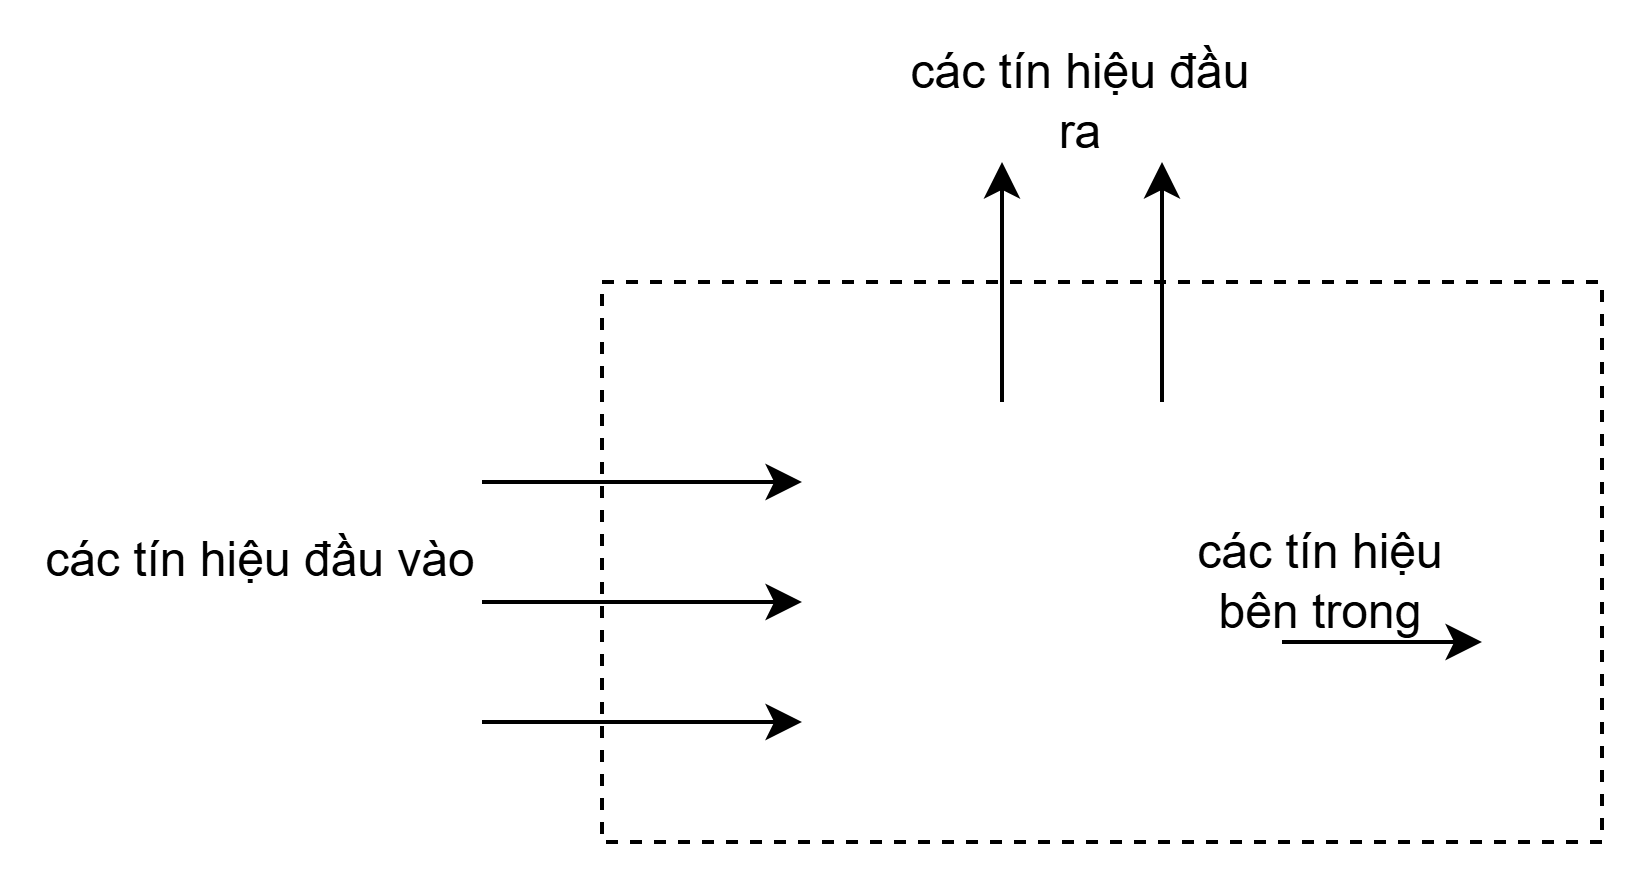
\includegraphics[width=0.7\linewidth]{figures/boxSym.png}
	\caption{Định nghĩa các tín hiệu ra vào một mô-đun}
	\label{fig:boxSym}
\end{figure}
\section{mô-đun MedianProcessing}
\subsection{mô-đun LineBuffer}
Nguyên lý hoạt động của mô-đun LineBuffer là khi có dữ liệu đầu vào, dữ liệu sẽ được ghi vào một vùng nhớ cụ thể, sau khi đạt đến một thời gian hoặc điều kiện đặt ra, dữ liệu từ vùng nhớ đã được ghi sẽ được đọc ra và thứ tự đầu ra sẽ theo nguyên lý FIFO (First In First Out, dữ liệu ghi trước sẽ được đọc ra trước). Hình \ref{fig:lineBuffArchitecture} mô tả kiến trúc RTL của mô-đun LineBuffer và hình \ref{fig:lineBufferTrans} mô tả sơ đồ chuyển trạng thái của bộ \textit{controller} cho mô-đun này. Có thể mô tả ngắn gọn cách thức hoạt động của mô-đun theo mô tả sau: Dữ liệu sẽ được đệm vào bộ nhớ, sau khi dữ liệu ở hàng đầu tiên được đệm (tức là lần đầu tiên bộ nhớ đầy) thì lúc này sẽ có tín hiệu cho phép dữ liệu ra, và quá trình này sẽ kết thúc khi toàn bộ dữ liệu đầu vào được đệm đến đầu ra. 


\textit{Số lượng chu kỳ từ lúc có dữ liệu vào đến khi có dữ liệu đầu ra: } \textbf{DEPTH}


\textit{Số lượng chu kỳ từ lúc có dữ liệu vào đến khi có dữ liệu đầu ra của mô-đun Buffer6Rows: } \textbf{3 * DEPTH}


\begin{figure}[!ht]
    \centering
    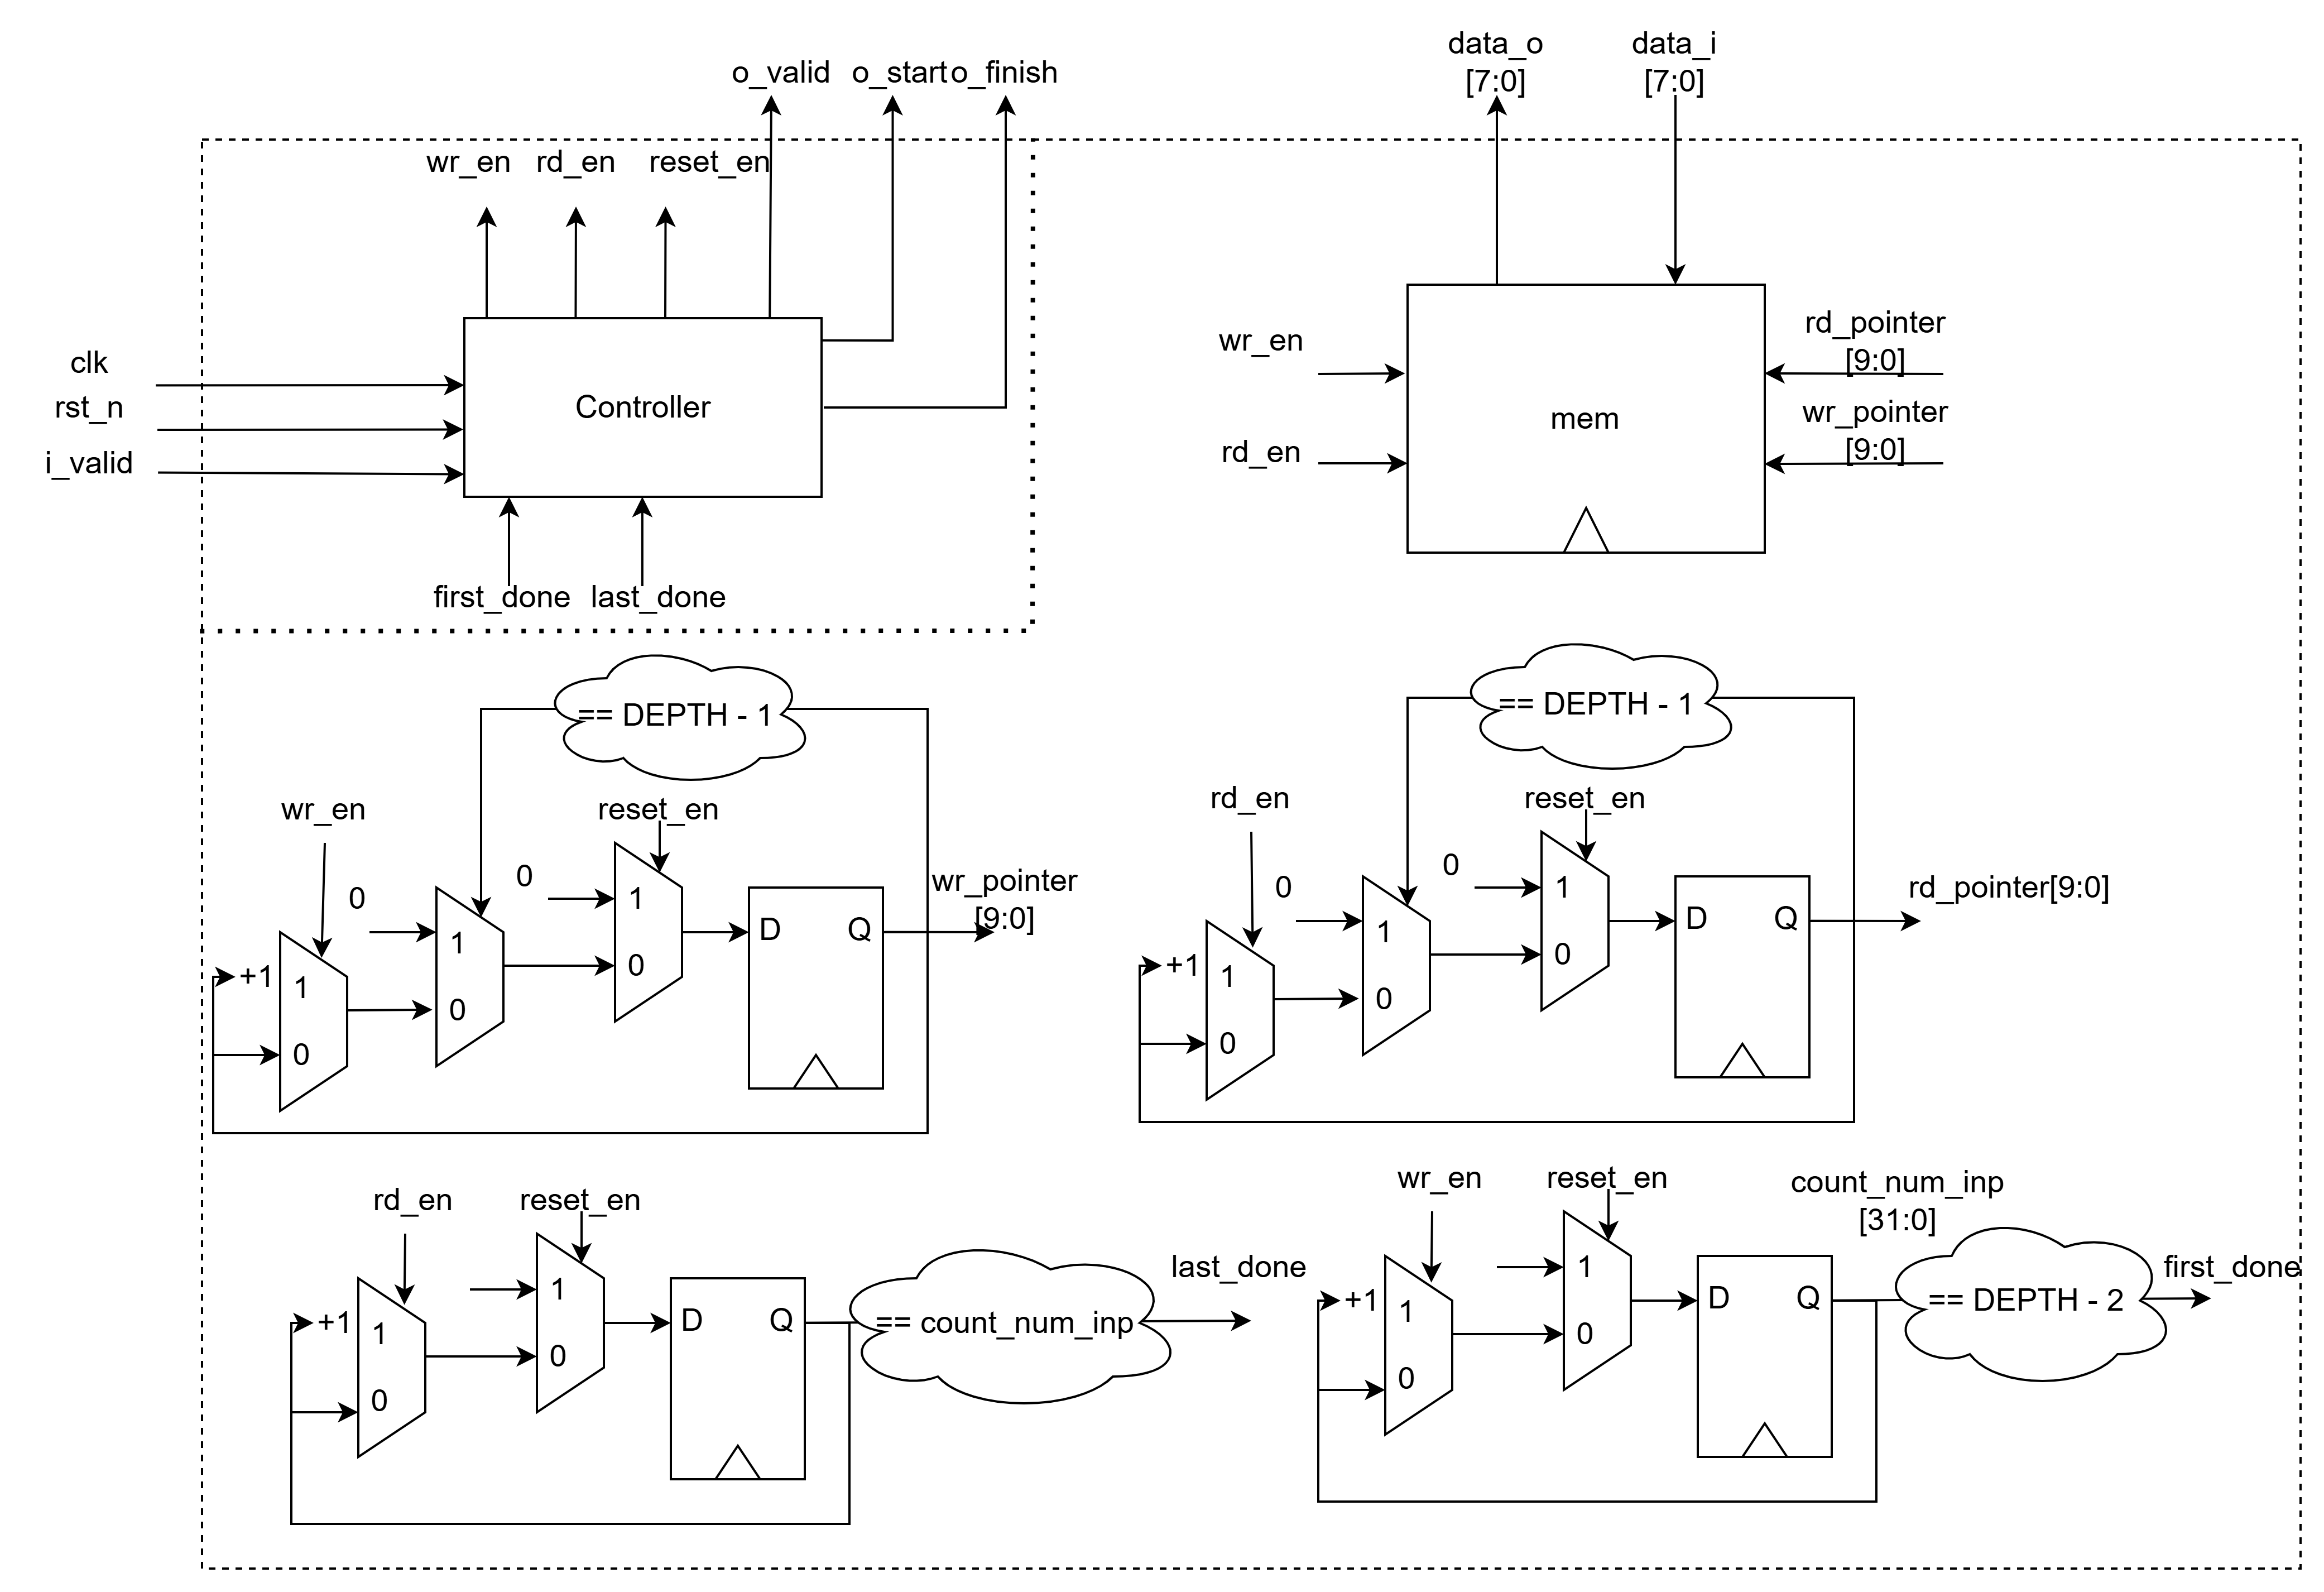
\includegraphics[width=\linewidth]{figures/lineBuffArchitecture.png}
    \caption{Mô tả RTL của mô-đun LineBuffer}
    \label{fig:lineBuffArchitecture}
\end{figure}


\begin{figure}[!ht]
    \centering
    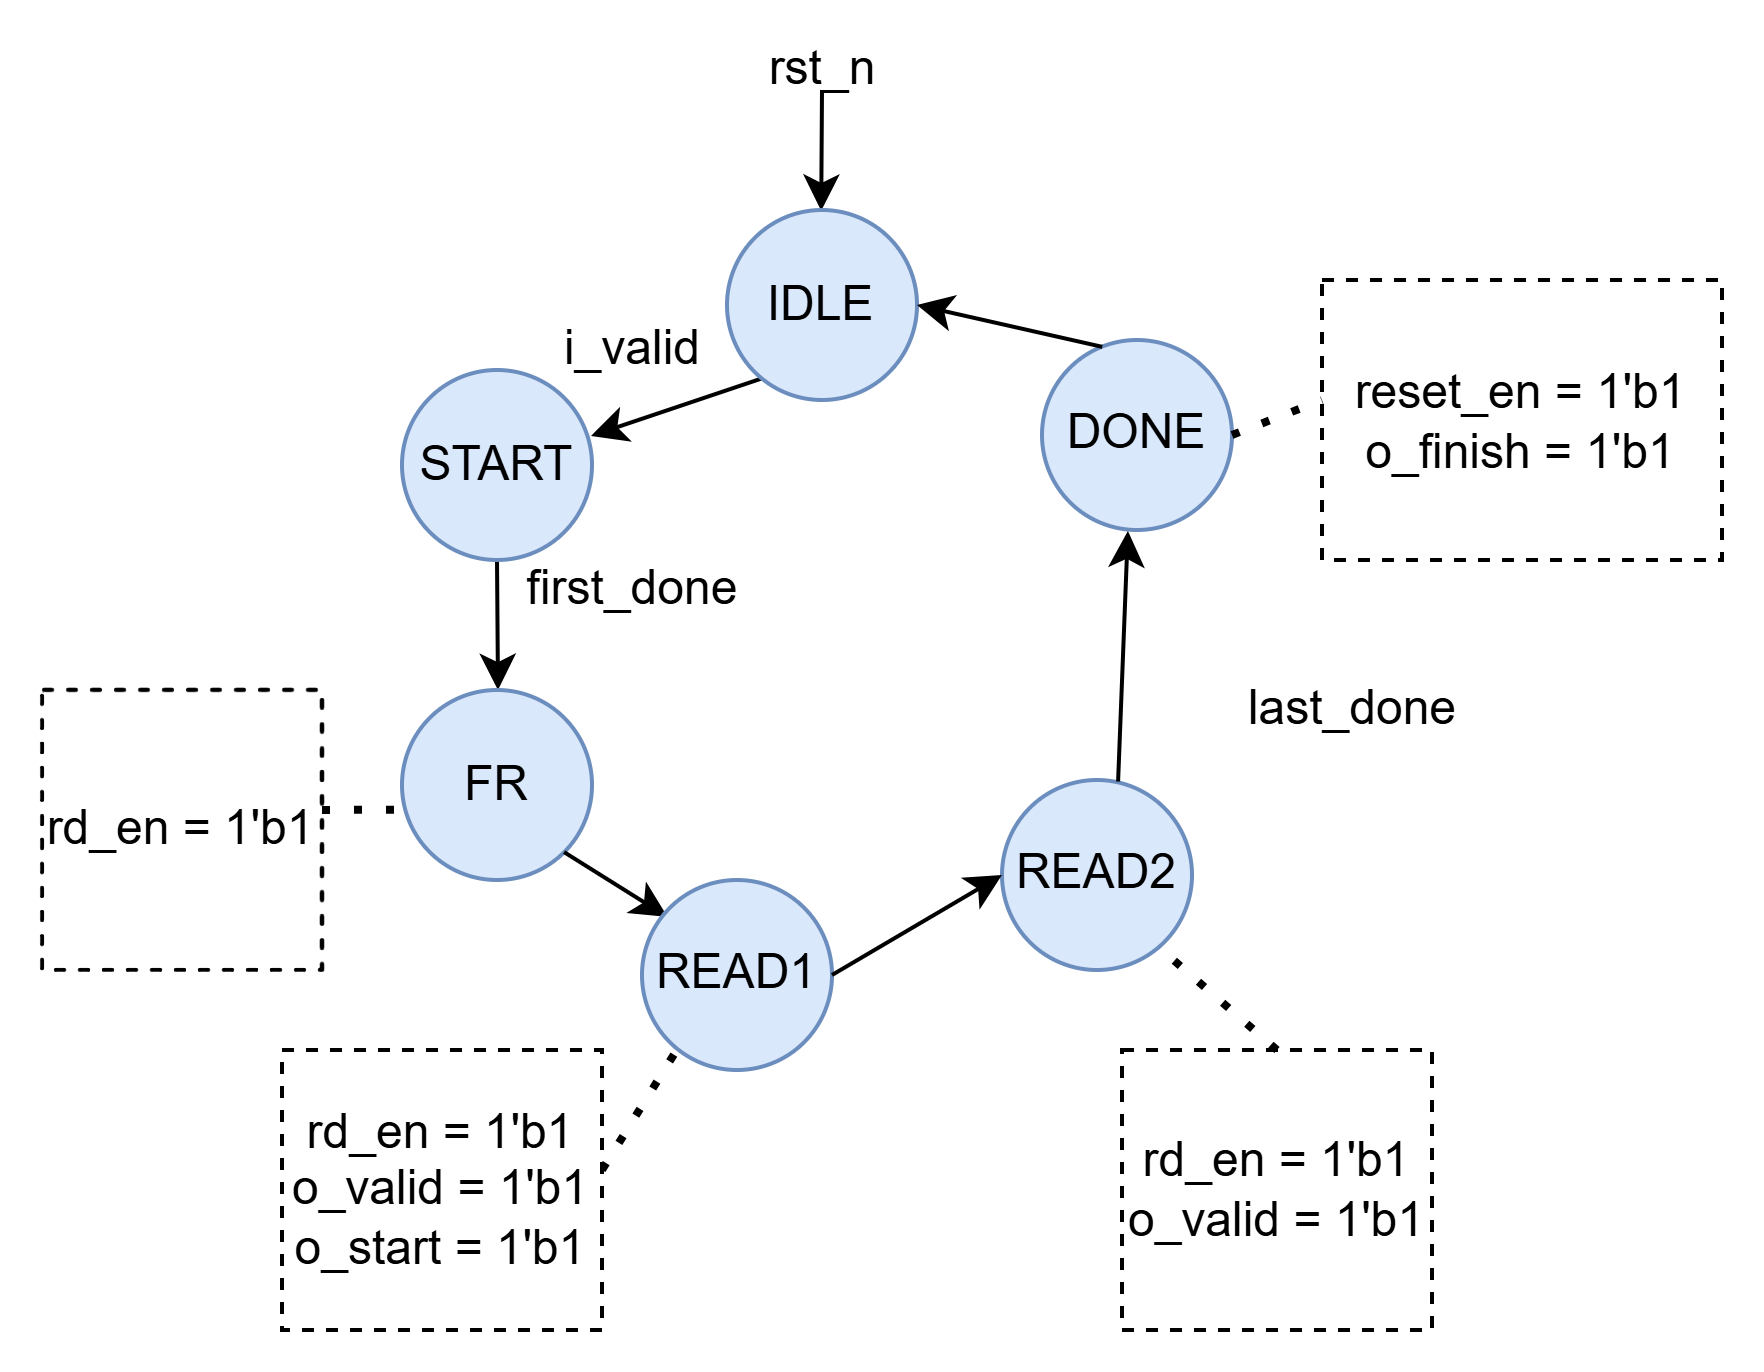
\includegraphics[width=0.8\linewidth]{figures/lineBufferTrans.png}
    \caption{Sơ đồ chuyển trạng thái của mô-đun LineBuffer}
    \label{fig:lineBufferTrans}
\end{figure}


\subsection{mô-đun ZeroPadding}
Mô-đun \textbf{ZeroPadding} sẽ được thiết kế riêng biệt cho ba loại cửa sổ là 3$\times$3, 5$\times$5 và 7$\times$7. Tuy nhiên, chúng đều sử dụng chung một bộ điều khiển, hoạt động theo mô tả ở hình~\ref{fig:zeroPaddingTrans}. Bộ điều khiển này bao gồm bốn trạng thái: \textbf{IDLE}, \textbf{START}, \textbf{DATA} và \textbf{DONE}.

Trạng thái \textbf{START} có chức năng chờ cho đến khi dữ liệu được đệm trong mô-đun ZeroPadding đủ để đáp ứng yêu cầu đầu ra của cửa sổ. Ví dụ, với cửa sổ 3$\times$3, khi xử lý ở rìa ảnh sẽ cần đệm thêm các giá trị 0. Khi đó, trong mô-đun cần có sẵn ít nhất hai điểm ảnh, để sau khi đệm thêm một điểm ảnh 0 sẽ đủ ba điểm ảnh cho một hàng hoặc một cột của cửa sổ.

Trạng thái \textbf{DATA} có chức năng cho phép xuất dữ liệu đầu ra. Khi tín hiệu \textbf{o\_en} ở mức logic 1, các thanh ghi chốt (flip-flop) chứa dữ liệu đầu ra mới được phép truyền dữ liệu ra ngoài. Ví dụ, trong hình~\ref{fig:zero3x3Architecture2}, để dữ liệu đầu ra \textbf{d0\_o} được phép phát ra ngoài, điều kiện là \textit{o\_en} \,\&\, (\textit{i\_row\_lt\_1} \,|\, \textit{i\_col\_lt\_1}). Điều kiện này cũng được áp dụng tương tự cho tất cả các phiên bản khác của mô-đun ZeroPadding.

\begin{figure}[!ht]
    \centering
    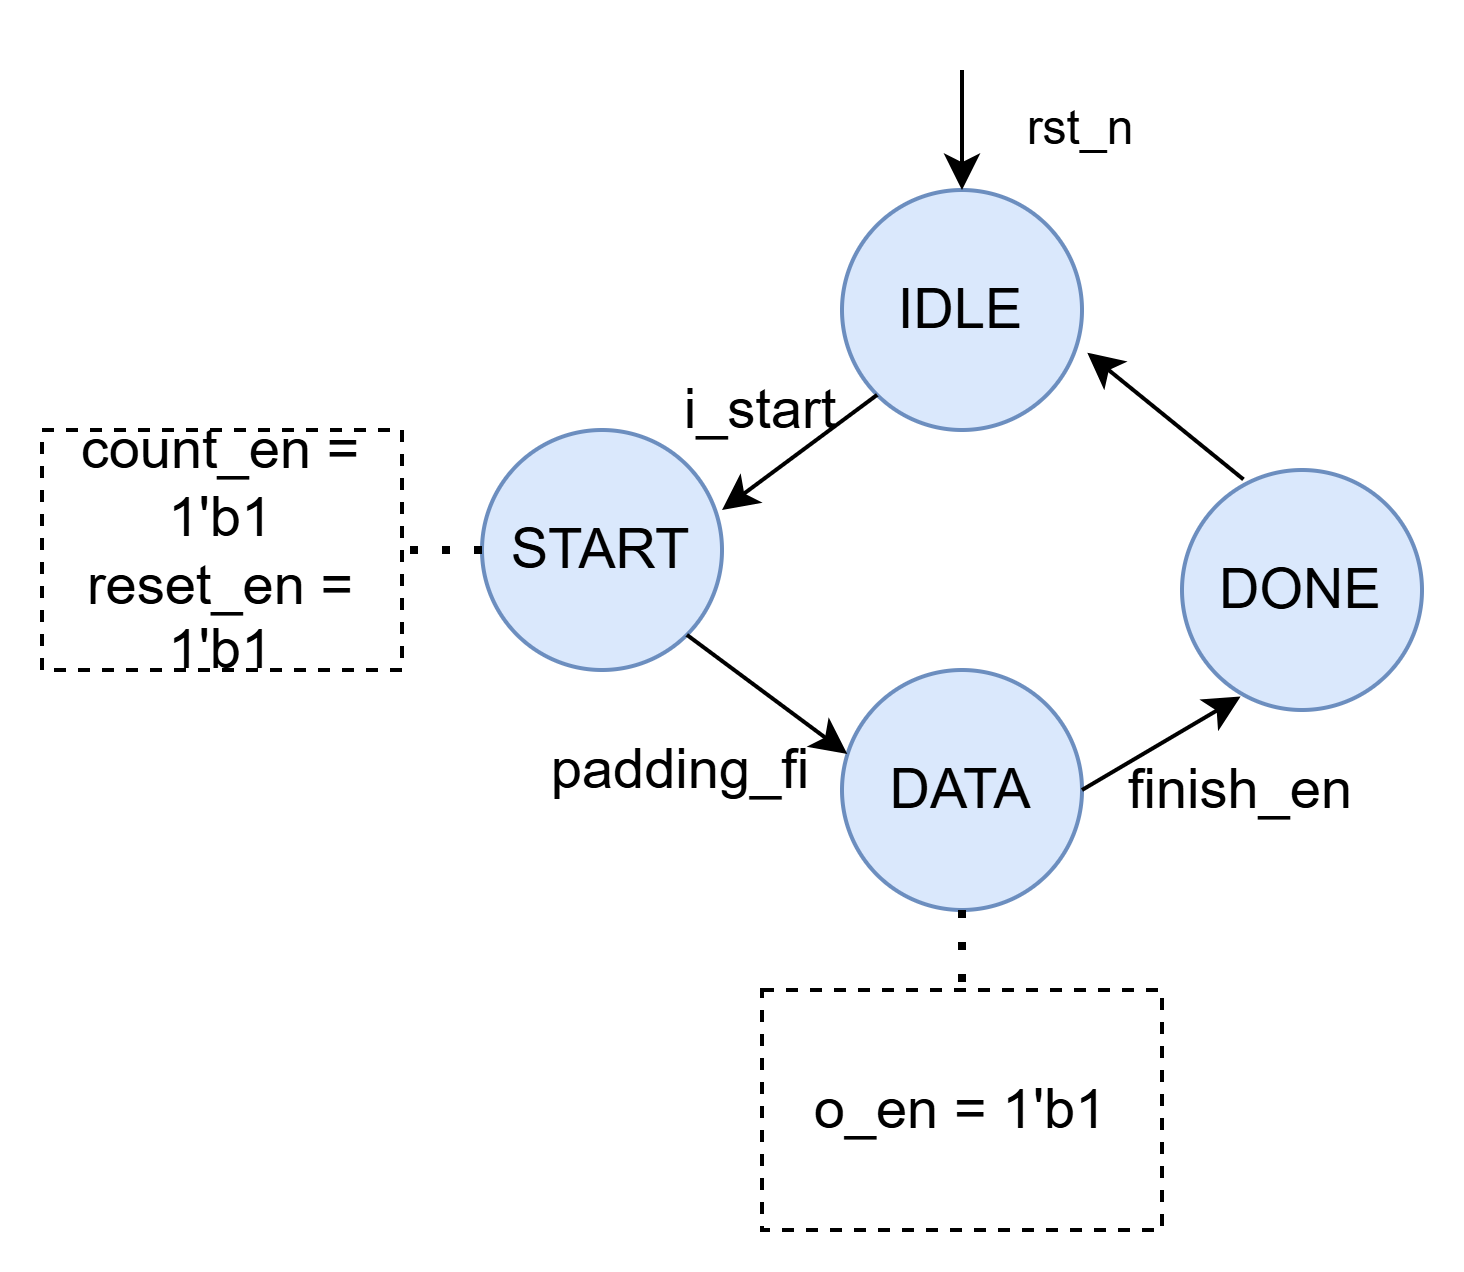
\includegraphics[width=0.6\linewidth]{figures/zeroPaddingTrans.png}
    \caption{Sơ đồ chuyển trạng thái của mô-đun ZeroPadding}
    \label{fig:zeroPaddingTrans}
\end{figure}


\subsubsection{Cửa sổ 3x3}
Hình \ref{fig:zero3x3Architecture1} mô tả kiến trúc RTL đối với bộ ZeroPadding của cửa sổ 3x3, dữ liệu đầu vào của từng hàng sẽ được đệm qua 3 thanh ghi để tạo ra 3 giá trị ứng với mỗi hàng của cửa sổ đầu ra. Dữ liệu đầu ra sẽ dựa vào các điều kiện như ở hình \ref{fig:zero3x3Architecture2}, chính là các tín hiệu điều khiển bộ mạch ghép kênh (mux) để lựa chọn đầu ra là dữ liệu nào.
\begin{figure}[!ht]
    \centering
    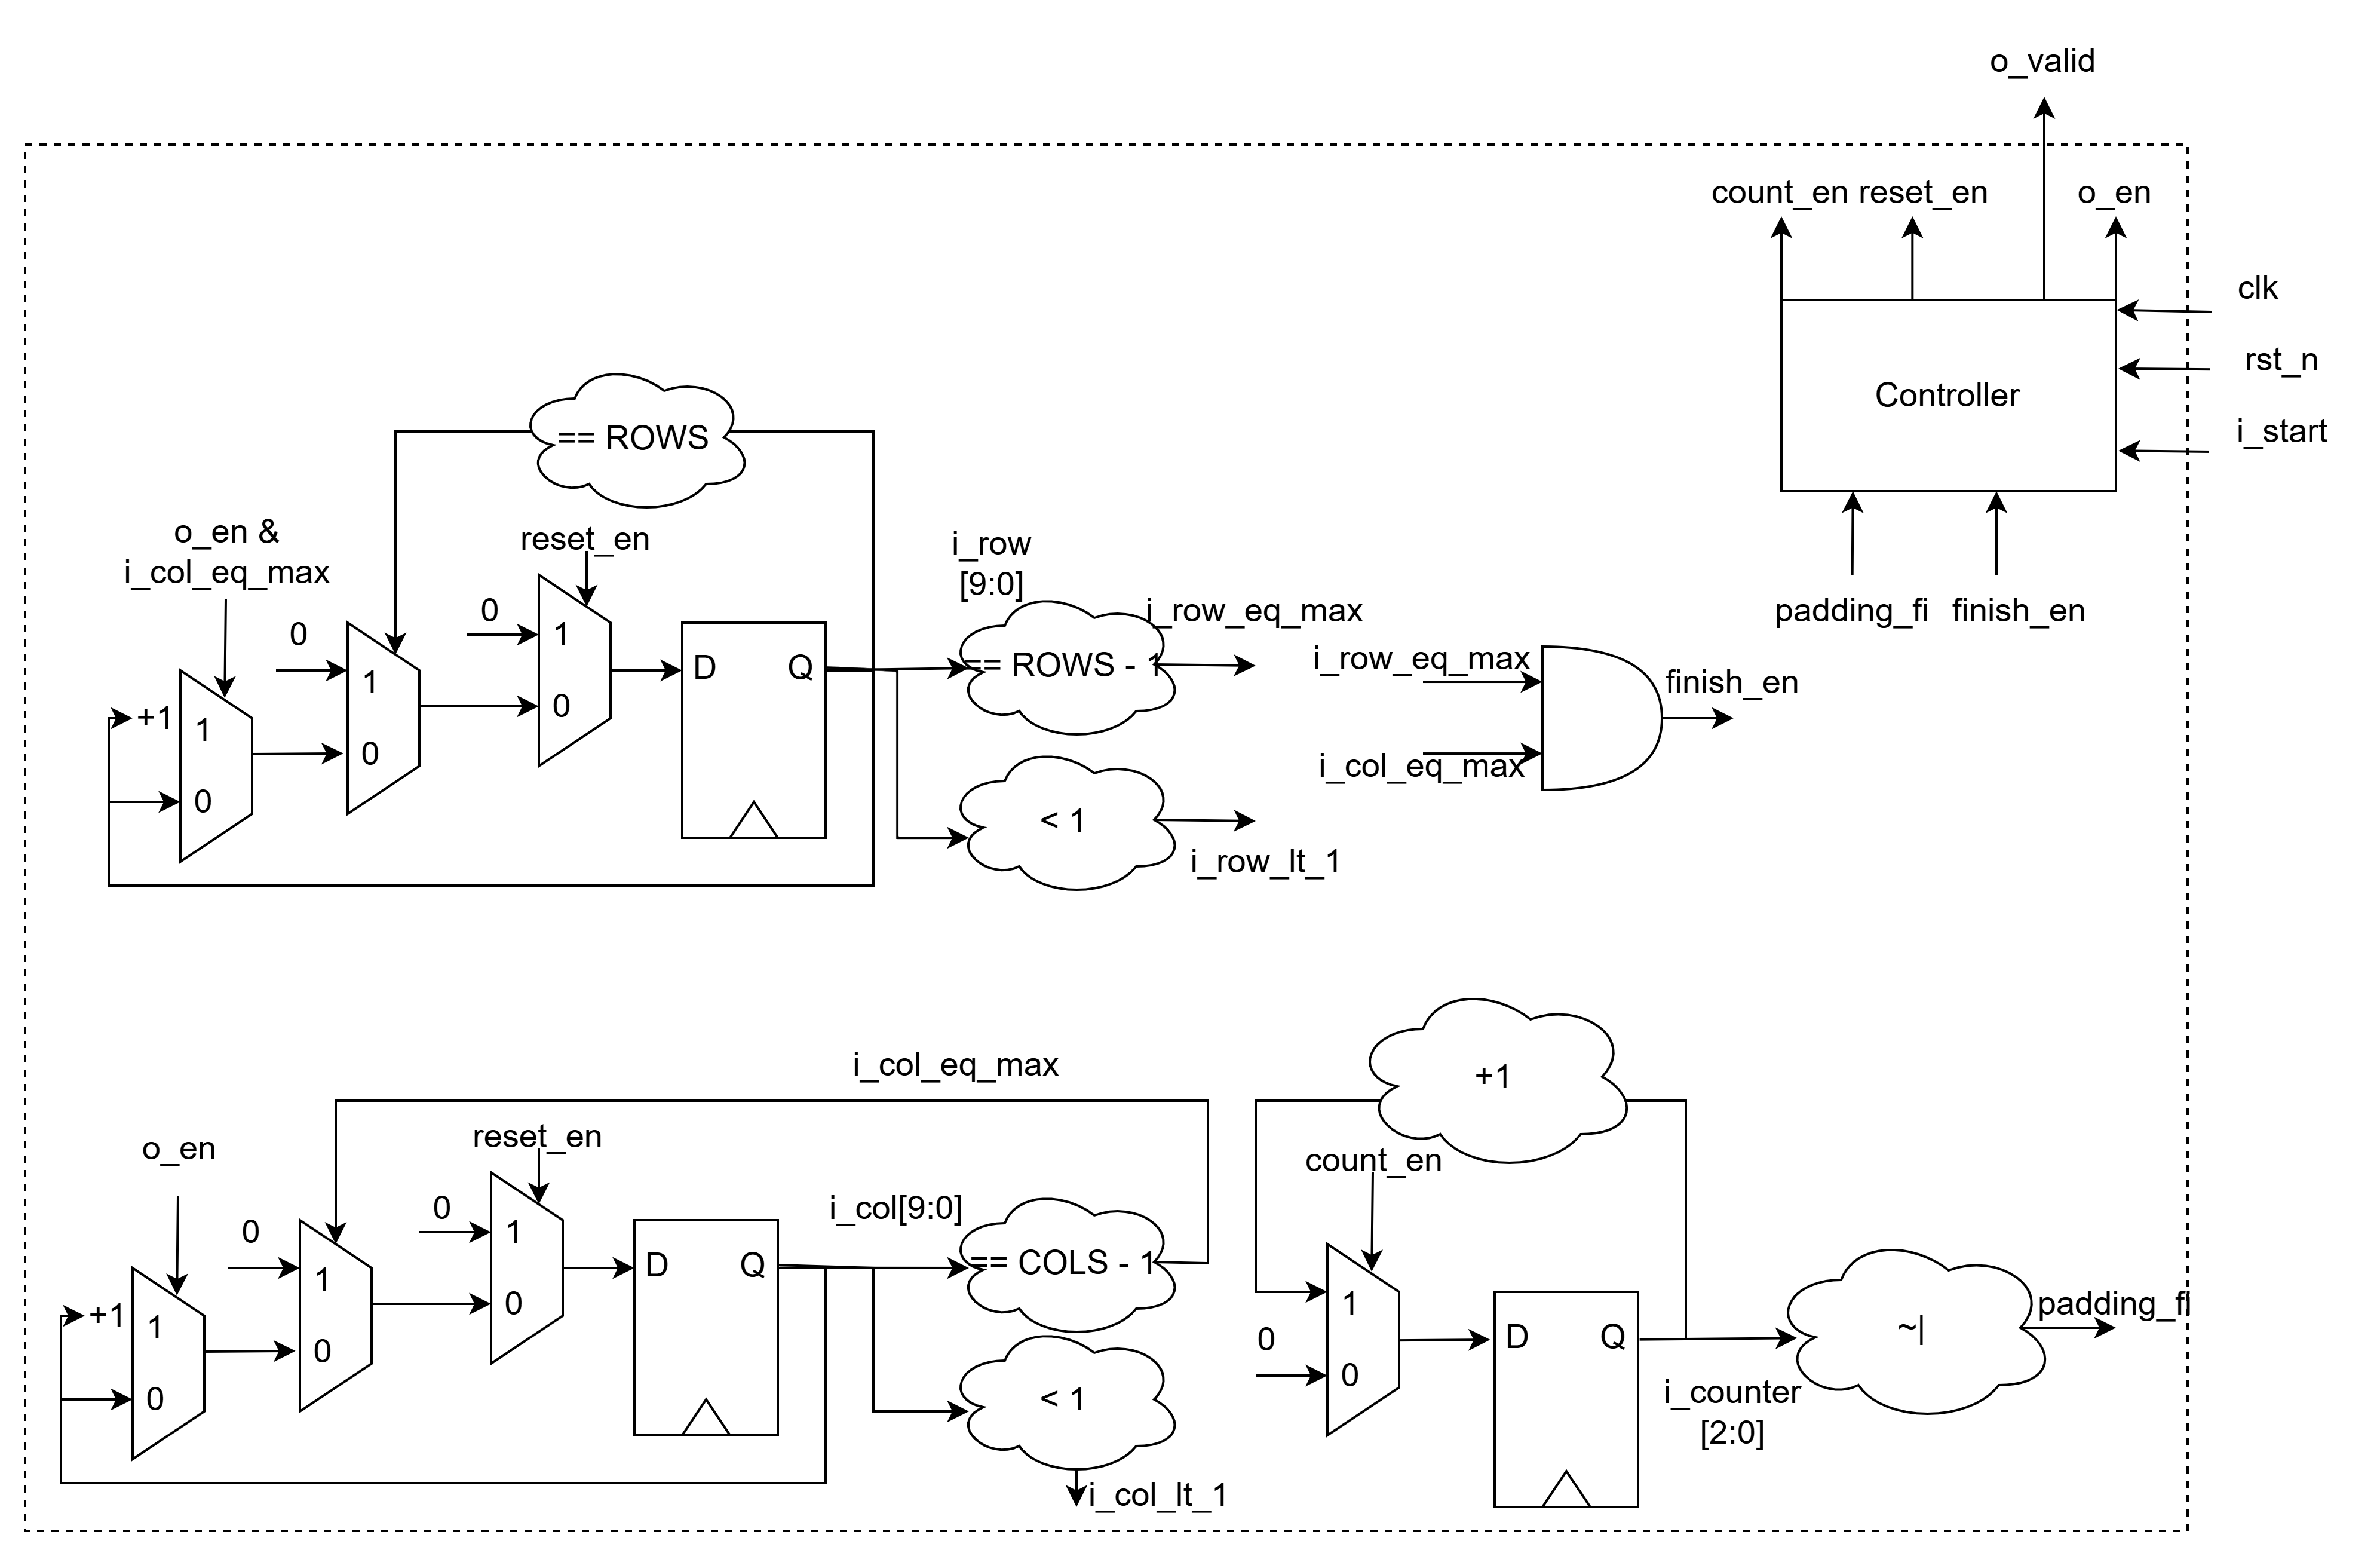
\includegraphics[width=\linewidth]{figures/zero3x3Architecture1.png}
    \caption{Mô tả RTL (1) của mô-đun ZeroPadding ứng với cửa sổ 3x3}
    \label{fig:zero3x3Architecture1}
\end{figure}

\begin{figure}[!ht]
    \centering
    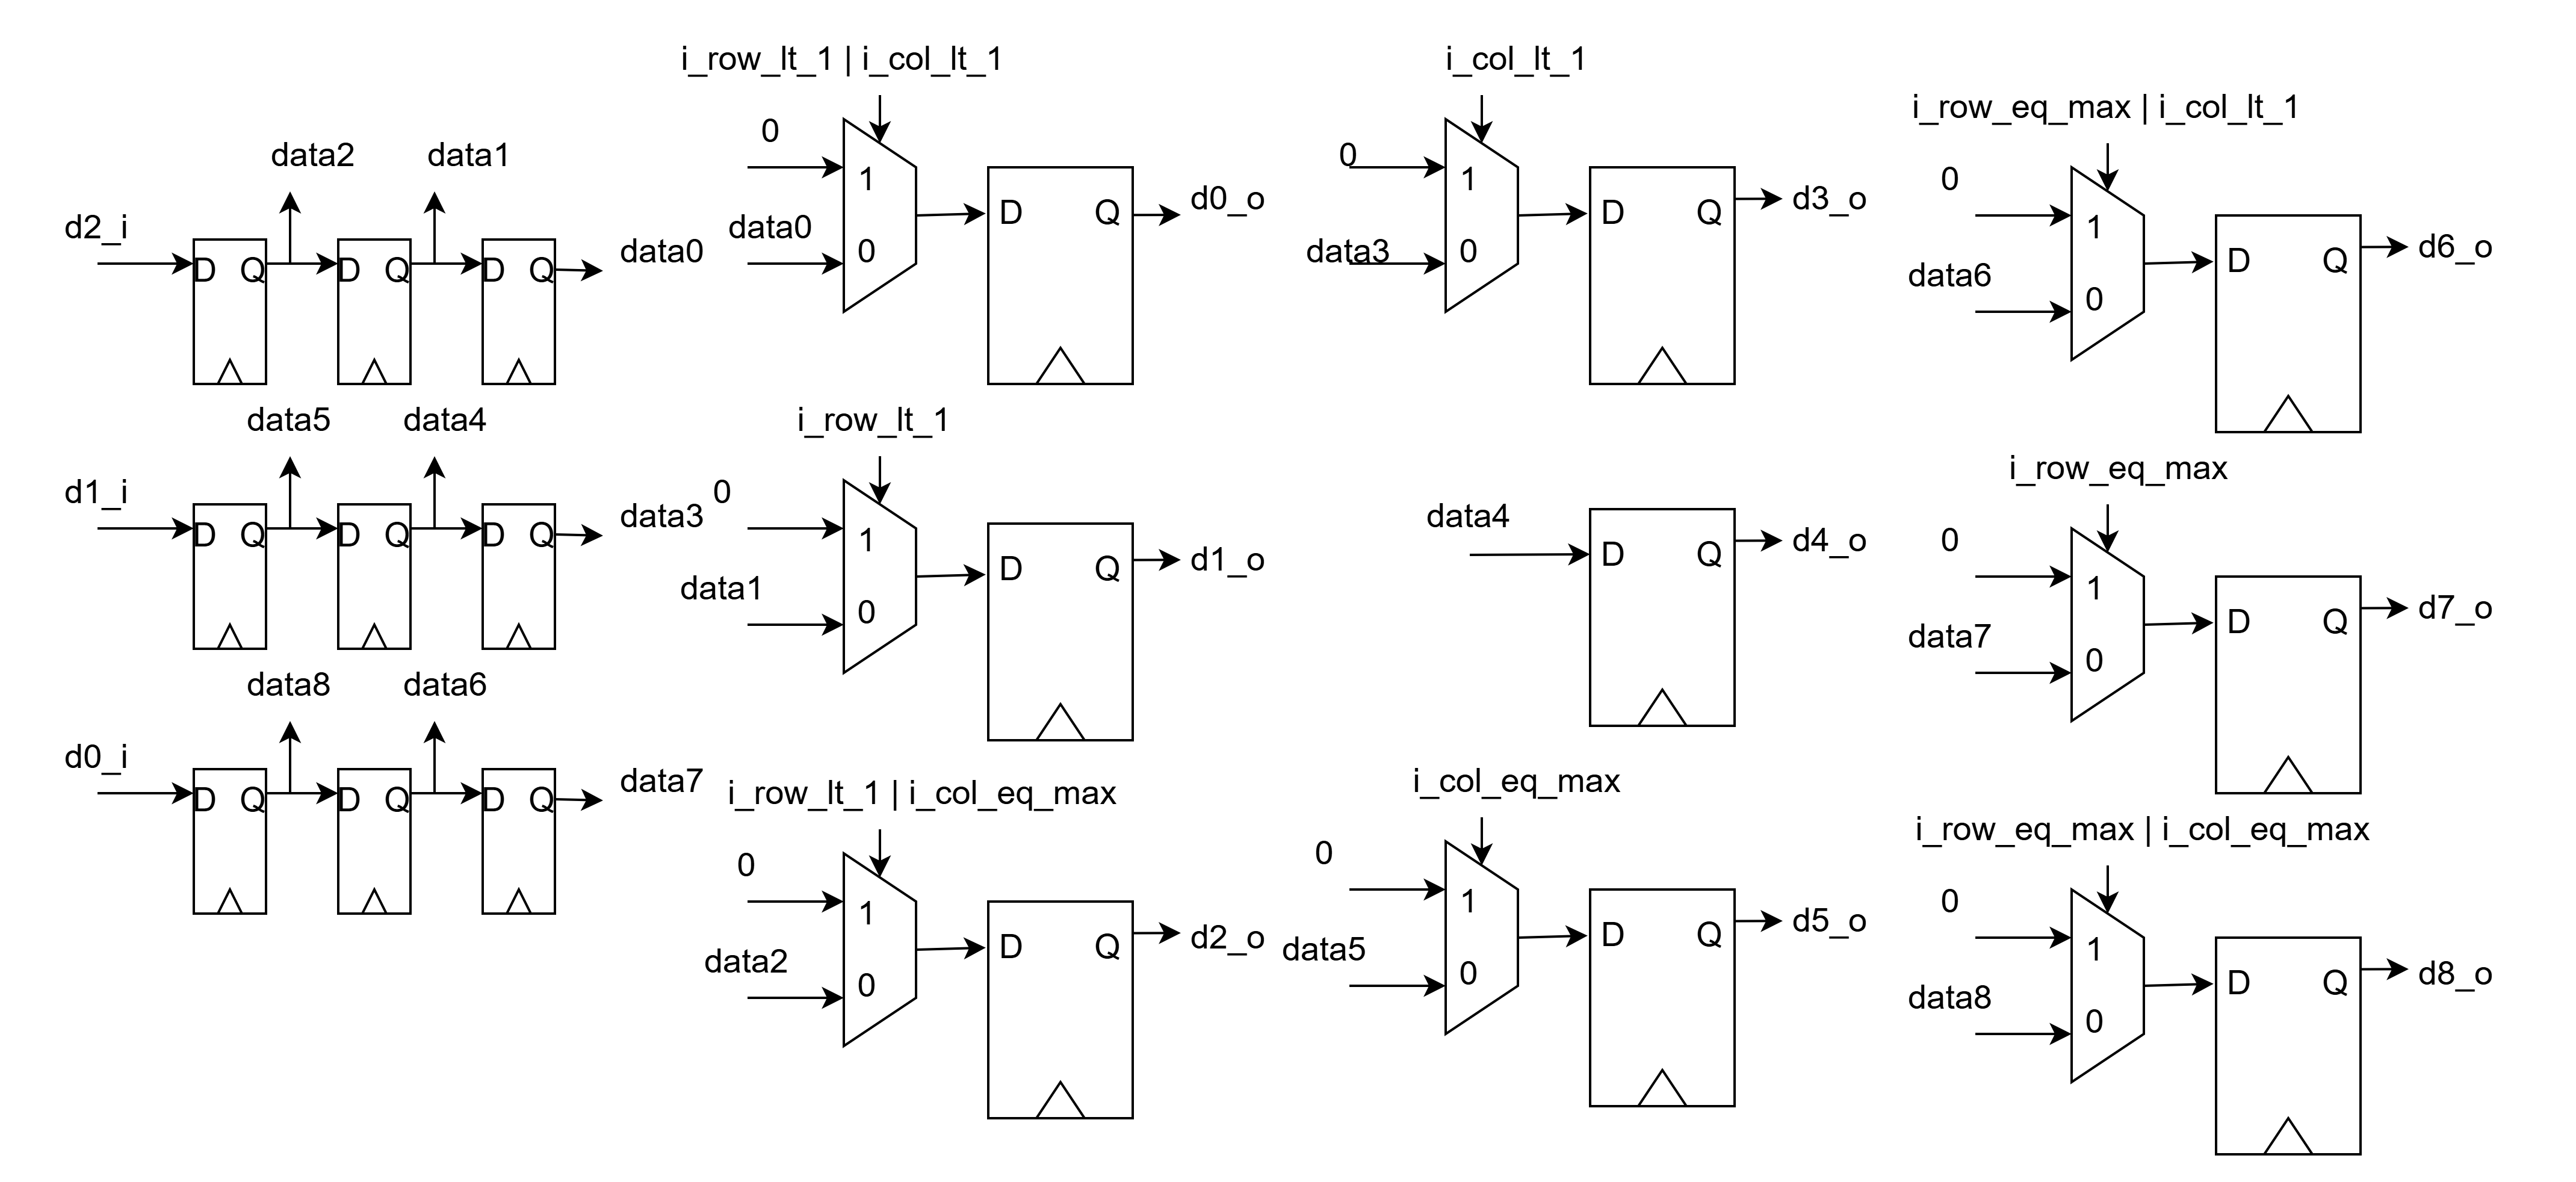
\includegraphics[width=\linewidth]{figures/zero3x3Architecture2.png}
    \caption{Mô tả RTL (2) của mô-đun ZeroPadding ứng với cửa sổ 3x3}
    \label{fig:zero3x3Architecture2}
\end{figure}


\textit{
Bởi vì đối với các cửa sổ 5x5 và 7x7, số lượng các đầu vào và điều kiện cho đầu ra là rất nhiều, khó có thể mô tả bằng hình vẽ, do đó sinh viên sẽ đưa ra bảng giá trị tham chiếu và điều kiện cho từng giá trị đầu ra. }

\subsubsection{Cửa sổ 5x5}
Hình \ref{fig:zero5x5Architecture1} mô tả kiến trúc ở mức RTL cho mô-đun ZeroPadding ứng với cửa sổ đầu vào 5x5. Về cơ bản, nguyên lý hoạt động của mô-đun này tương tự như đối với cửa sổ 3x3, nhưng có thêm một vài điều kiện thêm cho đầu ra như i\_row\_gt\_row\_3, ... Những điều kiện cho đầu ra đã được mô tả chi tiết trong bảng \ref{tab:conditionForOutputZero5x5}. Cột điều kiện tương ứng với tín hiệu chọn cho bộ mạch ghép kênh, khi điều kiện đúng thì đầu ra sẽ là 0, khi điều kiện sai, dữ liệu đầu ra sẽ ứng với giá trị của giá trị tham chiếu đến.
\begin{figure}[!ht]
    \centering
    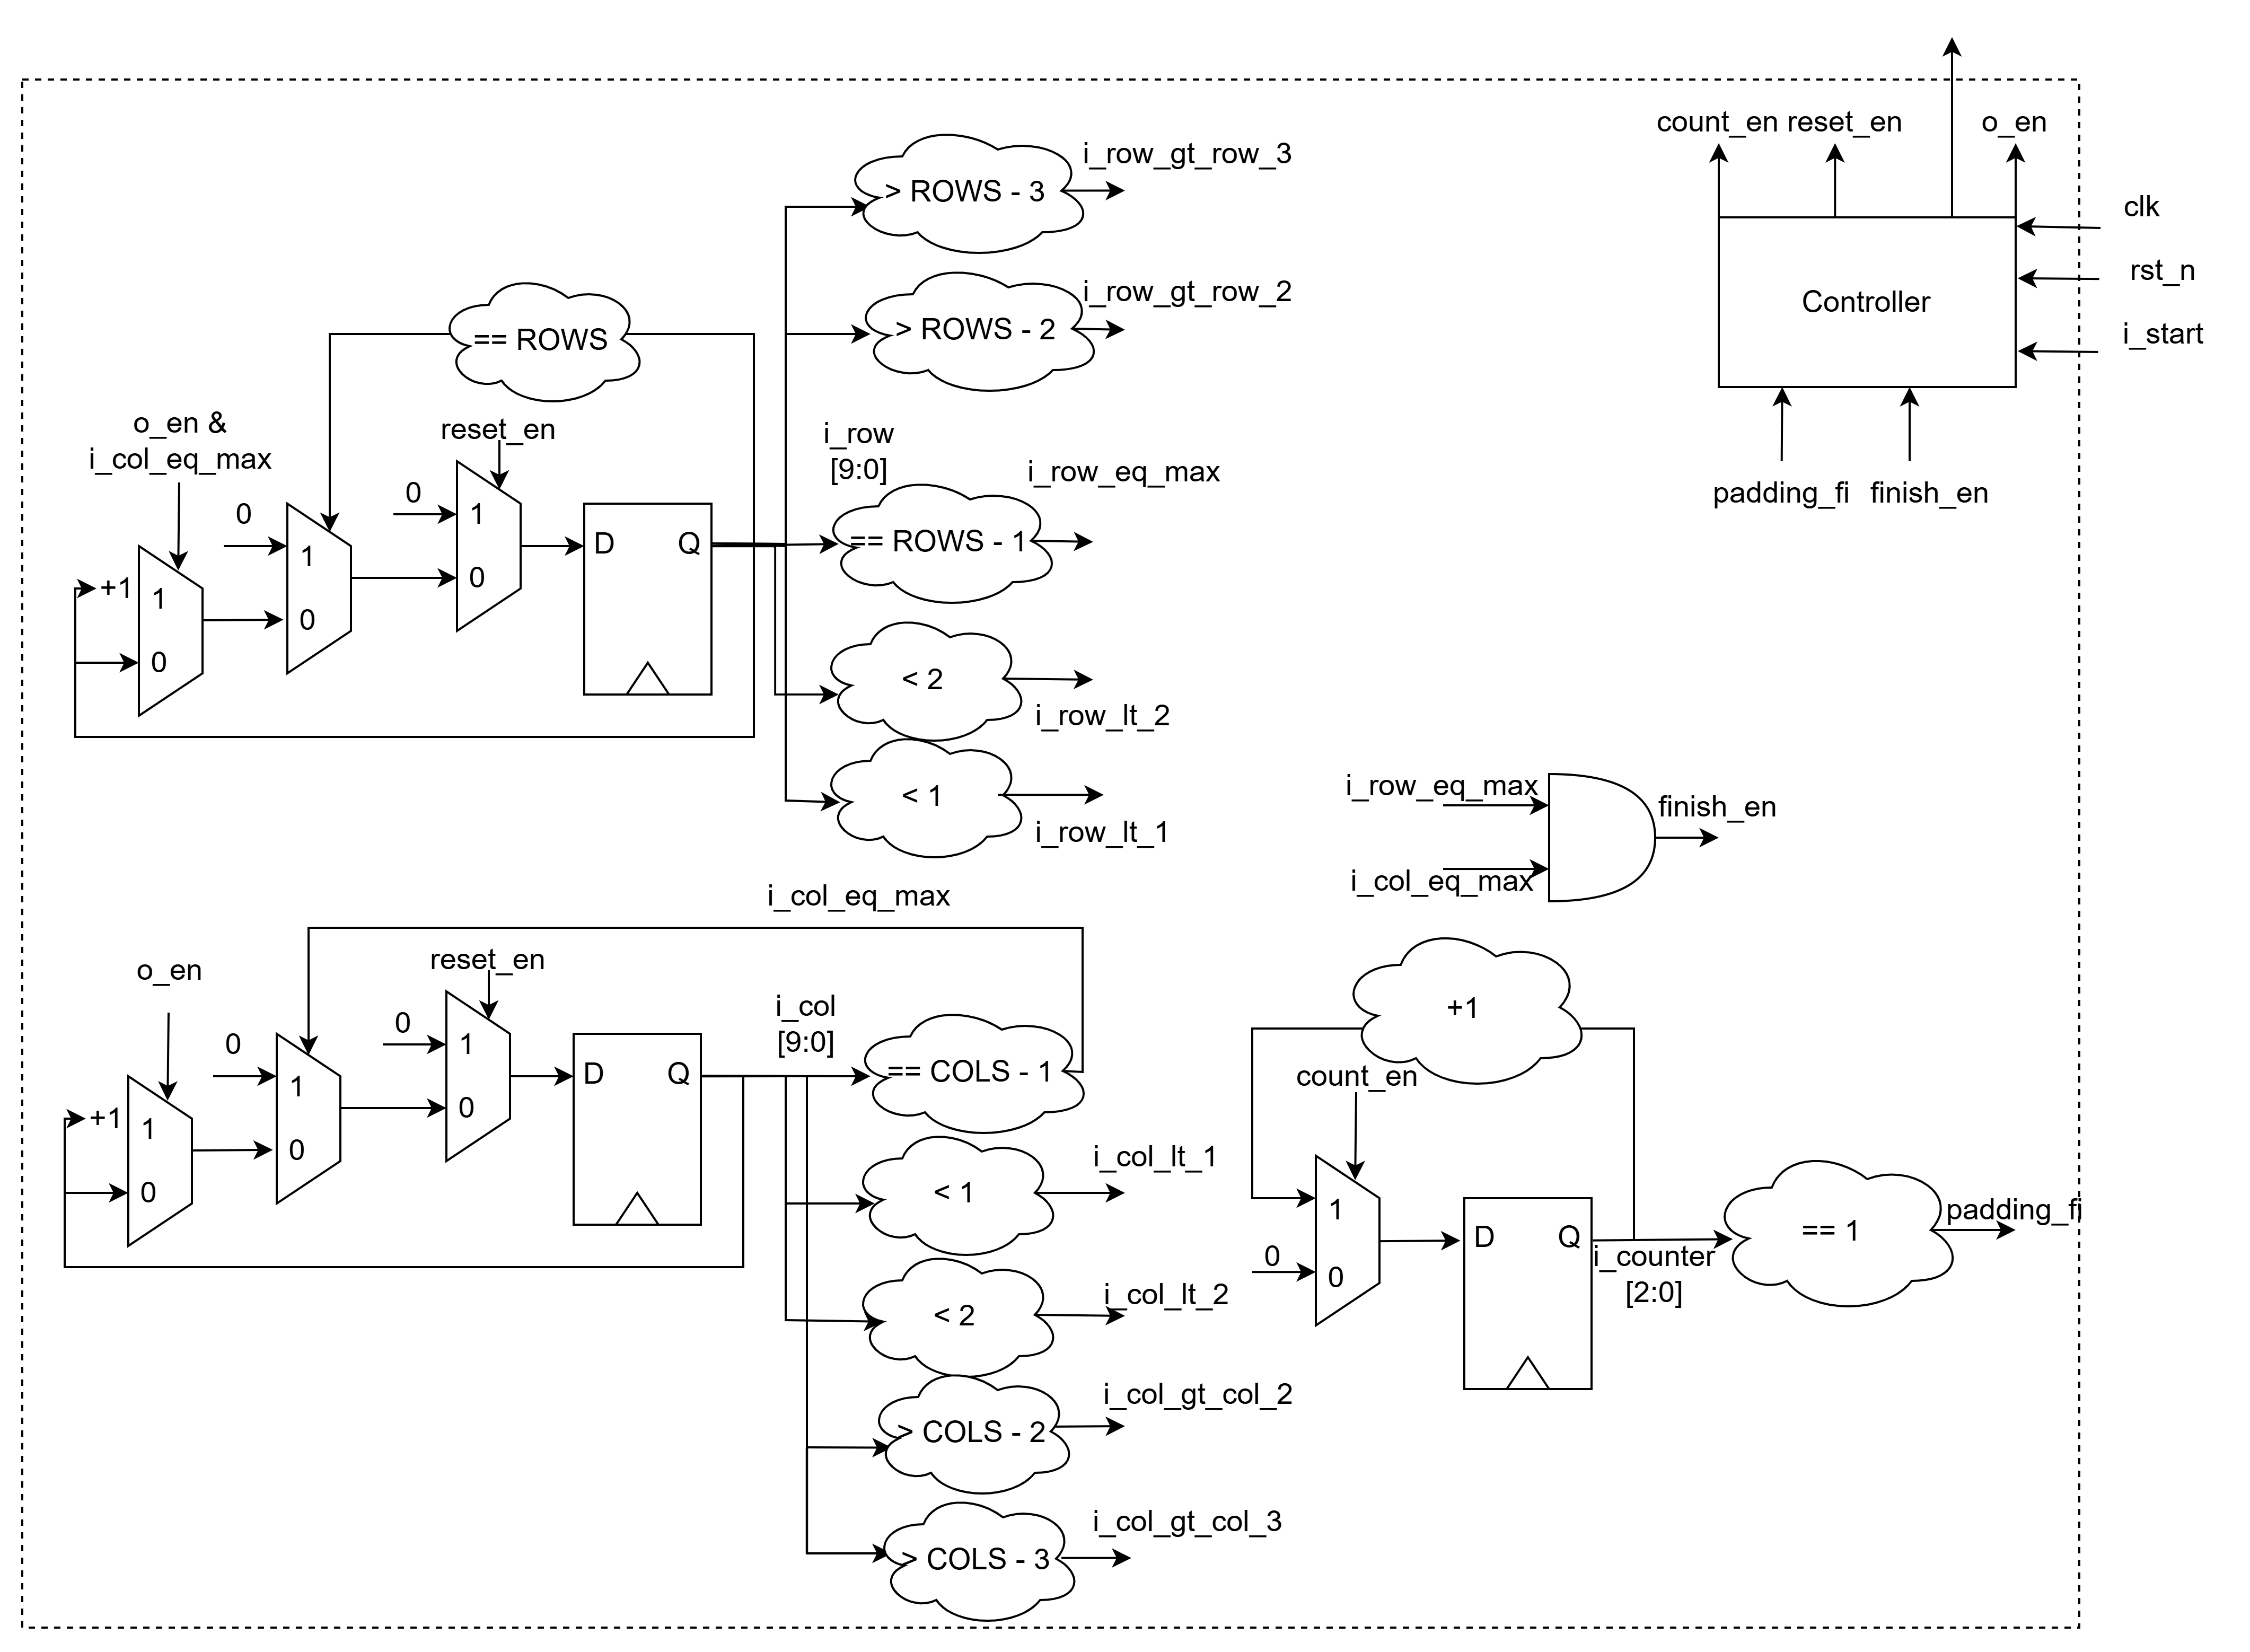
\includegraphics[width=0.9\linewidth]{figures/zero5x5Architecture1.png}
    \caption{Mô tả RTL của mô-đun ZeroPadding ứng với cửa sổ 5x5}
    \label{fig:zero5x5Architecture1}
\end{figure}


\begin{table}[!ht]
    \centering
    \renewcommand{\arraystretch}{1.4}
        \caption{Bảng điều kiện cho dữ liệu đầu ra ứng với cửa sổ 5x5}
    \begin{tabular}{|p{2.2cm} p{7cm} p{4cm}|}
        \hline
        \rowcolor{gray!30}
        \textbf{Tên đầu ra} & \textbf{Điều kiện} & \textbf{Giá trị tham chiếu} \\
        \hline
        d0\_o  & i\_row\_lt\_2 $\vert$ i\_col\_lt\_2         & data0  \\ \hline
        d1\_o  & i\_row\_lt\_2 $\vert$ i\_col\_lt\_1         & data1  \\ \hline
        d2\_o  & i\_row\_lt\_2                                & data2  \\ \hline
        d3\_o  & i\_row\_lt\_2 $\vert$ i\_col\_gt\_col\_2     & data3  \\ \hline
        d4\_o  & i\_row\_lt\_2 $\vert$ i\_col\_gt\_col\_3     & data4  \\ \hline
        d5\_o  & i\_row\_lt\_1 $\vert$ i\_col\_lt\_2         & data5  \\ \hline
        d6\_o  & i\_row\_lt\_1 $\vert$ i\_col\_lt\_1         & data6  \\ \hline
        d7\_o  & i\_row\_lt\_1                                & data7  \\ \hline
        d8\_o  & i\_row\_lt\_1 $\vert$ i\_col\_gt\_col\_2     & data8  \\ \hline
        d9\_o  & i\_row\_lt\_1 $\vert$ i\_col\_gt\_col\_3     & data9  \\ \hline
        d10\_o & i\_col\_lt\_2                                & data10 \\ \hline
        d11\_o & i\_col\_lt\_1                                & data11 \\ \hline
        d12\_o & -- (không có điều kiện)                     & data12 \\ \hline
        d13\_o & i\_col\_gt\_col\_2                           & data13 \\ \hline
        d14\_o & i\_col\_gt\_col\_2                           & data14 \\ \hline
      d15\_o & i\_row\_gt\_row\_2 $\vert$ i\_col\_lt\_2     & data15 \\ \hline
      d16\_o & i\_row\_gt\_row\_2 $\vert$ i\_col\_lt\_1     & data16 \\ \hline
      d17\_o & i\_row\_gt\_row\_2                           & data17 \\ \hline
      d18\_o & i\_row\_gt\_row\_2 $\vert$ i\_col\_gt\_col\_2 & data18 \\ \hline
      d19\_o & i\_row\_gt\_row\_2 $\vert$ i\_col\_gt\_col\_3 & data19 \\ \hline
      d20\_o & i\_row\_gt\_row\_3 $\vert$ i\_col\_lt\_2     & data20 \\ \hline
      d21\_o & i\_row\_gt\_row\_3 $\vert$ i\_col\_lt\_1     & data21 \\ \hline
      d22\_o & i\_row\_gt\_row\_3                           & data22 \\ \hline
      d23\_o & i\_row\_gt\_row\_3 $\vert$ i\_col\_gt\_col\_2 & data23 \\ \hline
      d24\_o & i\_row\_gt\_row\_3 $\vert$ i\_col\_gt\_col\_3 & data24 \\ \hline
    \end{tabular}

    \label{tab:conditionForOutputZero5x5}
\end{table}

\newpage
\subsubsection{Cửa sổ 7x7}
Bảng \ref{tab:numberOfCycleZeroPadding} mô tả số chu kỳ cần thiết từ lúc có dữ liệu vào đến khi có dữ liệu ra của từng mô-đun ZeroPadding ứng với từng loại cửa sổ. Thời gian tính toán tính từ thời điểm mà tín hiệu i\_start chuyển trạng thái đến khi mà tín hiệu đầu ra o\_valid chuyển trạng thái.
\begin{table}[H]
	\centering
	\renewcommand{\arraystretch}{1.3}
		\caption{Số chu kỳ thực hiện của các mô-đun ZeroPadding}
	\begin{tabular}{|p{5cm} p{5cm} |}
		\hline
		\rowcolor{gray!30}
		\textbf{Tên mô-đun} & \textbf{Số chu kỳ}  \\
		\hline
		ZeroPadding3x3  & 3 chu kỳ
		\\ \hline
		ZeroPadding5x5 & 4 chu kỳ
		\\ \hline
		ZeroPadding7x7 & 5 chu kỳ
		\\ \hline
	\end{tabular}

	\label{tab:numberOfCycleZeroPadding}
\end{table}


\begin{figure}[!ht]
    \centering
    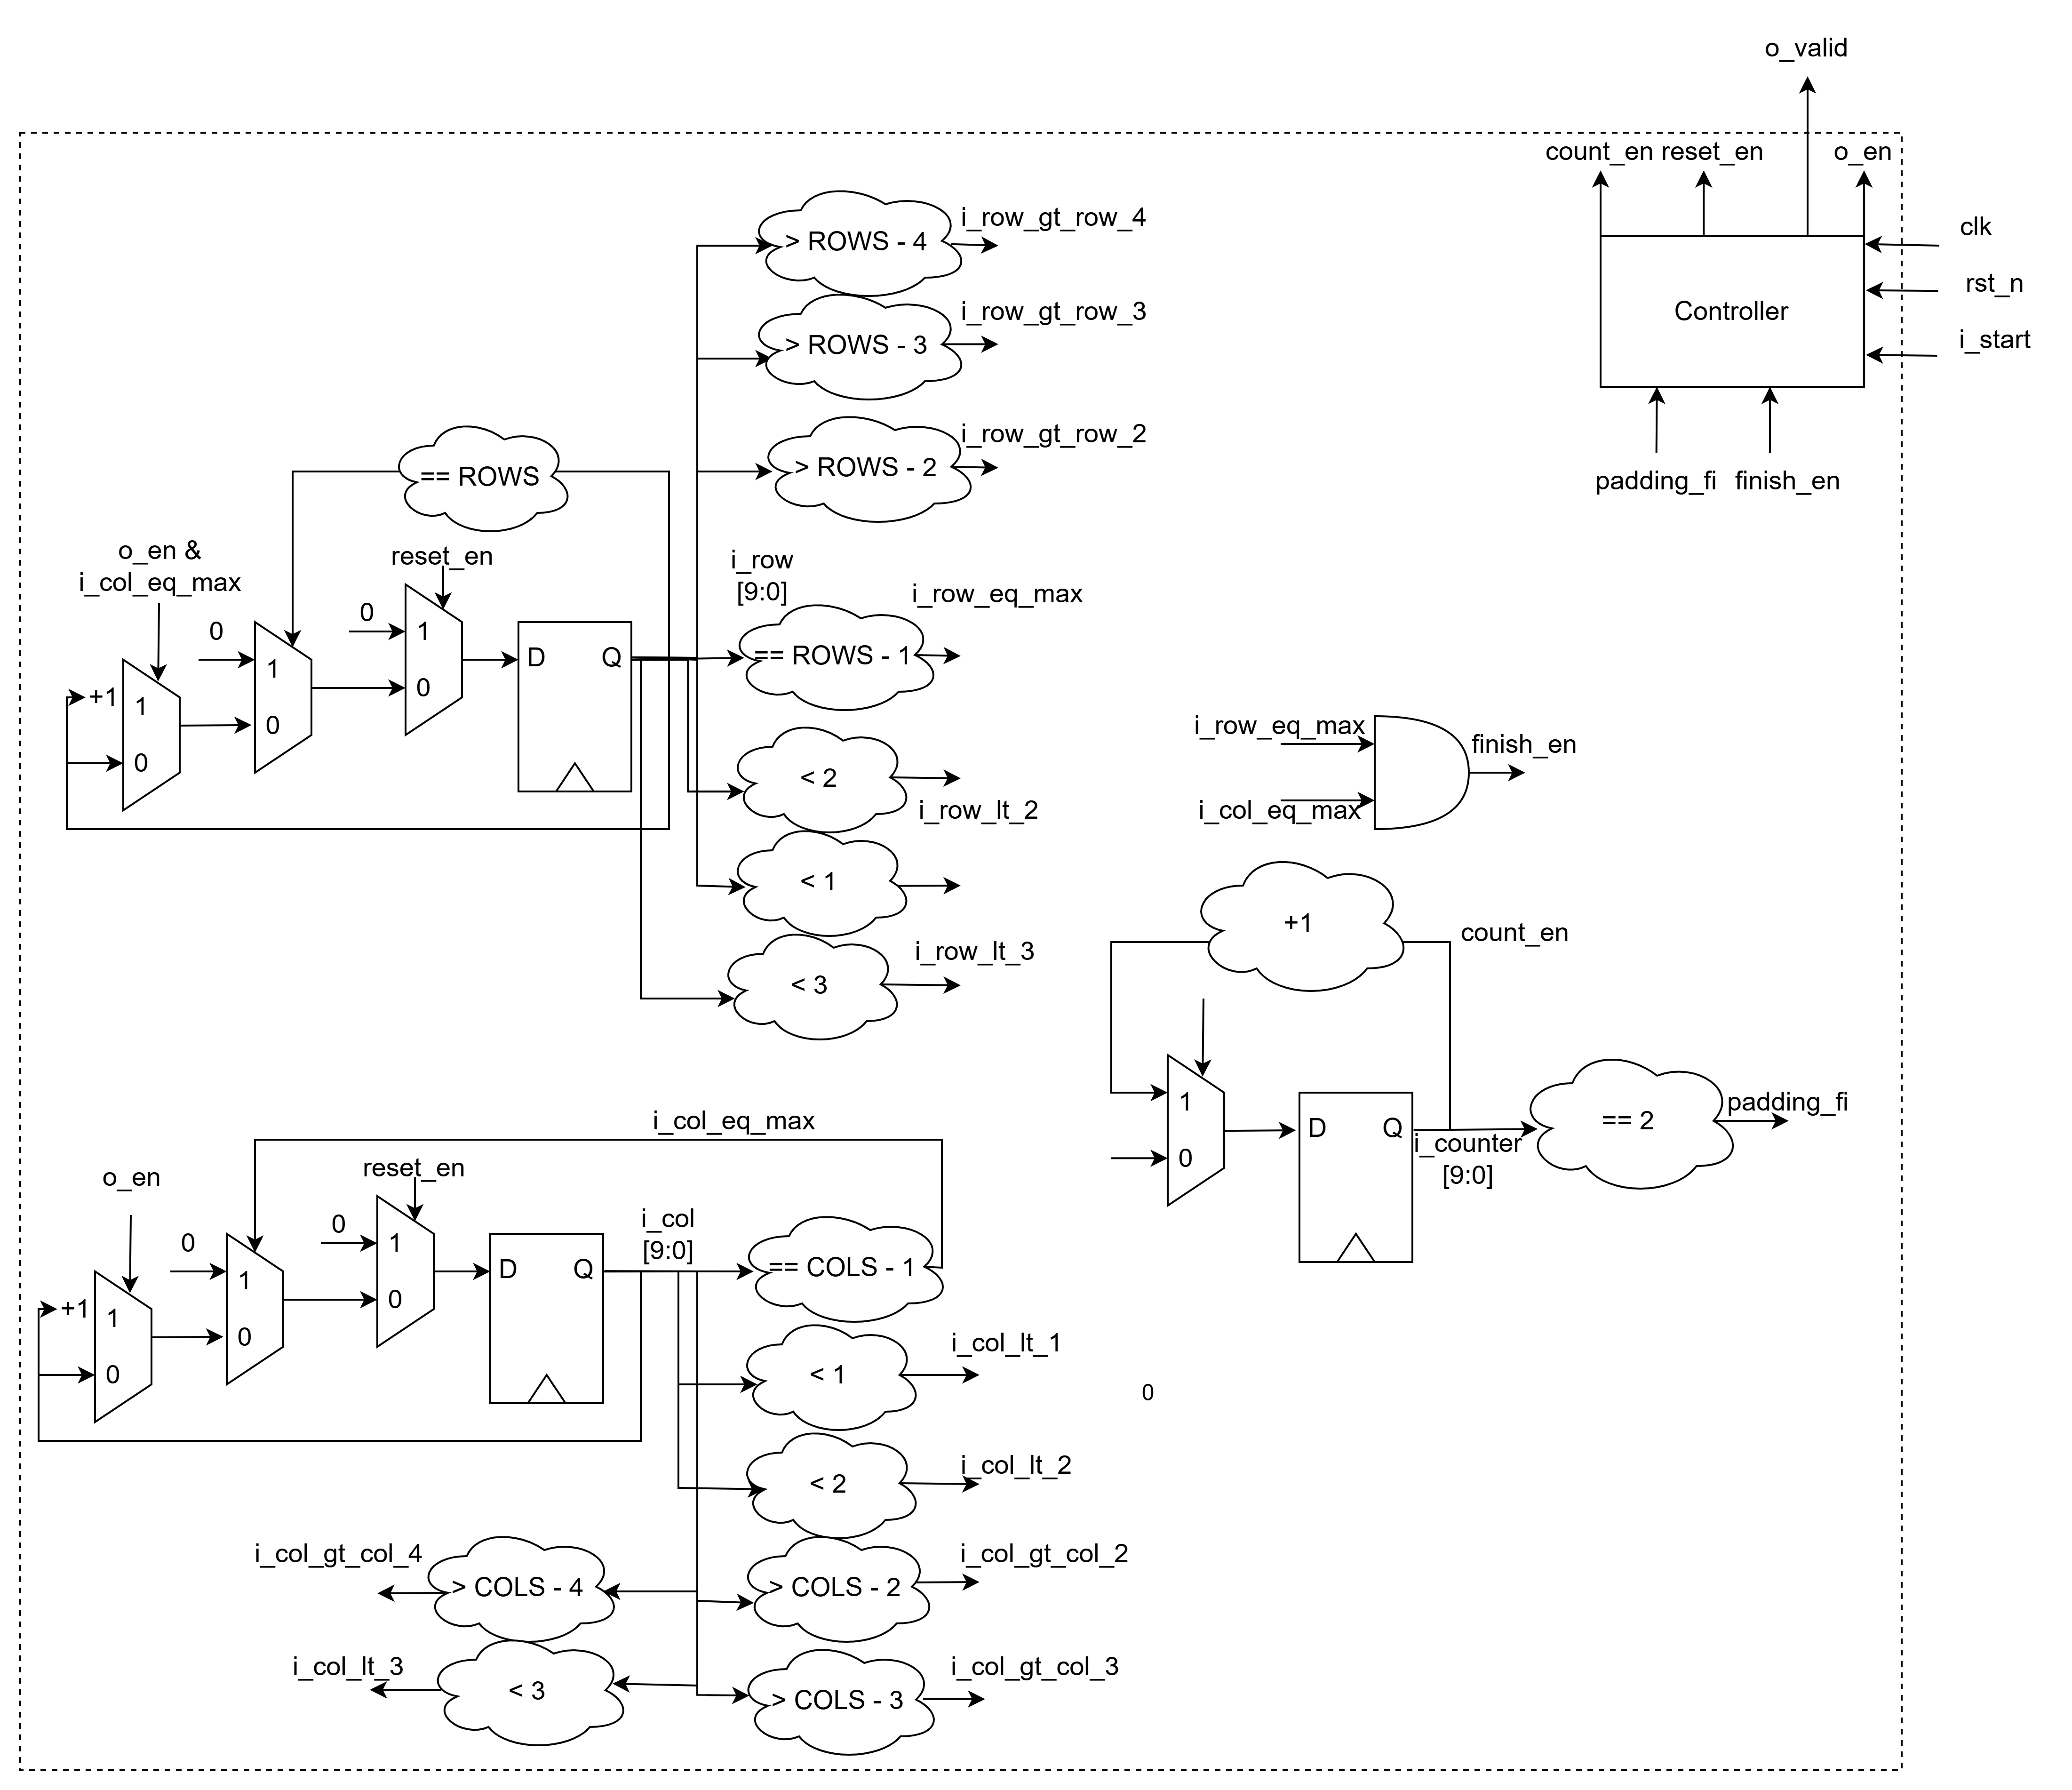
\includegraphics[width=\linewidth]{figures/zero7x7Architecture1.png}
    \caption{Mô tả RTL của mô-đun ZeroPadding ứng với cửa sổ 7x7}
    \label{fig:zero7x7Architecture1}
\end{figure}

\renewcommand{\arraystretch}{1}

\begin{longtable}{|p{3cm}|p{8cm}|p{4cm}|}
			\caption{Bảng điều kiện cho dữ liệu đầu ra ứng với cửa sổ 7x7} \\
	\hline
	\rowcolor{gray!30}
	\textbf{Tên đầu ra} & \textbf{Điều kiện} & \textbf{Giá trị tham chiếu} \\
	\hline
	\endfirsthead
	
	\hline
	\rowcolor{gray!30}
	\textbf{Tên đầu ra} & \textbf{Điều kiện} & \textbf{Giá trị tham chiếu} \\
	\hline
	\endhead
	d0\_o & i\_row\_lt\_3 $\vert$ i\_col\_lt\_3 & data0 \\
	d1\_o & i\_row\_lt\_3 $\vert$ i\_col\_lt\_2 & data1 \\
	d2\_o & i\_row\_lt\_3 $\vert$ i\_col\_lt\_1 & data2 \\
	d3\_o & i\_row\_lt\_3 & data3 \\
	d4\_o & i\_row\_lt\_3 $\vert$ i\_col\_gt\_col\_2 & data4 \\
	d5\_o & i\_row\_lt\_3 $\vert$ i\_col\_gt\_col\_3 & data5 \\
	d6\_o & i\_row\_lt\_3 $\vert$ i\_col\_gt\_col\_4 & data6 \\
	d7\_o & i\_row\_lt\_2 $\vert$ i\_col\_lt\_3 & data7 \\
	d8\_o & i\_row\_lt\_2 $\vert$ i\_col\_lt\_2 & data8 \\
	d9\_o & i\_row\_lt\_2 $\vert$ i\_col\_lt\_1 & data9 \\
	d10\_o & i\_row\_lt\_2 & data10 \\
	d11\_o & i\_row\_lt\_2 $\vert$ i\_col\_gt\_col\_2 & data11 \\
	d12\_o & i\_row\_lt\_2 $\vert$ i\_col\_gt\_col\_3 & data12 \\
	d13\_o & i\_row\_lt\_2 $\vert$ i\_col\_gt\_col\_4 & data13 \\
	d14\_o & i\_row\_lt\_1 $\vert$ i\_col\_lt\_3 & data14 \\
	d15\_o & i\_row\_lt\_1 $\vert$ i\_col\_lt\_2 & data15 \\
	d16\_o & i\_row\_lt\_1 $\vert$ i\_col\_lt\_1 & data16 \\
	d17\_o & i\_row\_lt\_1 & data17 \\
	d18\_o & i\_row\_lt\_1 $\vert$ i\_col\_gt\_col\_2 & data18 \\
	d19\_o & i\_row\_lt\_1 $\vert$ i\_col\_gt\_col\_3 & data19 \\
	d20\_o & i\_row\_lt\_1 $\vert$ i\_col\_gt\_col\_4 & data20 \\
	d21\_o & i\_col\_lt\_3 & data21 \\
	d22\_o & i\_col\_lt\_2 & data22 \\
	d23\_o & i\_col\_lt\_1 & data23 \\
	d24\_o & -- (không có điều kiện) & data24 \\
	d25\_o & i\_col\_gt\_col\_2 & data25 \\
	d26\_o & i\_col\_gt\_col\_3 & data26 \\
	d27\_o & i\_col\_gt\_col\_4 & data27 \\
	d28\_o & i\_row\_gt\_row\_2 $\vert$ i\_col\_lt\_3 & data28 \\
	d29\_o & i\_row\_gt\_row\_2 $\vert$ i\_col\_lt\_2 & data29 \\
	d30\_o & i\_row\_gt\_row\_2 $\vert$ i\_col\_lt\_1 & data30 \\
	d31\_o & i\_row\_gt\_row\_2 & data31 \\
	d32\_o & i\_row\_gt\_row\_2 $\vert$ i\_col\_gt\_col\_2 & data32 \\
	d33\_o & i\_row\_gt\_row\_2 $\vert$ i\_col\_gt\_col\_3 & data33 \\
	d34\_o & i\_row\_gt\_row\_2 $\vert$ i\_col\_gt\_col\_4 & data34 \\
	d35\_o & i\_row\_gt\_row\_3 $\vert$ i\_col\_lt\_3 & data35 \\
	d36\_o & i\_row\_gt\_row\_3 $\vert$ i\_col\_lt\_2 & data36 \\
	d37\_o & i\_row\_gt\_row\_3 $\vert$ i\_col\_lt\_1 & data37 \\
	d38\_o & i\_row\_gt\_row\_3 & data38 \\
	d39\_o & i\_row\_gt\_row\_3 $\vert$ i\_col\_gt\_col\_2 & data39 \\
	d40\_o & i\_row\_gt\_row\_3 $\vert$ i\_col\_gt\_col\_3 & data40 \\
	d41\_o & i\_row\_gt\_row\_3 $\vert$ i\_col\_gt\_col\_4 & data41 \\
	d42\_o & i\_row\_gt\_row\_4 $\vert$ i\_col\_lt\_3 & data42 \\
	d43\_o & i\_row\_gt\_row\_4 $\vert$ i\_col\_lt\_2 & data43 \\
	d44\_o & i\_row\_gt\_row\_4 $\vert$ i\_col\_lt\_1 & data44 \\
	d45\_o & i\_row\_gt\_row\_4 & data45 \\
	d46\_o & i\_row\_gt\_row\_4 $\vert$ i\_col\_gt\_col\_2 & data46 \\
	d47\_o & i\_row\_gt\_row\_4 $\vert$ i\_col\_gt\_col\_3 & data47 \\
	d48\_o & i\_row\_gt\_row\_4 $\vert$ i\_col\_gt\_col\_4 & data48 \\
	\hline

		\label{tab:conditionForOutputZero7x7}
\end{longtable}

\subsection{mô-đun MedianCalculation}
mô-đun MedianCalculation sẽ tính toán giá trị trung vị đầu ra dựa trên các điểm ảnh đầu vào. Vì sẽ tính toán cho riêng biệt 3 cửa sổ là 3x3, 5x5 và 7x7, nên để tối ưu, sinh viên sẽ thiết kế riêng 3 bộ tính trung vị ứng với từng cửa sổ.


\subsubsection{Thuật toán tính toán trung vị}
Đầu tiên, một mạng sắp xếp(sorting network) được định nghĩa là một chuỗi các hoạt động so sánh và hoán đổi các phần tử. Mặc dù một mạng sắp xếp với một số lượng phân tử cố định cần yêu cầu nhiều phép so sánh hơn so với các phương pháp so sánh như sắp xếp nhanh, ... Tuy nhiên, nó có một lợi thế là không phải phụ thuộc vào kết quả của những phép so sánh trước đó, do đó không cần sự điều khiển. Từ đó, nó sẽ phù hợp với các bài toán tính toán song song.


Hình \ref{fig:sortingEx3} mô tả một mạng sắp xếp cho 3 phần tử với out0, out1 và out2 lần lượt là các giá trị nhỏ nhất, trung vị và lớn nhất trong 3 phần tử đó. Các ô 1, 2 và 3 là các bộ so sánh và hoán đổi có kiến trúc được mô tả ở hình \ref{fig:node}. \textit{\textbf{Chú ý}: Ở trong các hình ảnh bên dưới, mạng sắp xếp sẽ được gọi là \textbf{Sorting\_network} và bộ so sánh và hoán đổi được gọi là \textbf{Node}}. Thuật toán \ref{alg:medianFilterAlgo} mô tả cách tính toán giá trị trung vị ứng với một mảng có kích thước NxN, bao gồm 3 bước chính là sắp xếp từng hàng, sắp xếp từng cột, và sau đó sắp xếp các đường chéo với điều kiện xác định. Thuật toán này rất phù hợp với các bộ có kích thước nhỏ, và thành phần phù hợp để triển khai là các mạng sắp xếp.

\begin{algorithm}
	\caption{Tìm trung vị của một mảng NxN với N là số lẻ \cite{altivec}}
	\begin{algorithmic}[1]
		\State \textbf{Đầu vào:} Một mảng $A$ có kích thước $N \times N$
		\State \textbf{Đầu ra:} Giá trị trung vị của mảng
		\State $M = \frac{N - 1}{2}$
		\State Sắp xếp các hàng của mảng theo thứ tự tăng dần
		\State Sắp xếp các cột của mảng theo thứ tự tăng dần
		\State Sắp xếp các đường chéo có độ dốc $k$
		\For{$k = 1$ to $M$}
		\For{$s = k \cdot (M+1)$ to $k \cdot (M-1) + (N-1)$}
		\State Dòng được sắp xếp được xác định bởi phương trình $k \cdot r + c = s$
		\State Với mọi $r$: $A[r-1, s - k \cdot (r-1)] \leq A[r, s - k \cdot r]$
		\EndFor
		\EndFor
		\State \textbf{Trả về:} $A[M, M]$
	\end{algorithmic}
	\label{alg:medianFilterAlgo}
\end{algorithm}




\begin{figure}[!ht]
	\centering
	\begin{minipage}[b]{0.48\linewidth}
		\centering
		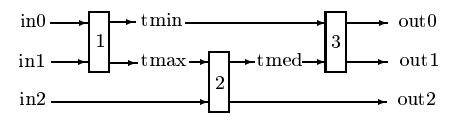
\includegraphics[width=\linewidth]{figures/sortingEx3.png}
		\caption{Mô tả về mạng sắp xếp với 3 phần tử \cite{altivec}}
		\label{fig:sortingEx3}
	\end{minipage}
	\hfill
	\begin{minipage}[b]{0.48\linewidth}
		\centering
		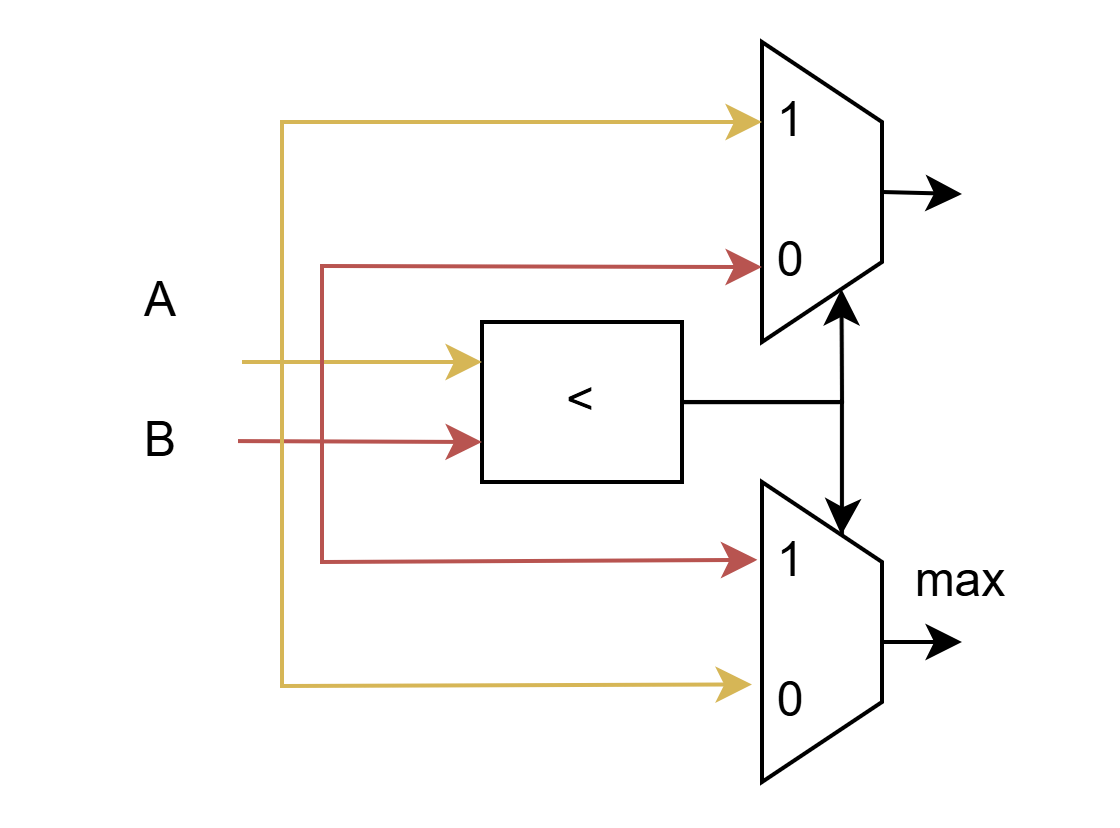
\includegraphics[width=\linewidth]{figures/node.png}
		\caption{Mô tả cấu trúc bộ so sánh và hoán đổi}
		\label{fig:node}
	\end{minipage}
\end{figure}
\subsubsection{Cửa sổ 3x3}

Hình \ref{fig:median3x3Exampel} mô tả nguyên lý và ví dụ về cách tìm giá trị trung vị của một ma trận kích thước 3x3. Với chuỗi đầu vào là 10, 9, 2, 5, 4, 3, 2, 2, 1. Giá trị trung vị ta mong đợi đạt được là 3. Các bước thực hiện bao gồm việc sắp xếp các hàng và các cột tăng dần. Sau khi đã xong hai bước trên, lúc này đường chéo gồm các phần tử 2, 4, 3. Lúc này, sẽ thực hiện sắp xếp theo thứ tự tăng dần, kết quả đạt được là 2, 3, 4. Vậy giá trị trung vị đạt được là 3, đã giống với giá trị mong đợi đạt được.  Hình \ref{fig:median3x3RTL} mô tả kiến trúc RTL của mô-đun MedianCalculation với cửa sổ 3x3. Sinh viên đã thay thế các mạng sắp xếp khi đến bước sắp xếp cột để giảm tài nguyên phần cứng sử dụng (thay bộ Sorting\_network bằng chỉ 2 Node, vì không cần đủ 3 giá trị cho bước tiếp theo), hai là đã chèn thêm các thanh ghi giữa các bước để giảm trễ lan truyền, giúp tăng tần số hoạt động của mạch.
\begin{figure}[!ht]
	\centering
	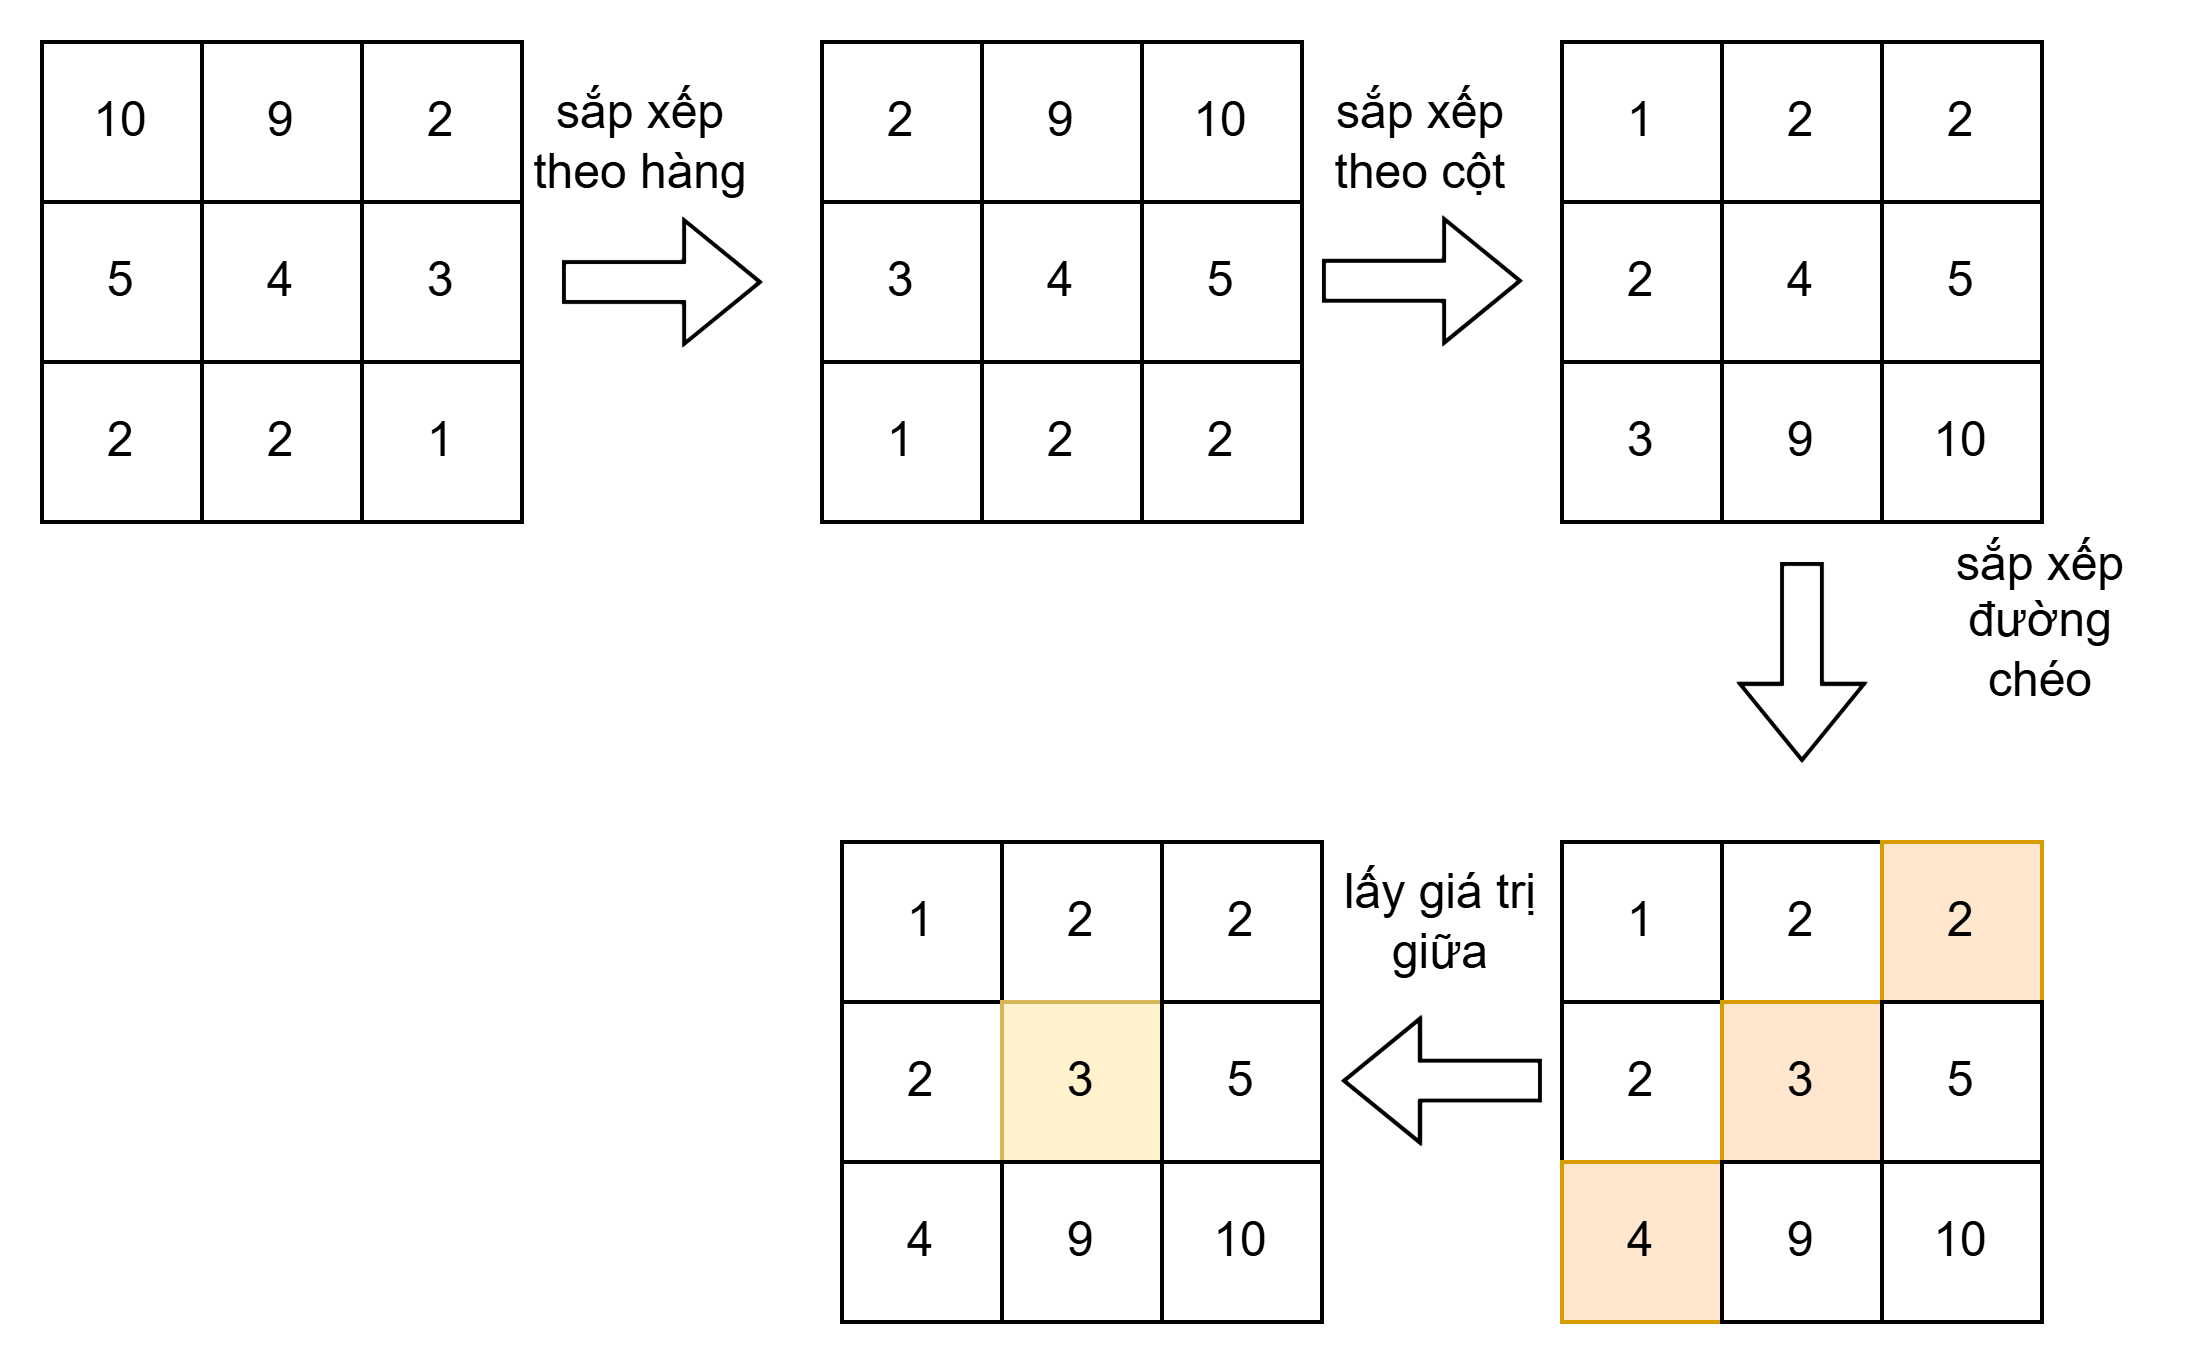
\includegraphics[width=0.6\linewidth]{figures/median3x3Exampel.png}
	\caption{Thực hiện và ví dụ của tìm trung vị của cửa sổ 3x3}
	\label{fig:median3x3Exampel}
\end{figure}
\begin{figure}[H]
	\centering
	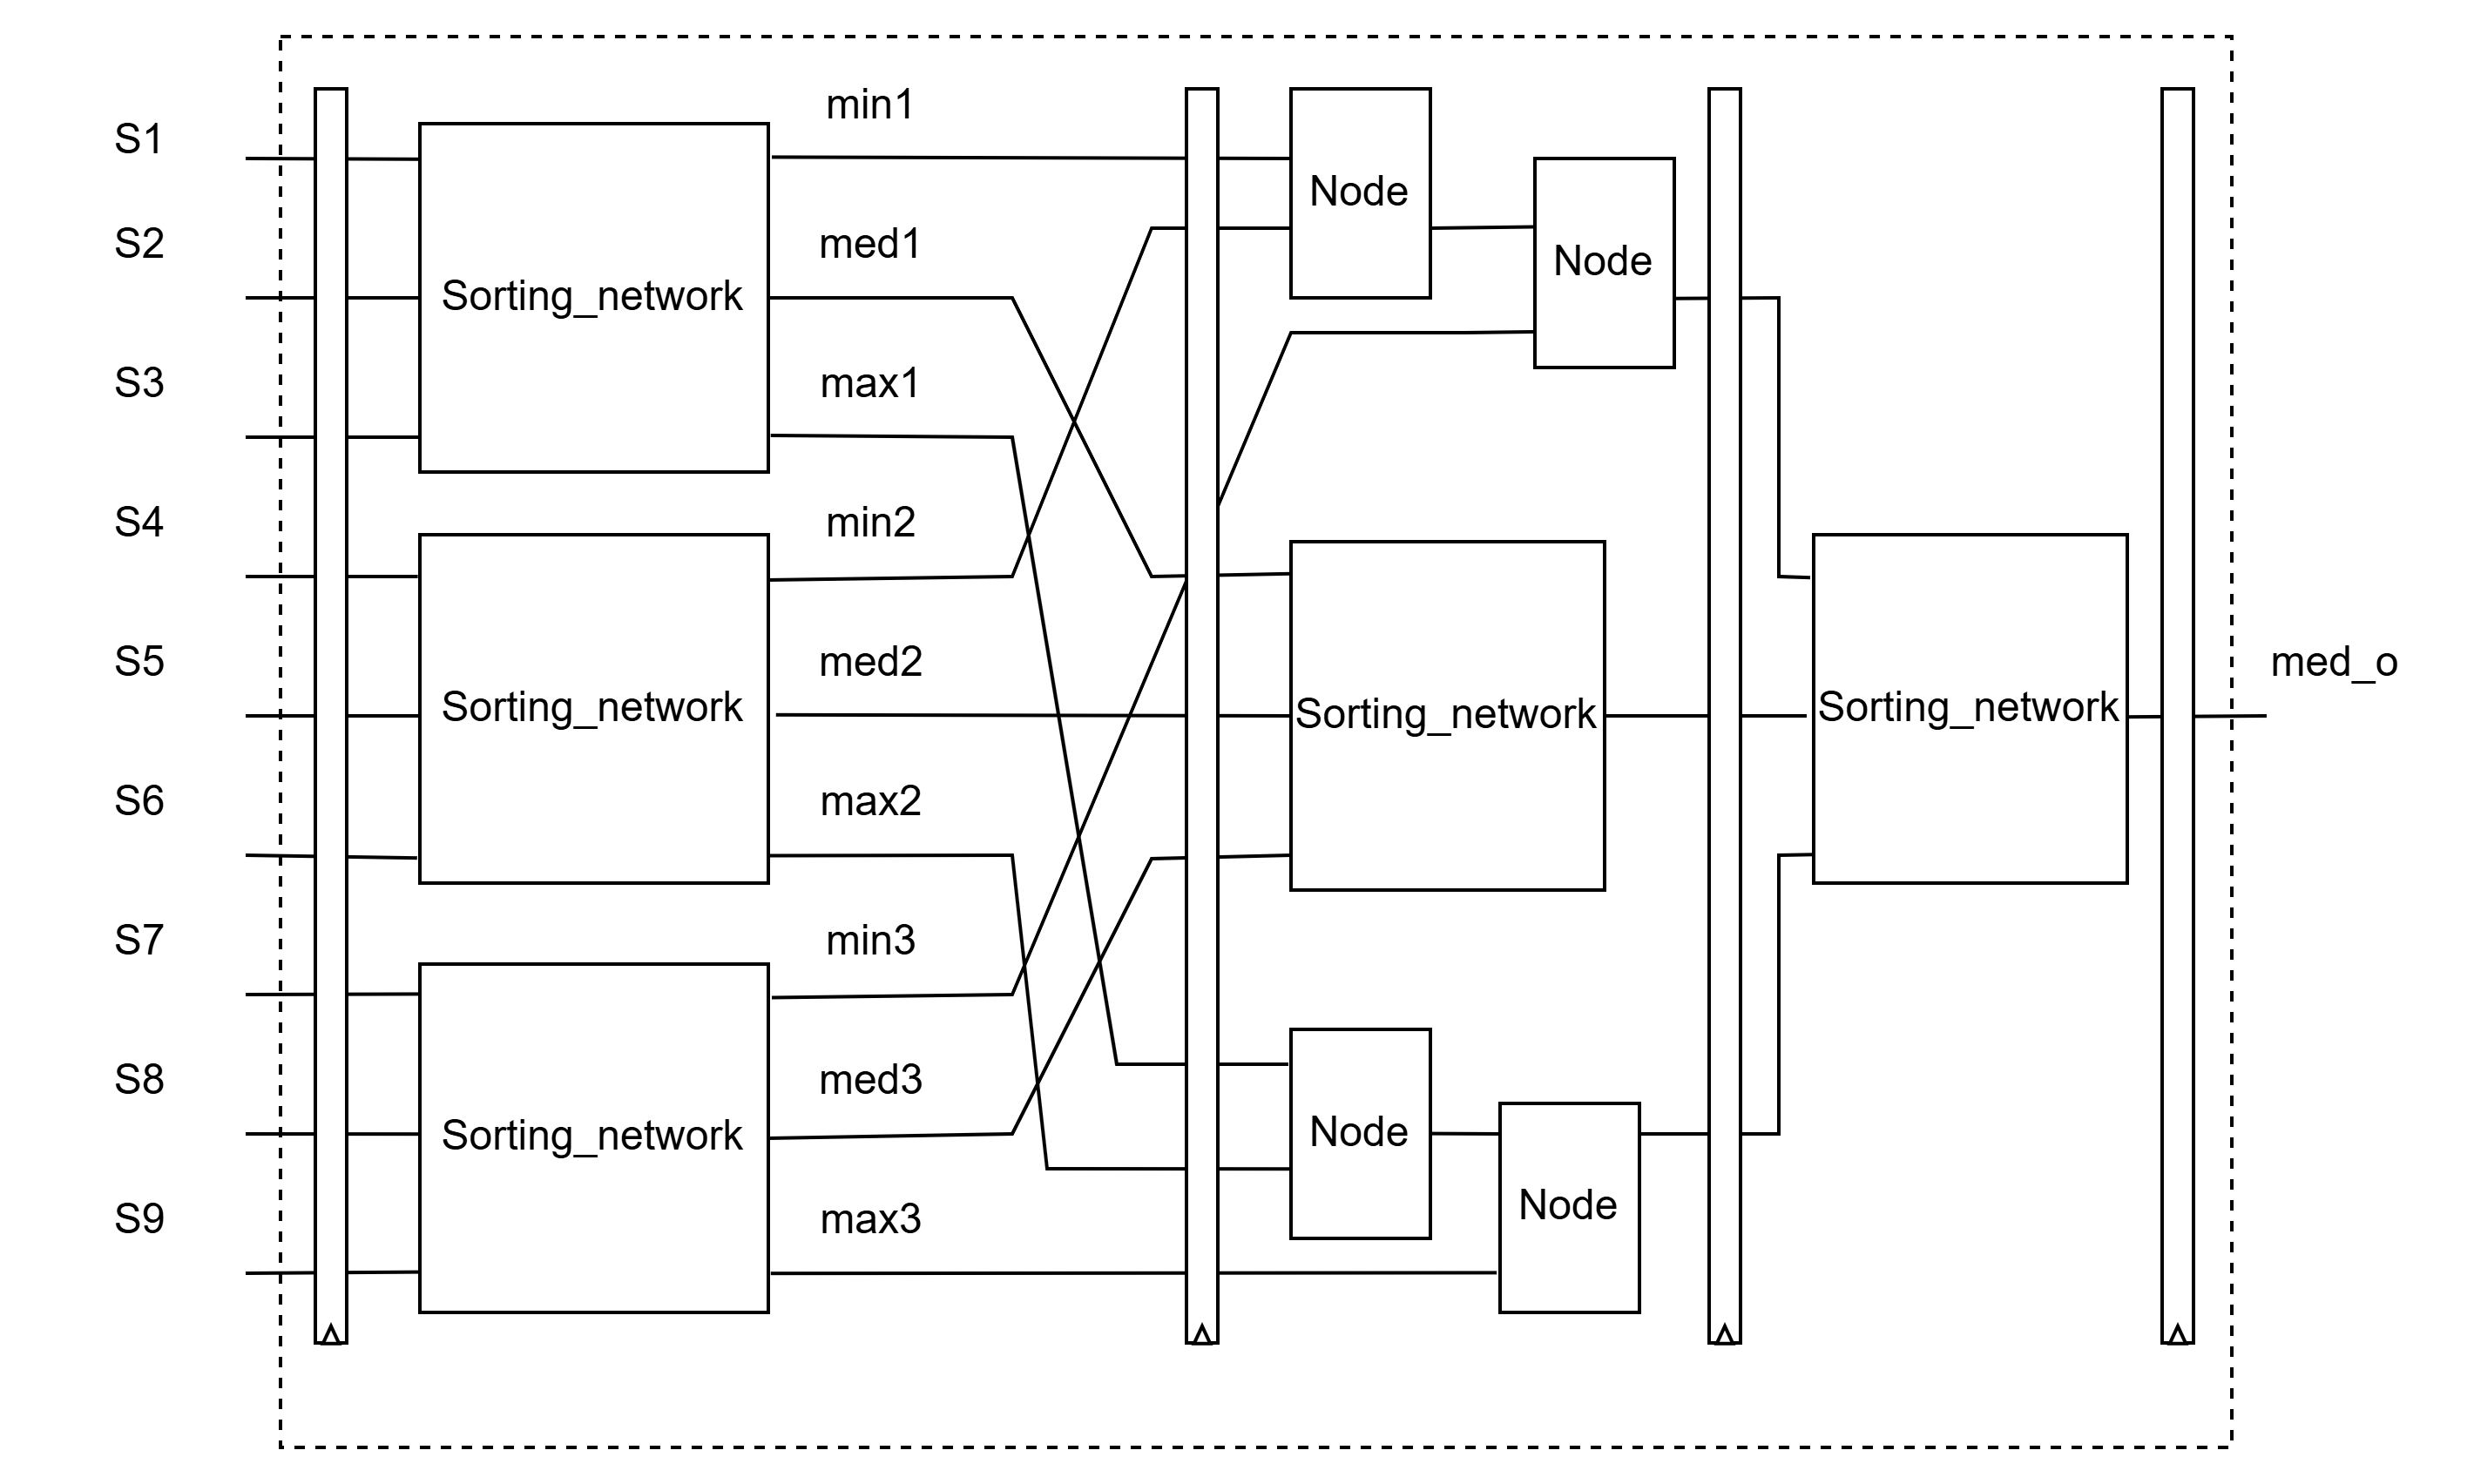
\includegraphics[width=\linewidth]{figures/median3x3RTL.png}
	\caption{Thực hiện và ví dụ của tìm trung vị của cửa sổ 3x3}
	\label{fig:median3x3RTL}
\end{figure}

\subsubsection{Cửa sổ 5x5}

Hình \ref{fig:median5x5Example} mô tả nguyên lý và ví dụ về cách tìm giá trị trung vị đối với cửa sổ 5x5. Để tối ưu cho tốc độ sắp xếp và sự không phụ thuộc, sinh viên sẽ thiết kế một sắp xếp 5 phần tử theo thứ tự tăng dần theo các bước được mô tả trong hình \ref{fig:sortAscending5x5RTL}.

\begin{figure}[!ht]
	\centering
	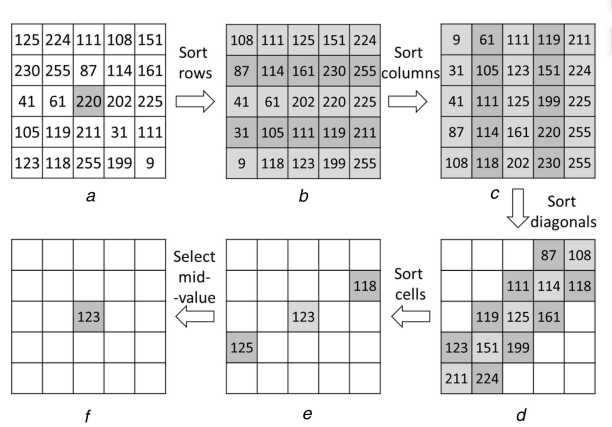
\includegraphics[width=0.8\linewidth]{figures/median5x5Example.png}
	\caption{Thực hiện và ví dụ của tìm trung vị của cửa sổ 5x5 \cite{llmf}}
	\label{fig:median5x5Example}
\end{figure}

\begin{figure}[!ht]
	\centering
	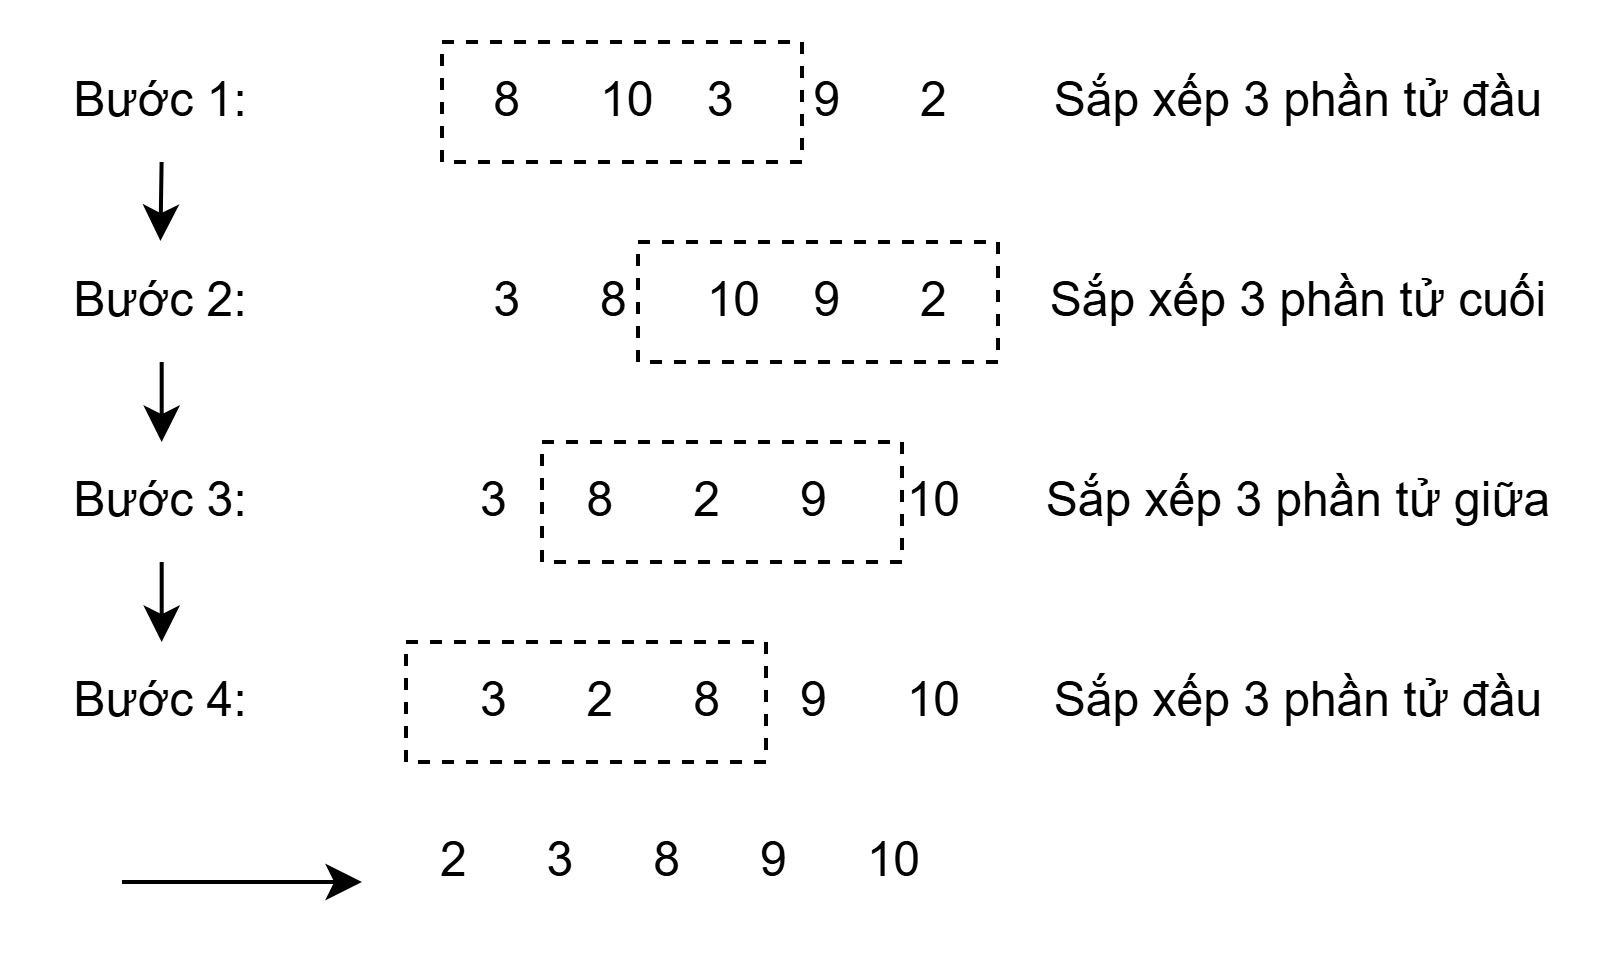
\includegraphics[width=0.8\linewidth]{figures/sortAscending5x5Ex.png}
	\caption{Xây dựng bộ sắp xếp 5 phần tử dựa trên bộ sắp xếp 3}
	\label{fig:sortAscending5x5Ex}
\end{figure}

\begin{figure}[!ht]
	\centering
	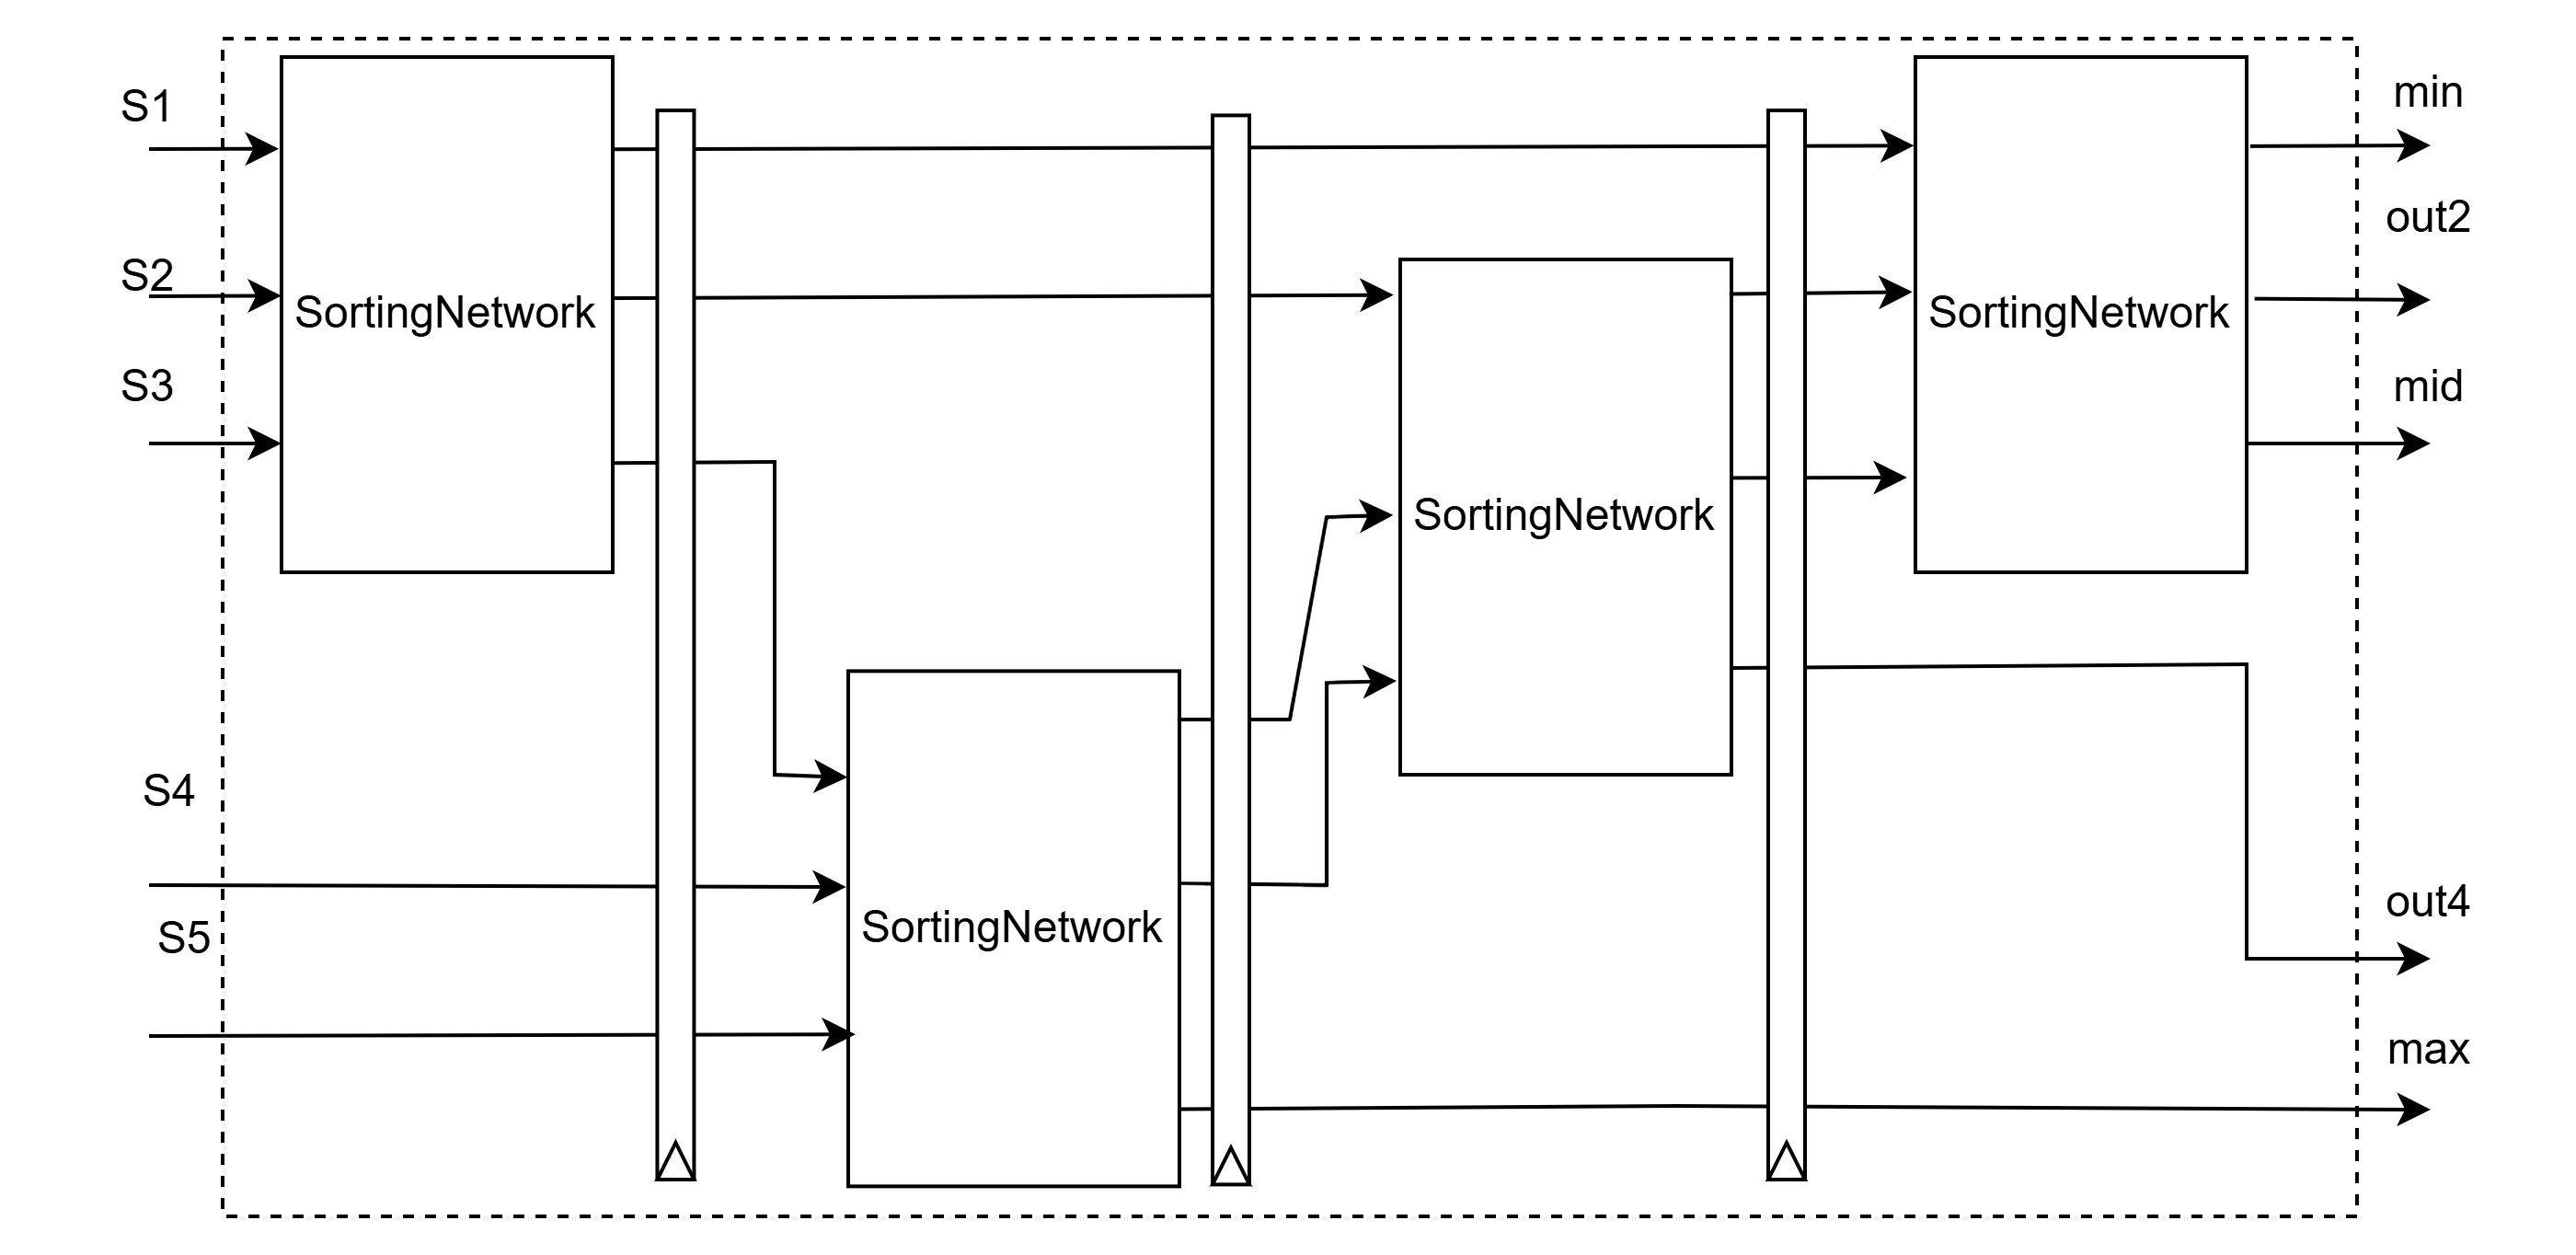
\includegraphics[width=\linewidth]{figures/sortAscending5x5RTL.png}
	\caption{Kiến trúc của bộ sắp xếp tăng dần 5 phần tử}
	\label{fig:sortAscending5x5RTL}
\end{figure}

\subsubsection{Cửa sổ 7x7}

Hình \ref{fig:median7x7Example} mô tả cách tìm ra giá trị trung vị đối với một ma trận kích thước 7x7. Điểm khác biệt đối với cửa sổ này là sau khi đã sắp xếp hàng và sắp xếp cột xong, ta sẽ tìm ra 25 phần tử thỏa mãn điều kiện, sau đó dựa vào bộ tìm trung vị đối với ma trận 5x5 để tìm trung vị chứ không thực hiện trực tiếp việc sắp xếp đường chéo theo mô tả tại thuật toán \ref{alg:medianFilterAlgo}. Sau khi sắp xếp theo hàng và cột xong, giá trị tại các ô xanh trong hình \ref{fig:median7x7Example} đã thỏa mãn điều kiện, tuy nhiên ở mỗi góc sẽ tồn tại 3 giá trị như mô tả tại ô màu vàng. Đối với phía trên, ta cần tìm giá trị lớn nhất của nó và đối với phía dưới, ta cần tìm giá trị nhỏ nhất. Từ đó, ta sẽ có đủ 25 phần tử và sử dụng nó có thể tìm kiếm được giá trị trung vị.

Để thực hiện sắp xếp tăng dần cho một cửa sổ 7x7, ta cần bộ sắp xếp tăng dần cho 7 phần tử, nó có thể được xây dựng trên các bộ sắp xếp 5 và bộ sắp xếp 3.


\begin{table}[H]
	\centering
	\renewcommand{\arraystretch}{1.3}
		\caption{Số chu kỳ thực hiện của các mô-đun mô-đun sắp xếp và mô-đun MedianCalculation}
	\begin{tabular}{|p{5cm} p{5cm} |}
		\hline
		\rowcolor{gray!30}
		\textbf{Tên mô-đun} & \textbf{Số chu kỳ}
		\\ \hline
		Bộ sắp xếp 3 phần tử & 1 chu kỳ
		  \\
		\hline
		MedianCalculation3x3  & \textbf{4 chu kỳ}
		\\ \hline
		Bộ sắp xếp 5 phần tử & 3 chu kỳ
		\\ \hline
		MedianCalculation5x5 & \textbf{14 chu kỳ}
			\\ \hline
		Bộ sắp xếp 7 phần tử & 9 chu kỳ
		\\ \hline
		MedianCalculation7x7 & \textbf{35 chu kỳ}
		\\ \hline
	\end{tabular}

	\label{tab:numberOfCycleMedianCalculation}
\end{table}

\begin{figure}[!ht]
	\centering
	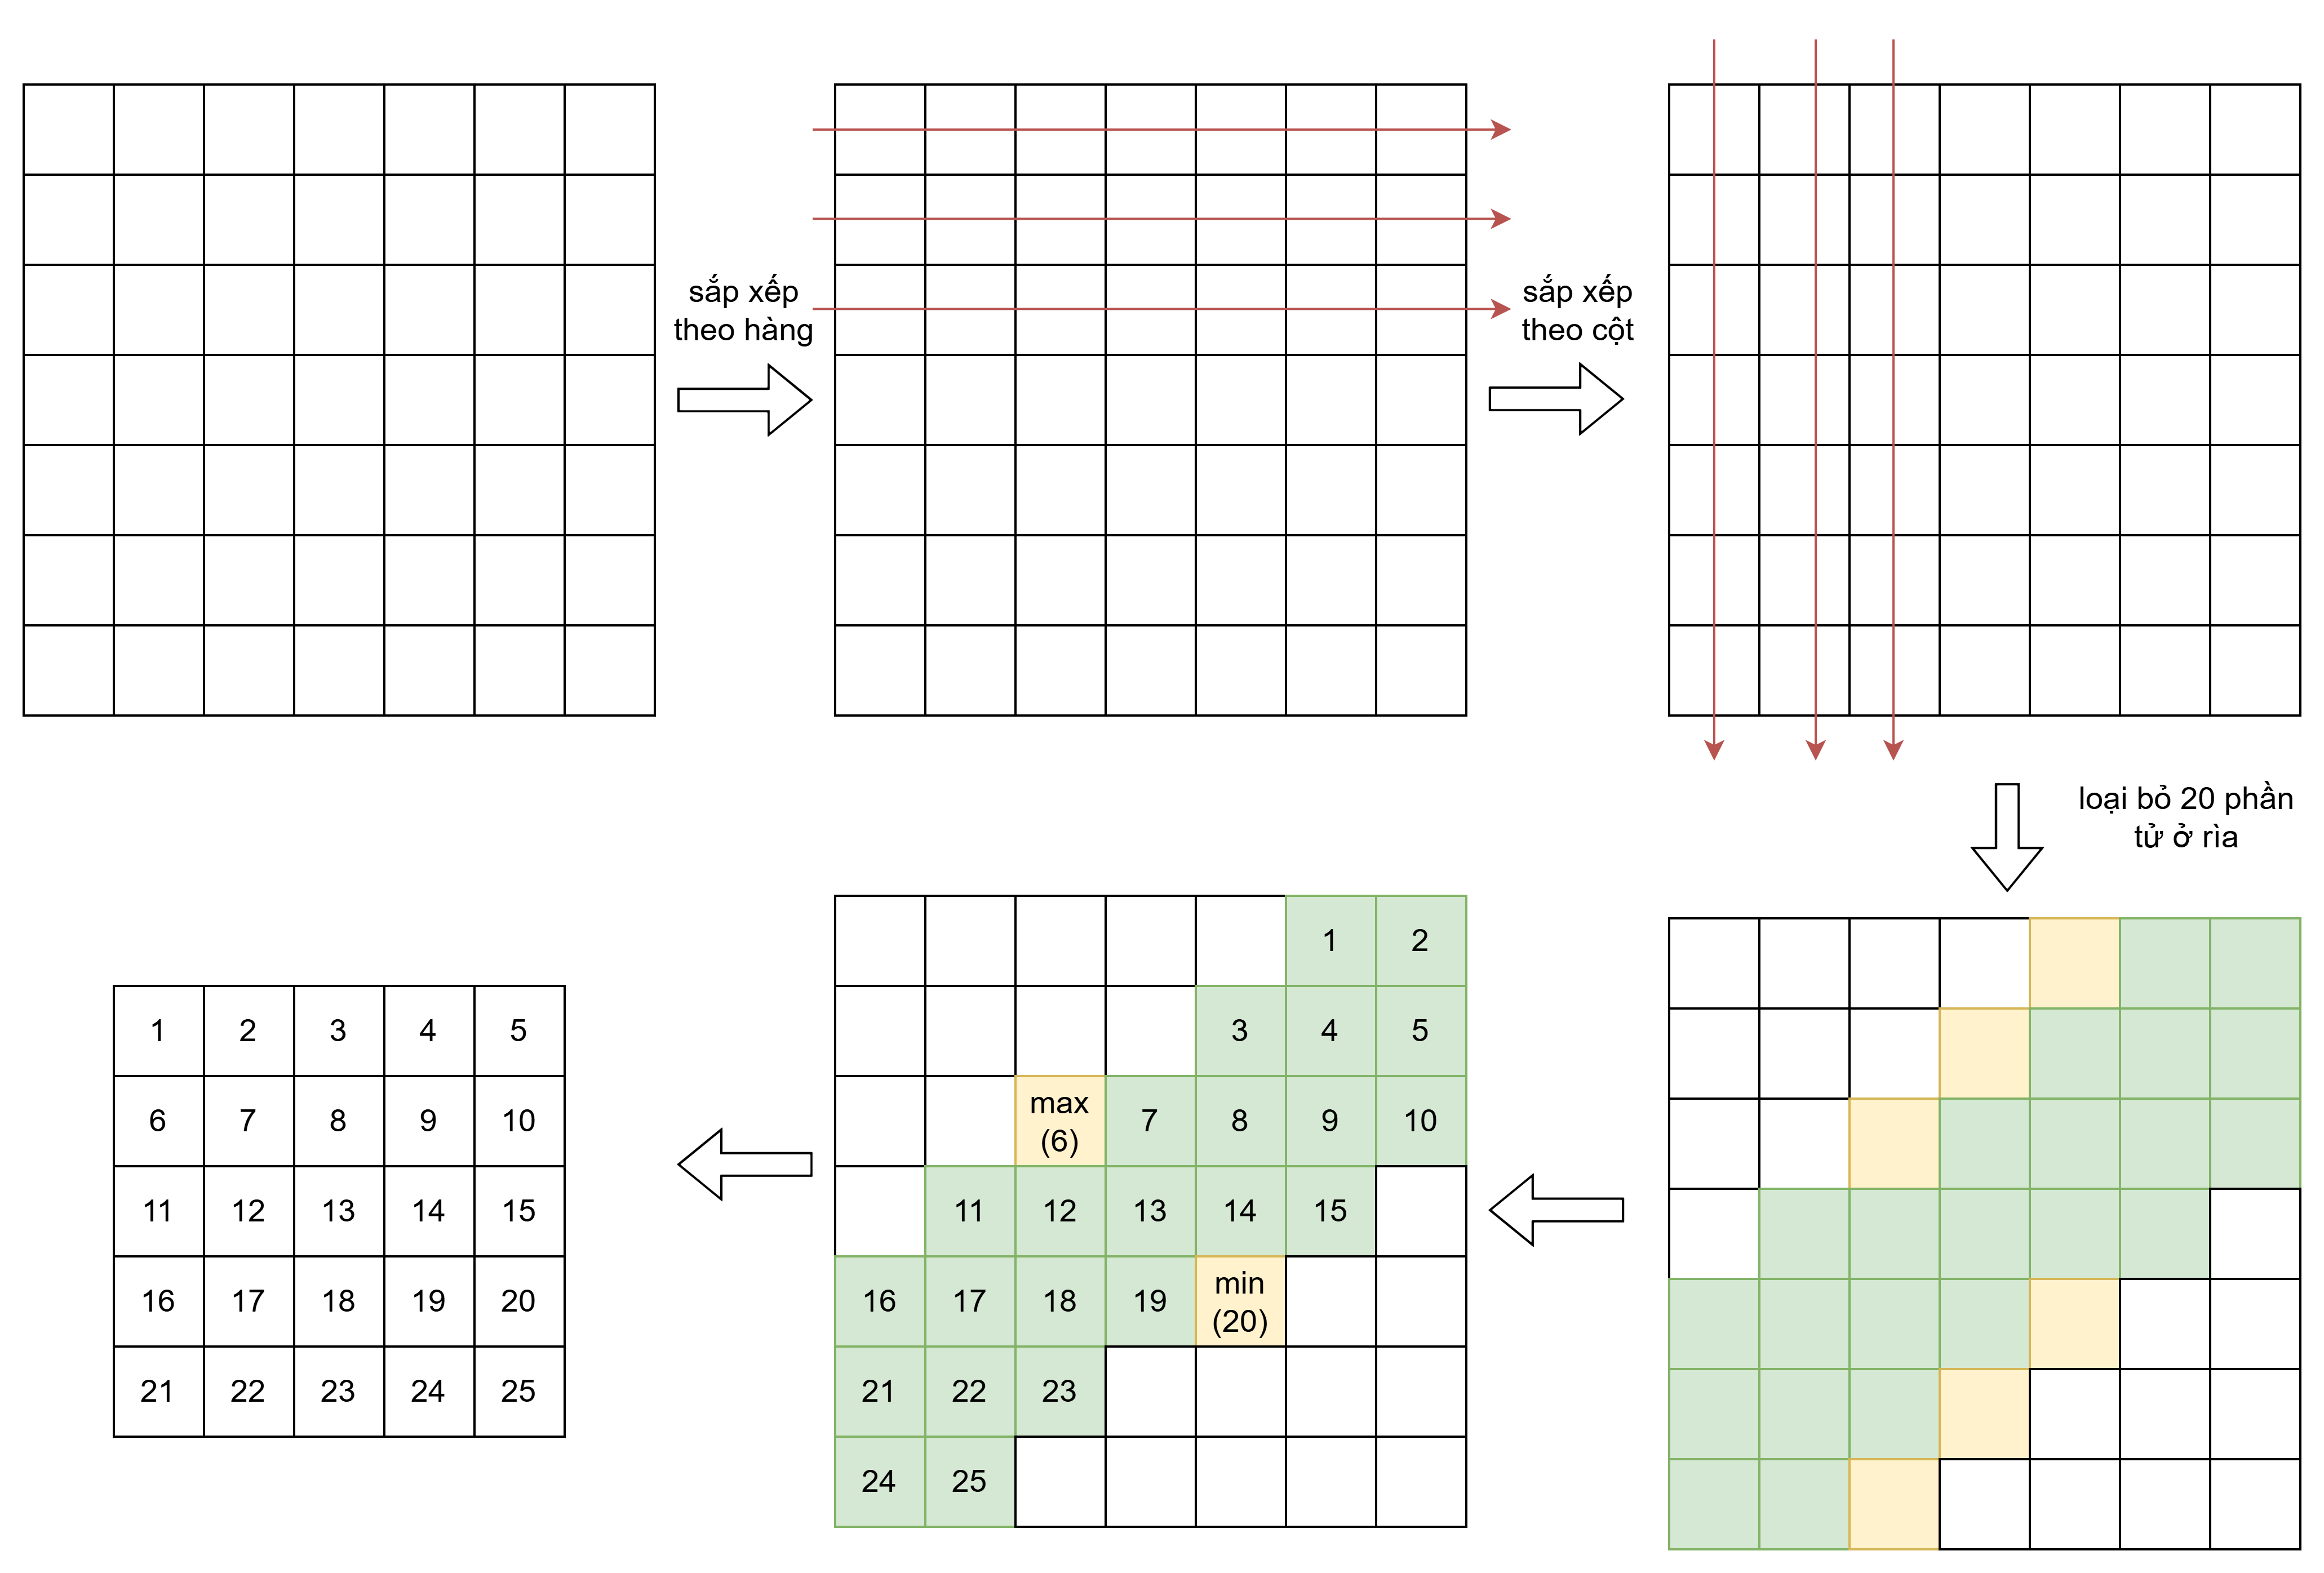
\includegraphics[width=\linewidth]{figures/median7x7Example.png}
	\caption{Thực hiện và ví dụ của tìm trung vị của cửa sổ 7x7}
	\label{fig:median7x7Example}
\end{figure}
\begin{figure}[!ht]
	\centering
	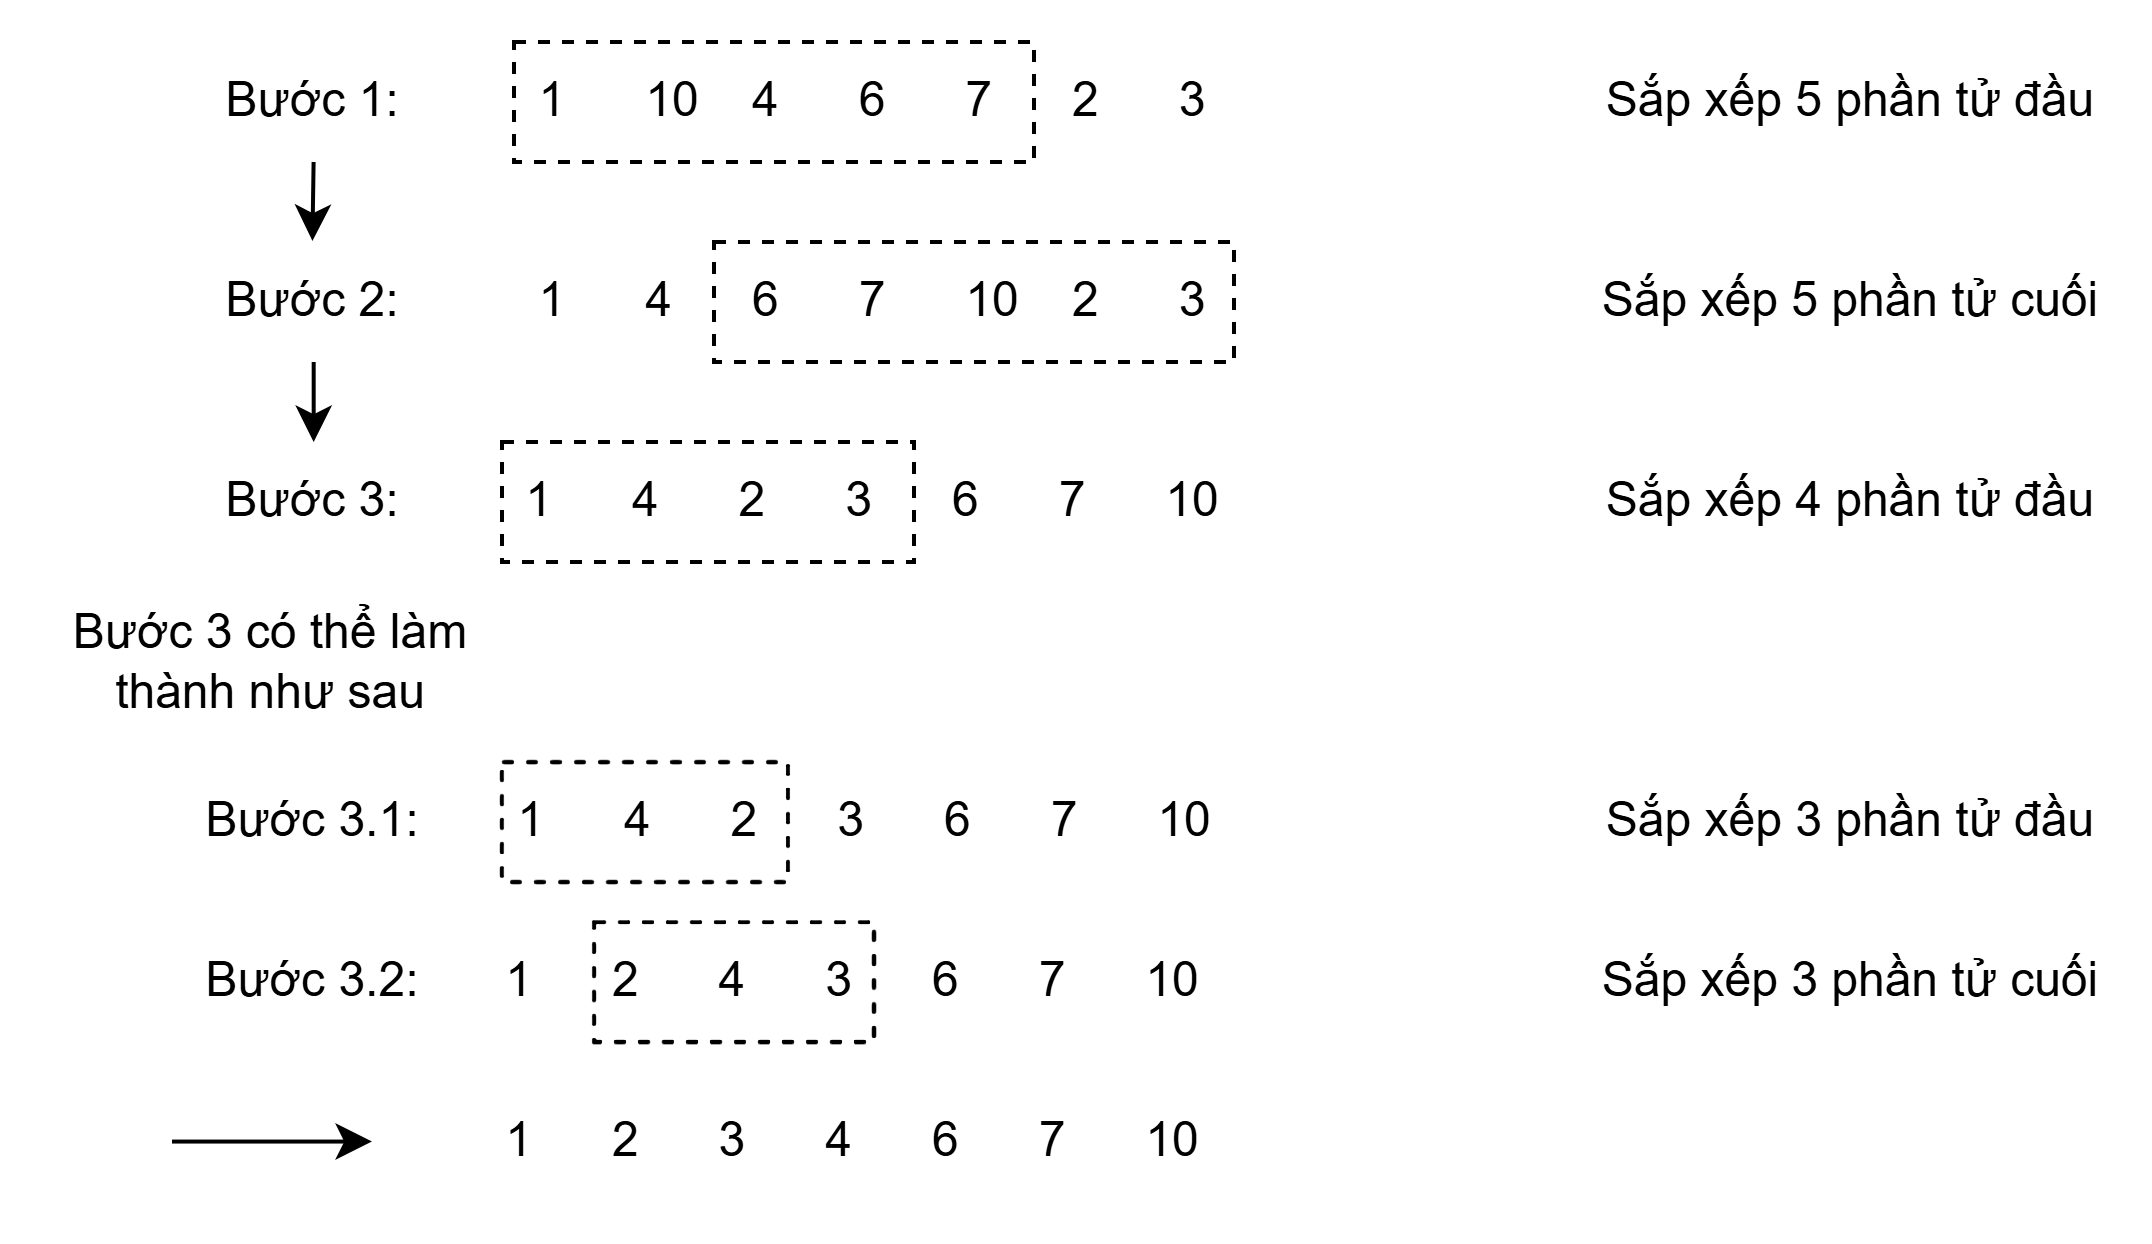
\includegraphics[width=0.8\linewidth]{figures/sortAscending7x7Ex.png}
	\caption{Xây dựng bộ sắp xếp 7 phần tử dựa trên bộ sắp xếp 5 và bộ sắp xếp 3}
	\label{fig:sortAscending7x7Ex}
\end{figure}

\section{mô-đun CI}
mô-đun CI thực chất là tập hợp của các 3 mô-đun MRELBP\_CI, trong mỗi mô-đun đó là khối PatchSum nối với một mạch logic tổ hợp để nhằm mục đích so sánh và đưa ra giá trị so sánh đối với các phần tử trung tâm của một cửa sổ. Về cơ bản 3 mô-đun PatchSum đều xây dựng trên nguyên tắc chung sẽ được trình bày tại phần ngay sau.
\subsection{Cơ sở xây dựng mô-đun PatchSum}
Một cách đơn giản nhất để tính tổng của các cửa sổ là cộng tất cả các giá trị trong cửa sổ lại với nhau, nếu với cửa sổ kích thước 5x5, ta sẽ cần cộng khoảng 25 giá trị trong 1 chu kỳ (nếu không sử dụng phương pháp đường ống), hoặc thực hiện một bộ cộng tuần tự, tuy nhiên nó sẽ giảm khả năng xử lý thời gian thực. Để giải quyết vấn đề này, sinh viên sẽ thực hiện một kỹ thuật triển khai giống với cửa sổ trượt. Hình \ref{fig:slidingWindowPrincipla} mô tả một ví dụ về kỹ thuật cửa sổ trượt. Cửa sổ mà có viền màu đỏ là cửa sổ ban đầu. Cửa sổ mà có viền màu xanh là cửa sổ ngay sau cửa sổ màu đỏ. Ta thấy, tổng của 2 cửa sổ này đều có một đặc điểm là có các giá trị ở các ô màu vàng. Giá trị tổng của cửa sổ sau sẽ bằng giá trị của cửa sổ trước đó trừ đi giá trị ở các ô màu đỏ và cộng với các giá trị ở các ô màu xanh. Bằng nguyên lý đó, ta có thể giảm bớt số lượng phép cộng cần thực hiện trong 1 chu kỳ.


\begin{figure}[!ht]
	\centering
	\begin{minipage}[t]{0.48\linewidth}
		\centering
		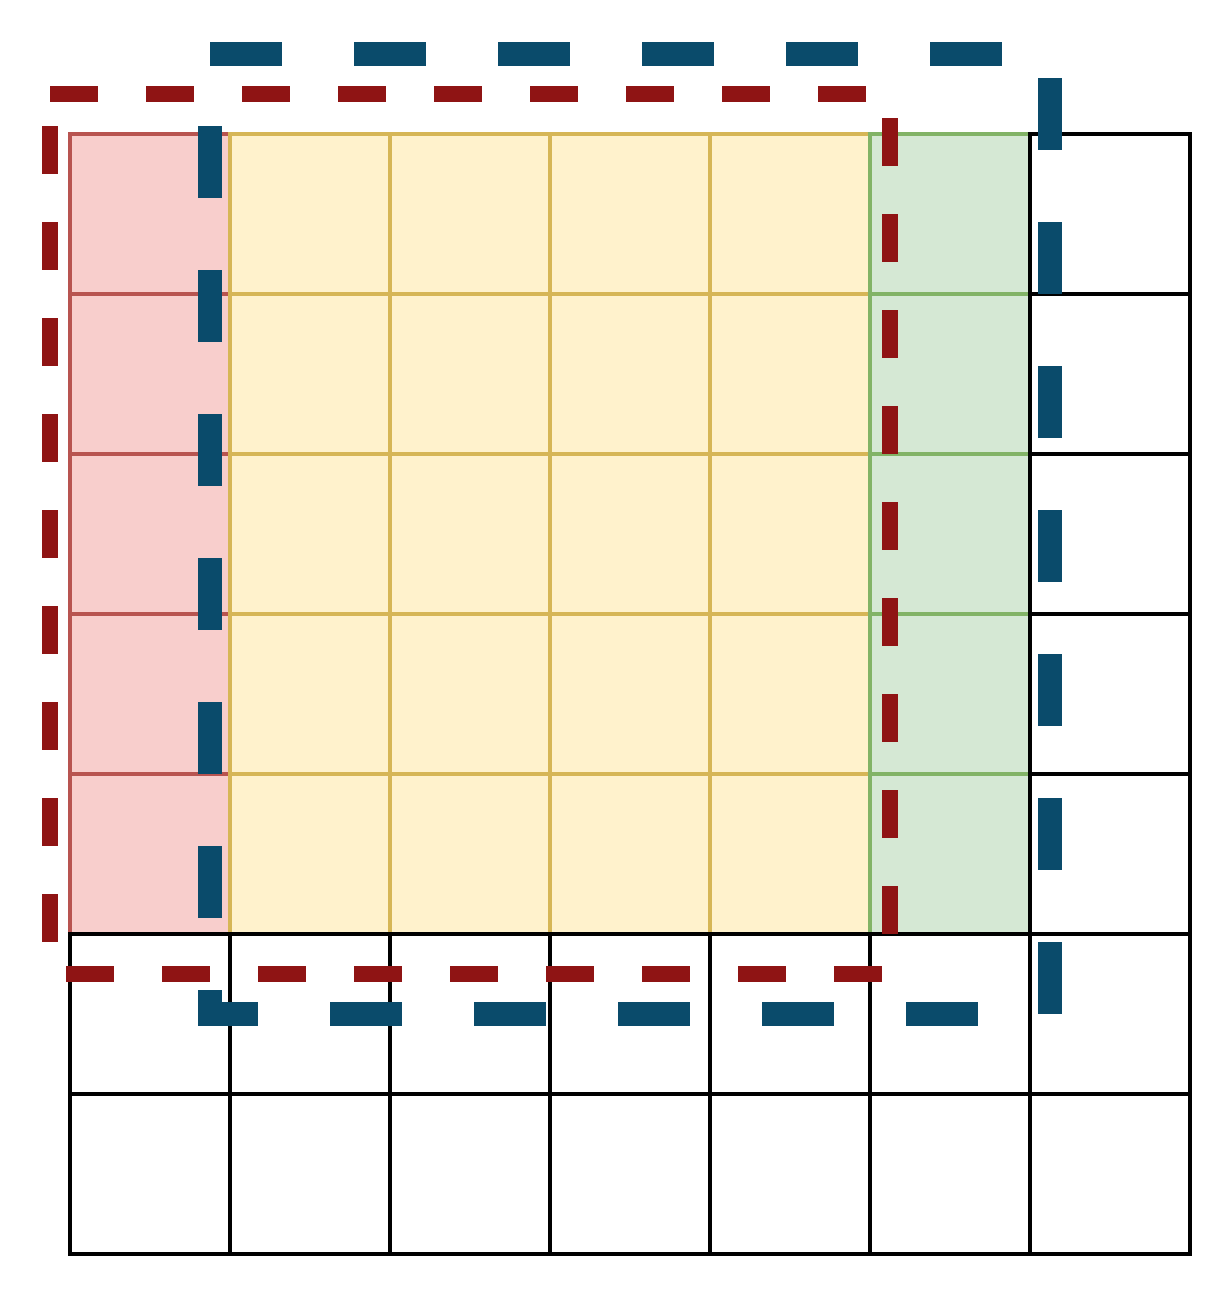
\includegraphics[width=\linewidth]{figures/slidingWindowPrincipla.png}
		\caption{Ví dụ về nguyên lý cửa kỹ thuật cửa sổ trượt}
		\label{fig:slidingWindowPrincipla}
	\end{minipage}
	\hfill
	\begin{minipage}[t]{0.48\linewidth}
		\centering
		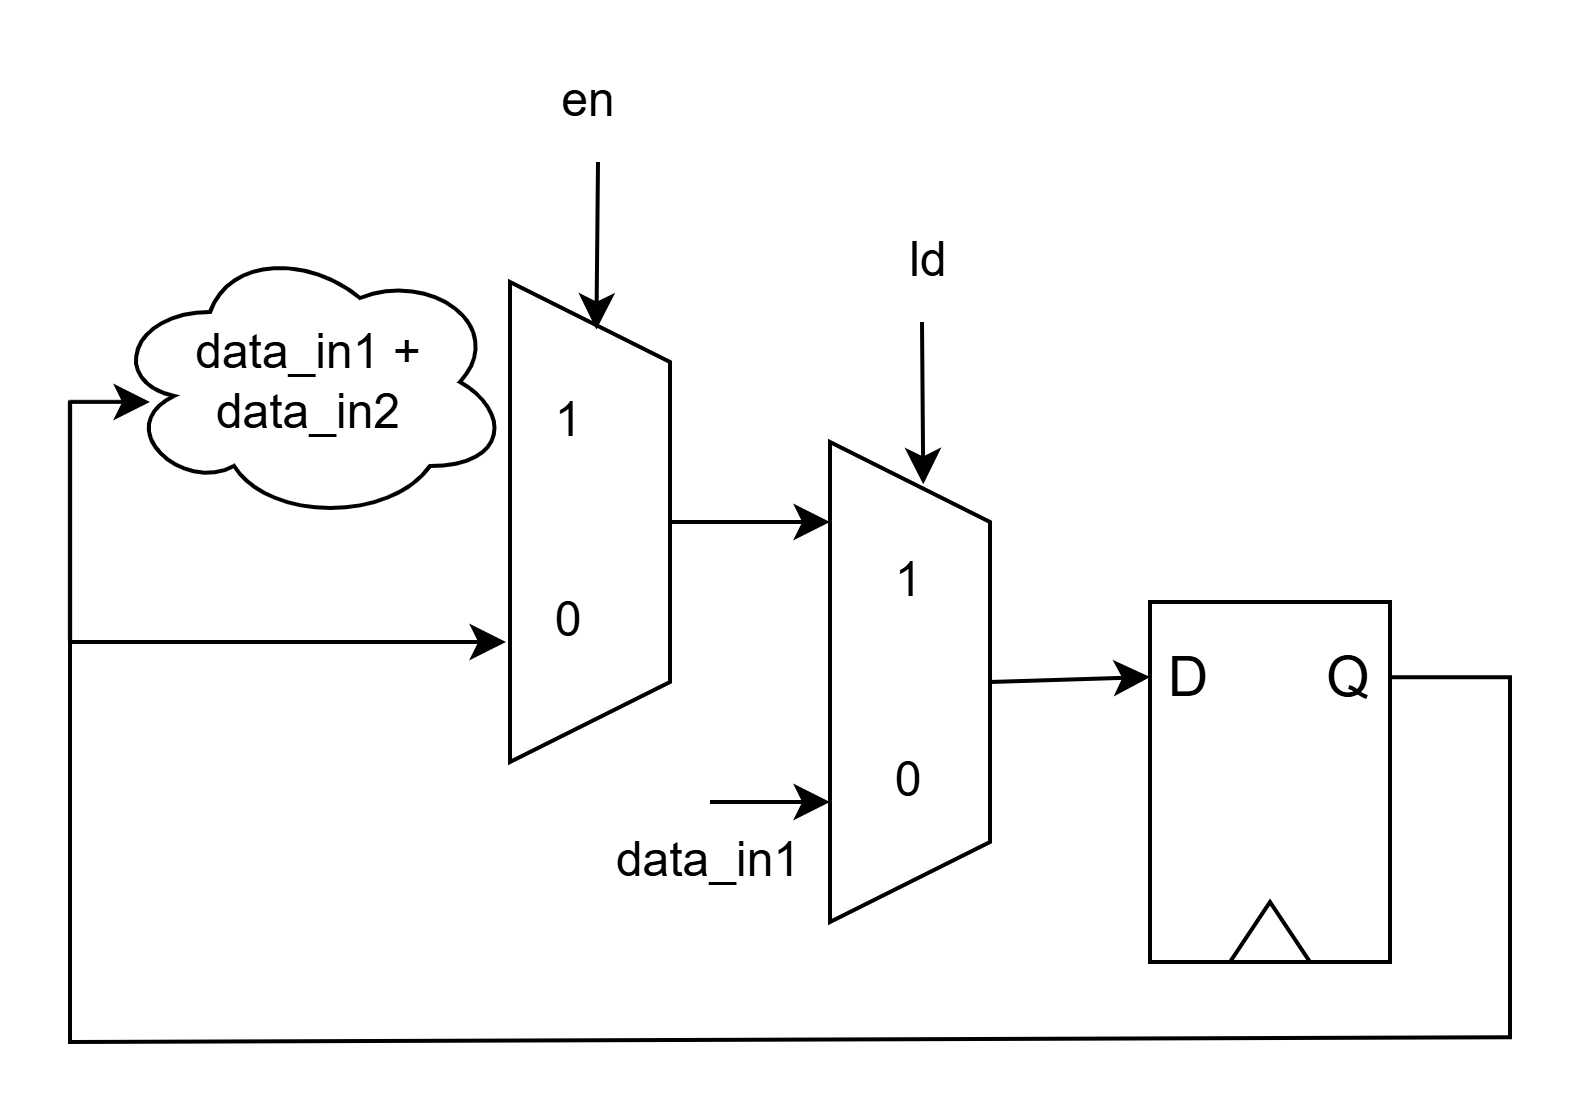
\includegraphics[width=\linewidth]{figures/sumCumRTL.png}
		\caption{Kiến trúc của mô-đun sum\_cum}
		\label{fig:sumCumRTL}
	\end{minipage}
\end{figure}



\subsection{Xây dựng mô-đun PatchSum}
\subsubsection{Sơ đồ chuyển trạng thái}
Vì sẽ xây dựng 3 mô-đun PatchSum ứng với 3 giá trị bán kính r khác nhau, tuy nhiên cả 3 mô-đun này đều có cùng 1 nguyên lý hoạt động, do đó sinh viên sẽ xây dựng chung 1 bộ sơ đồ chuyển trạng thái, được mô tả tại hình \ref{fig:patchSumTrans}. 

\begin{figure}[!ht]
	\centering
	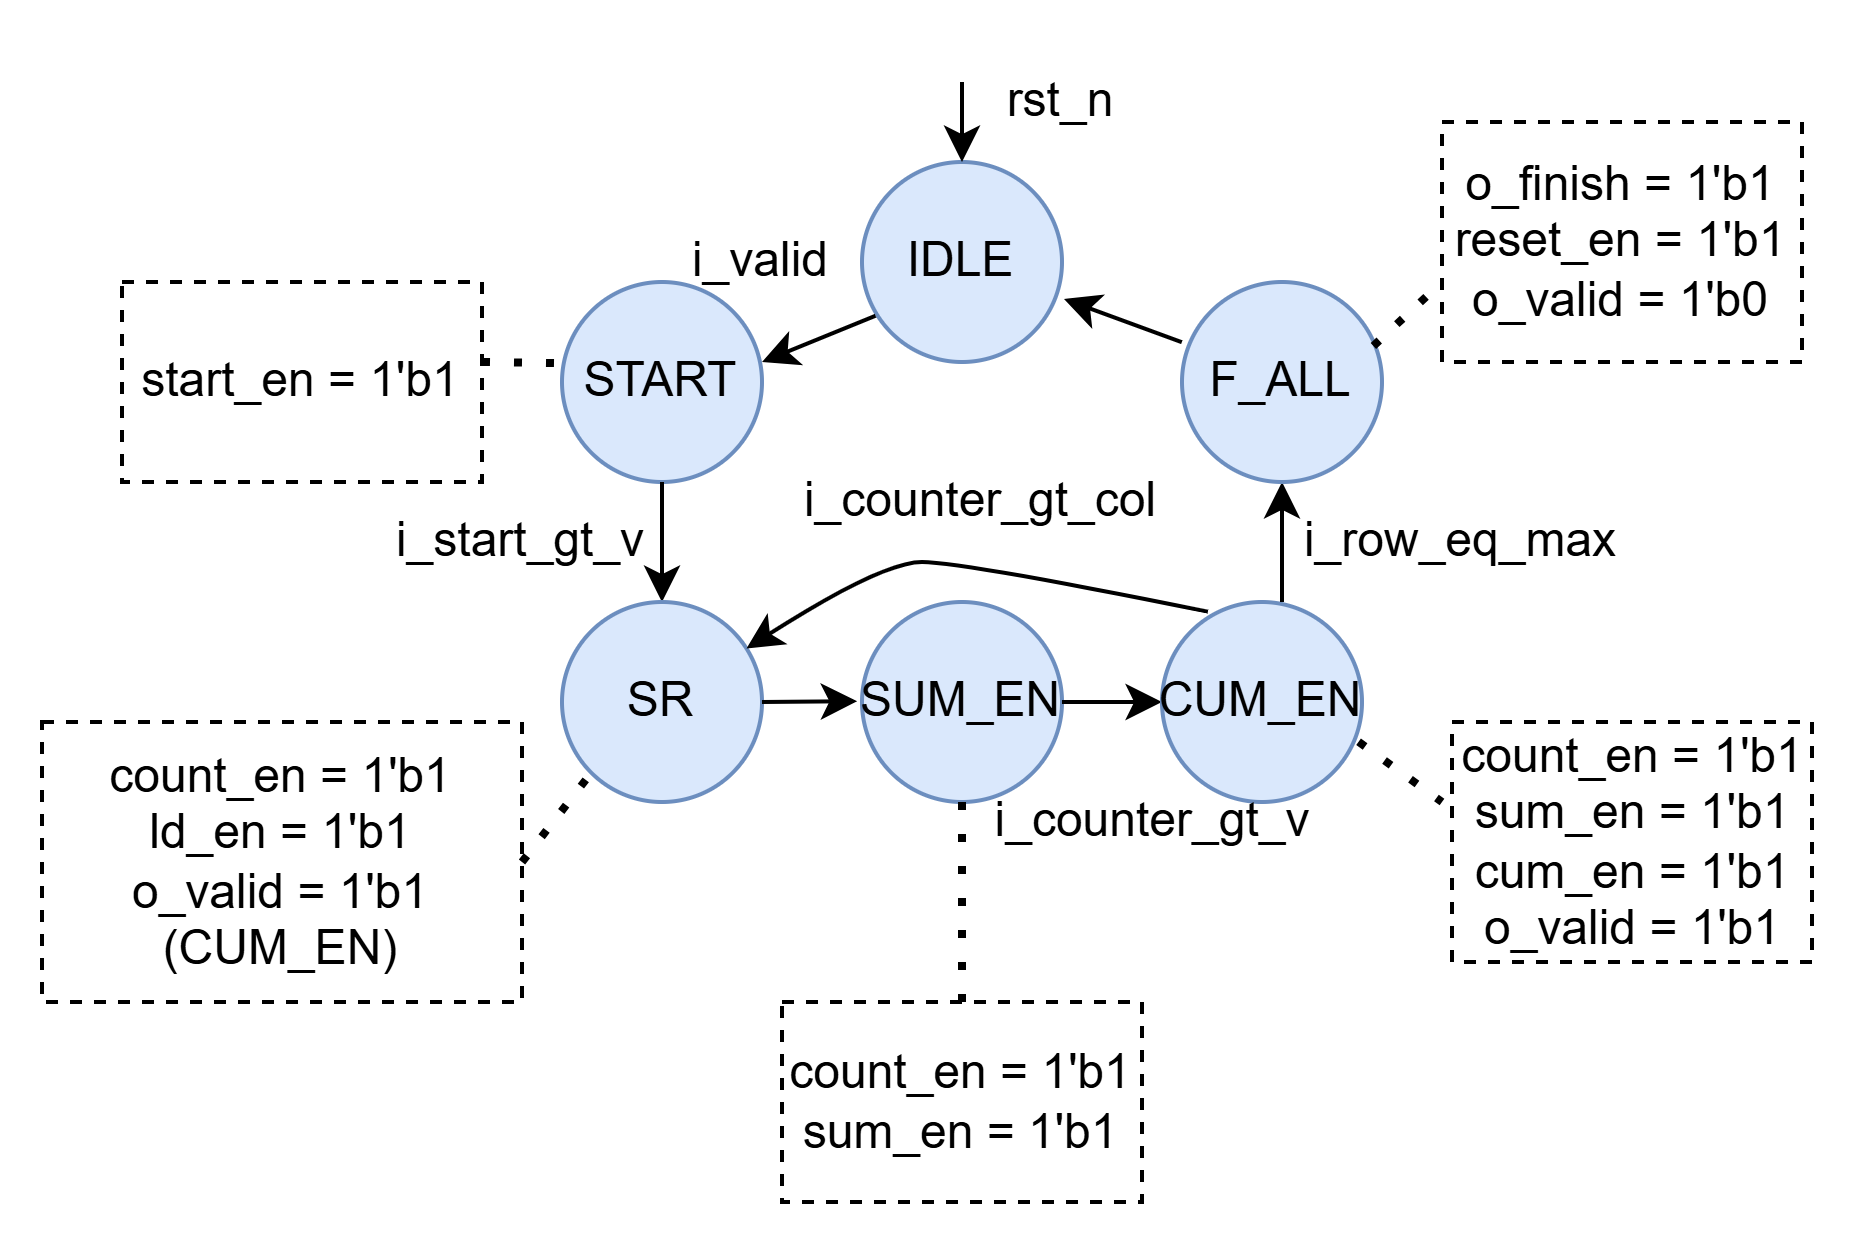
\includegraphics[width=0.8\linewidth]{figures/patchSumTrans.png}
	\caption{Sơ đồ chuyển trạng thái của mô-đun PatchSum}
	\label{fig:patchSumTrans}
\end{figure}
\subsubsection{Kiến trúc RTL}
Hình \ref{fig:patchSumRTL} mô tả kiến trúc RTL chung của cả 3 bộ PatchSum ứng với các bán kính r = 2, 4, 6. Đây là các bộ giúp kiểm tra các điều kiện để máy trạng thái chuyển trạng thái, cả 3 mô-đun ứng với 3 loại r khác nhau đều sử dụng các bộ này, tuy nhiên thì mỗi bán kính sẽ ứng với các điều kiện khác nhau và các điều kiện Condition sẽ được mô tả tại bảng \ref{tab:conditionRTLPatchSum}. Một mô PatchSum ứng với một giá trị r cụ thể sẽ có mô tả RTL ở cả 2 hình \ref{fig:patchSumRTL} và \ref{fig:patchSumRTL_2}. Tuy nhiên hình \ref{fig:patchSumRTL_2} là mô tả RTL đầu ra cho mô-đun PatchSum với r = 2, với r = 4 và r = 6, kiến trúc sẽ có sự khác biệt về số lượng thanh ghi, số chu kỳ thực hiện, nhưng về nguyên lý hoạt động là tương tự nhau. Hình \ref{fig:sumCumRTL} mô tả cấu trúc của mô-đun sum\_cum được sử dụng ở cuối kiến trúc RTL (2) của mô-đun PatchSum.
\begin{table}[H]
	\centering
		\caption{Bảng điều kiện cho mô tả hình \ref{fig:patchSumRTL}}
	\begin{tabular}{|>{\centering\arraybackslash}m{5cm}|>{\centering\arraybackslash}m{3cm}|>{\centering\arraybackslash}m{3cm}|>{\centering\arraybackslash}m{3cm}|}
		\hline
		\rowcolor{gray!30}
		\diagbox[width=5cm,height=1.5cm,dir=NE]{\textbf{Loại điều kiện}}{\textbf{Bán kính}} & \textbf{r = 2}  & \textbf{r = 4} & \textbf{r = 6} \\
		\hline
		Condition1 & > 3 & > 7 & > 11 \\
		\hline
		Condition2 & COLS - 2 & COLS - 2 & COLS - 2 \\
		\hline
		Condition3 & > 1 & > 2 & > 2 \\
		\hline
		Condition4 & ROWS - 4 & ROWS - 8 & ROWS - 12 \\
		\hline
	\end{tabular}

	\label{tab:conditionRTLPatchSum}
\end{table}

\begin{figure}[!ht]
	\centering
	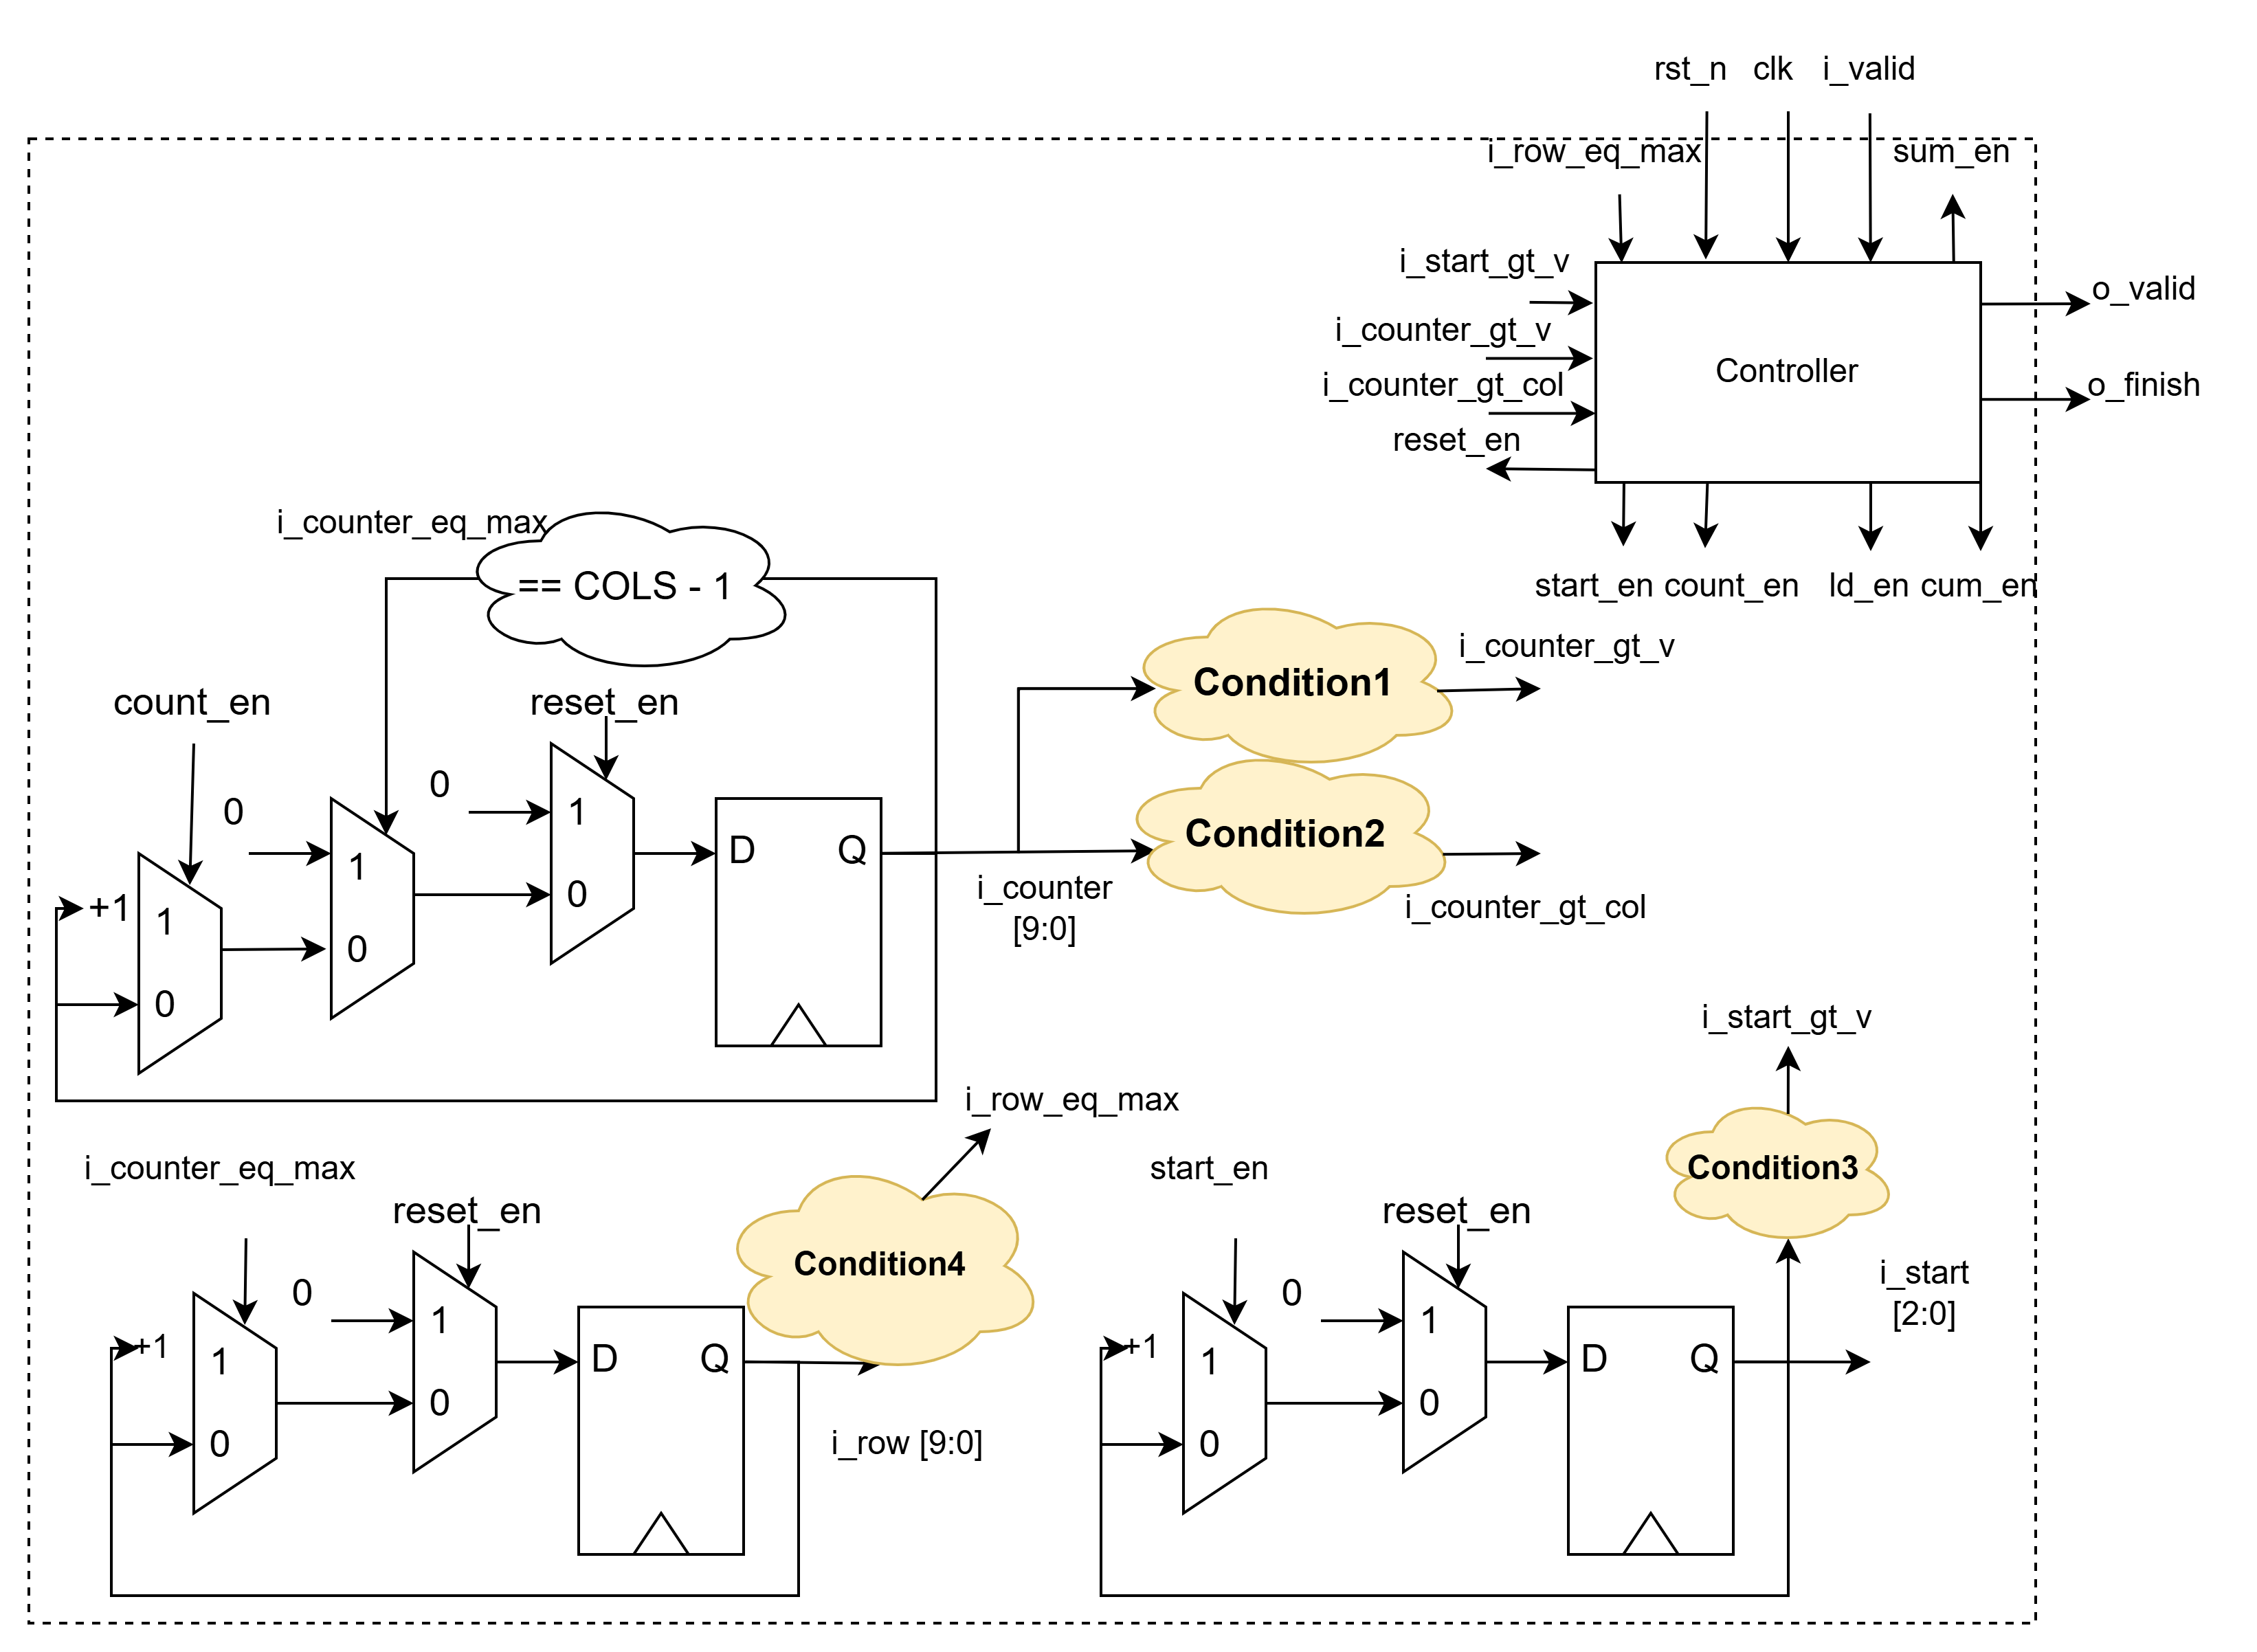
\includegraphics[width=\linewidth]{figures/patchSumRTL.png}
	\caption{Kiến trúc RTL (1) của mô-đun PatchSum}
	\label{fig:patchSumRTL}
\end{figure}
\begin{figure}[!ht]
	\centering
	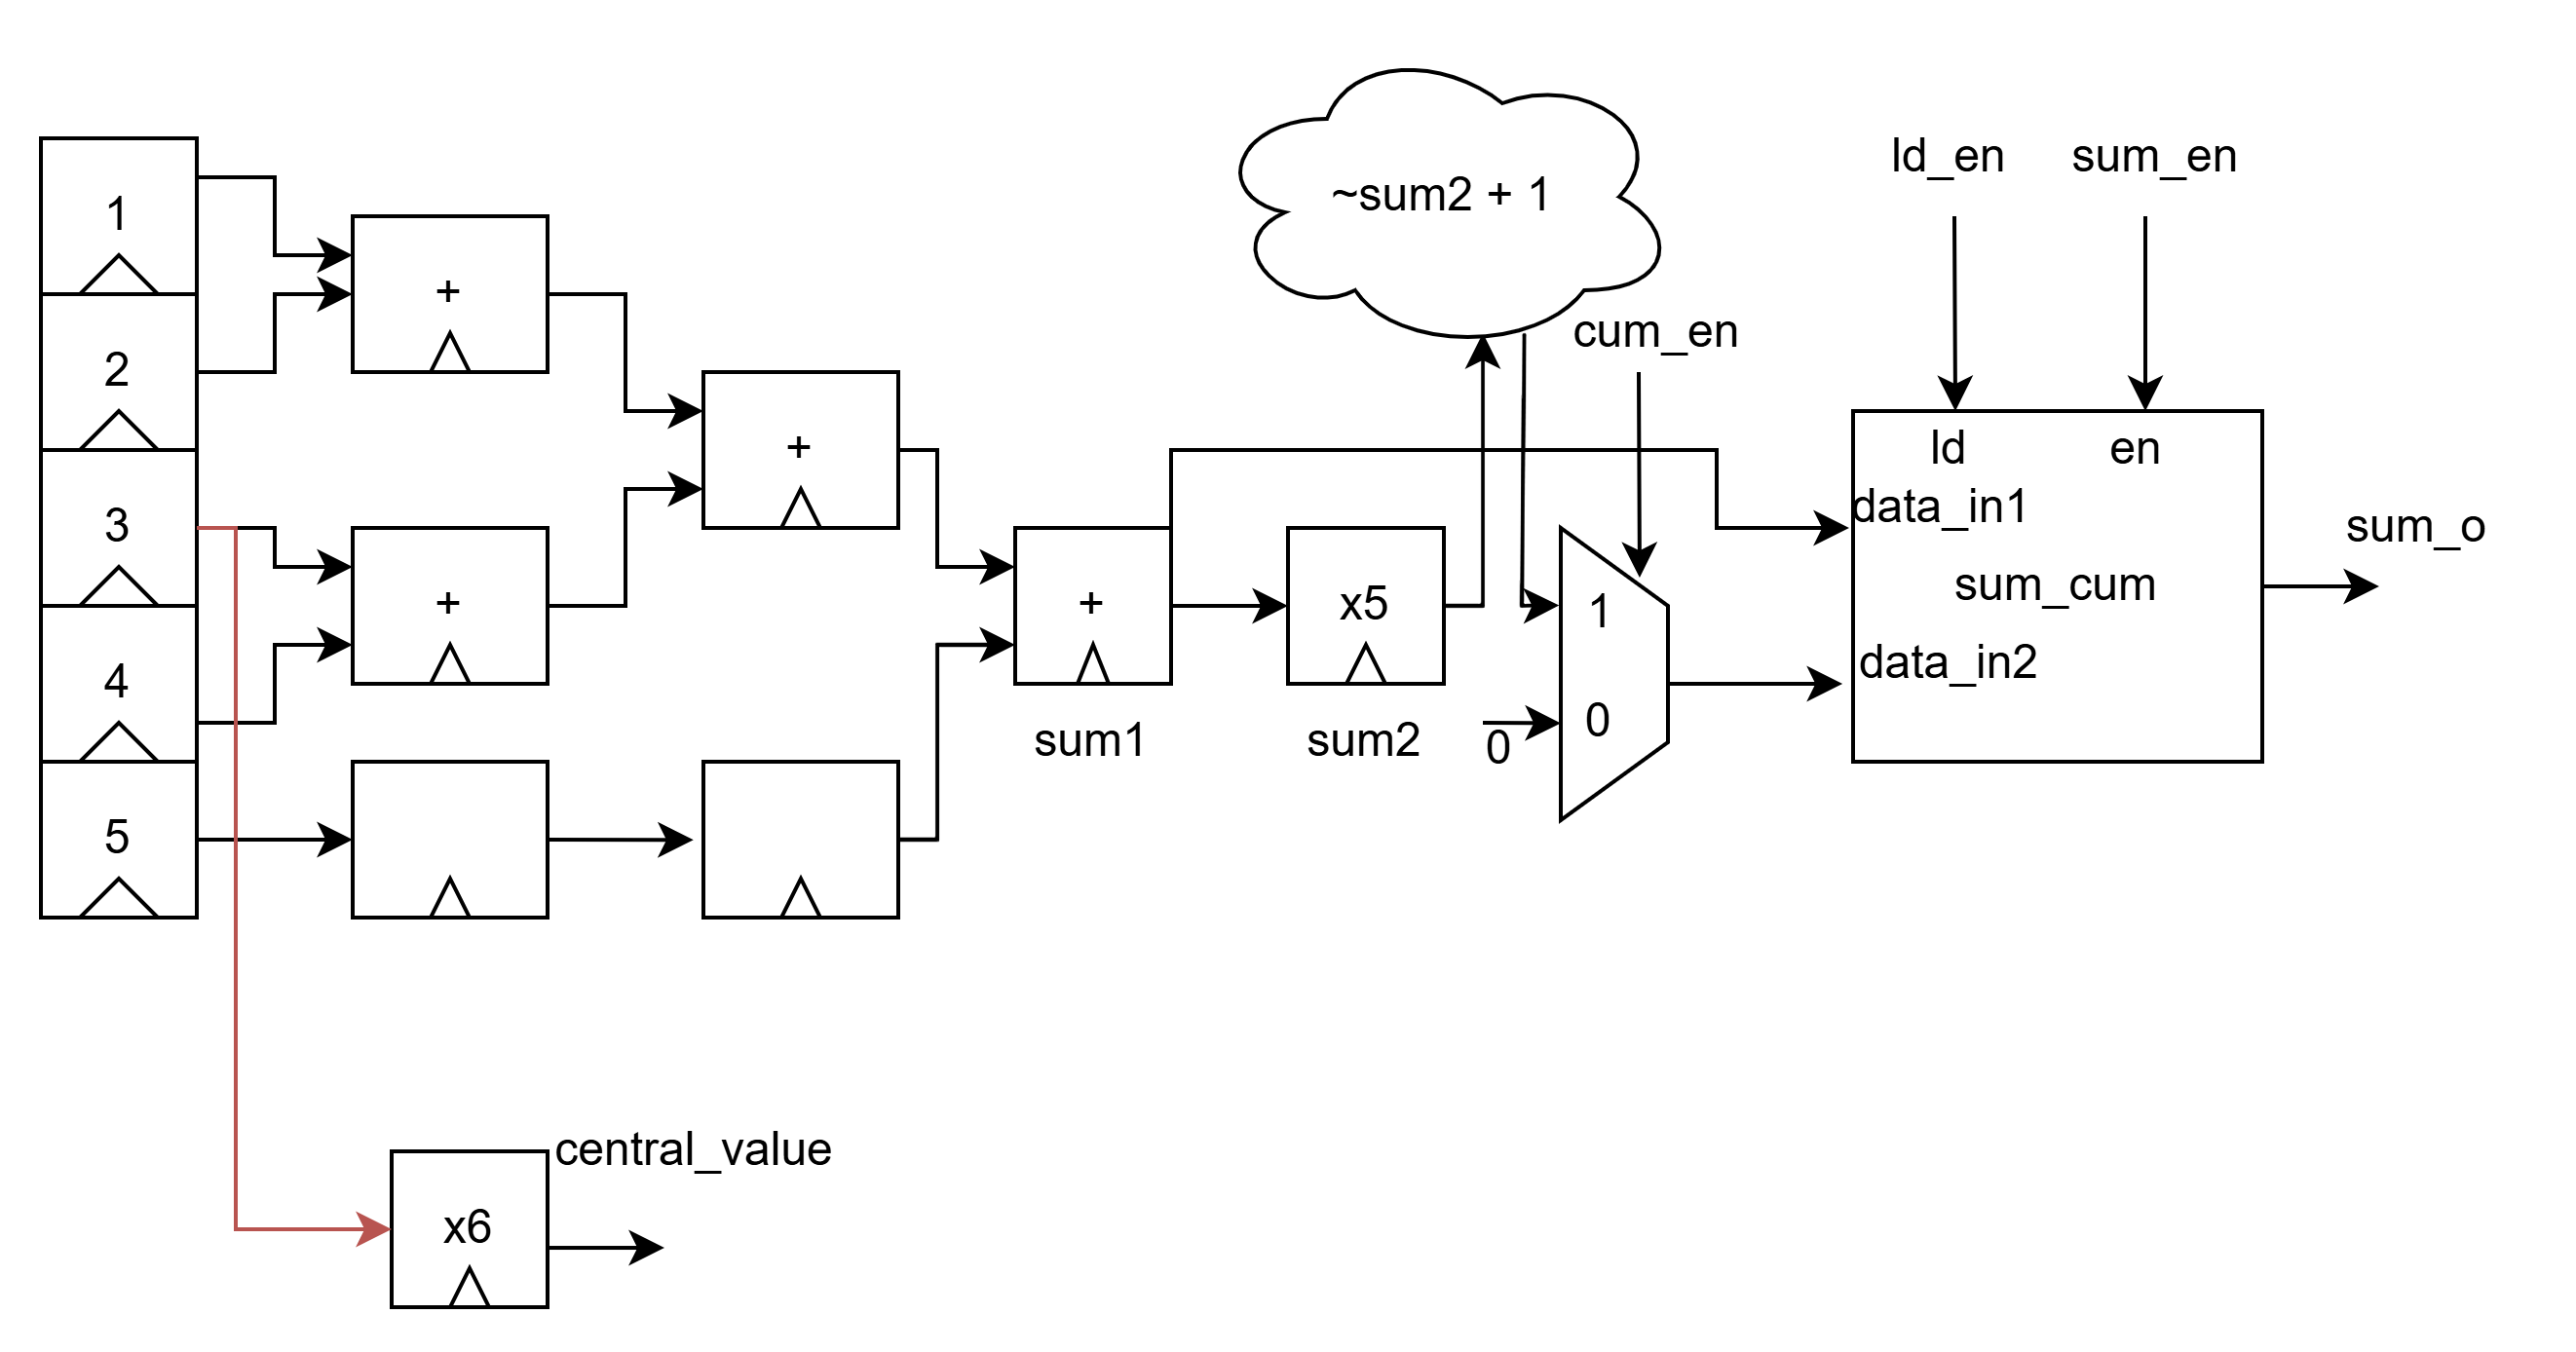
\includegraphics[width=1\linewidth]{figures/patchSumRTL_2.png}
	\caption{Kiến trúc RTL (2) của mô-đun PatchSum với r = 2}
	\label{fig:patchSumRTL_2}
\end{figure}

\section{mô-đun NIRD}
mô-đun NIRD có sơ đồ khối được mô tả theo hình \ref{fig:nirdArch} bao gồm khá nhiều mô-đun con, tuy nhiên các thành phần đó đã được mô tả một phần ở các nội dung trước, do đó trong phần này, sinh viên sẽ trình bày về kiến trúc RTL của các mô-đun con bao gồm mô-đun \textbf{Interpolation}, mô-đun \textbf{RIU2}.
\subsection{mô-đun Interpolation}
Để nội suy ra các giá trị cần thiết trong ảnh, thiết kế sẽ sử dụng phương pháp nội suy song tuyến tính. Phương pháp này sẽ tính toán giá trị một điểm dựa trên 4 điểm bên ngoài. 
\begin{figure}[!ht]
	\centering
	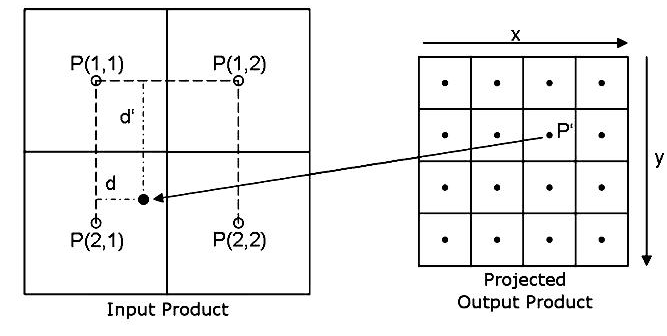
\includegraphics[width=1\linewidth]{figures/BilinearInterpolation_fig001.png.jpg}
	\caption{Nội suy song tuyến tính}
	\label{fig:BilinearInterpolationV2}
\end{figure}


Giá trị của điểm cần tính sẽ theo công thức:
\begin{equation}
	\begin{aligned}
		f(x, y) =\ &P(1,1) \cdot \frac{(x_2 - x)(y_2 - y)}{(x_2 - x_1)(y_2 - y_1)} + P(2,1) \cdot \frac{(x - x_1)(y_2 - y)}{(x_2 - x_1)(y_2 - y_1)} \\
		&+ P(1,2) \cdot \frac{(x_2 - x)(y - y_1)}{(x_2 - x_1)(y_2 - y_1)} + P(2,2) \cdot \frac{(x - x_1)(y - y_1)}{(x_2 - x_1)(y_2 - y_1)}
	\end{aligned}
\end{equation}

mô-đun Interpolation sẽ có đầu vào là 4 điểm ảnh và đầu ra là giá trị nội suy từ 4 điểm ảnh đó. Ở đây, sinh viên sử dụng một \textbf{Lookup Table} với các giá trị được tính toán trước đó từ mã python, với mỗi bán kính và góc khác nhau, sẽ có thể lấy ra được tương ứng 4 giá trị r1, r2, r3, r4 ứng với 4 giá trị nhân với 4 đầu vào. Sinh viên sử dụng số thập phân với dấu phẩy tĩnh 24 bit với 8 bit cao nhất là giá trị phần nguyên, còn lại là giá trị thập phân, như vậy giá trị nội suy lối  ra tương ứng cũng sẽ là 24 bit. 
\begin{figure}[!ht]
	\centering
	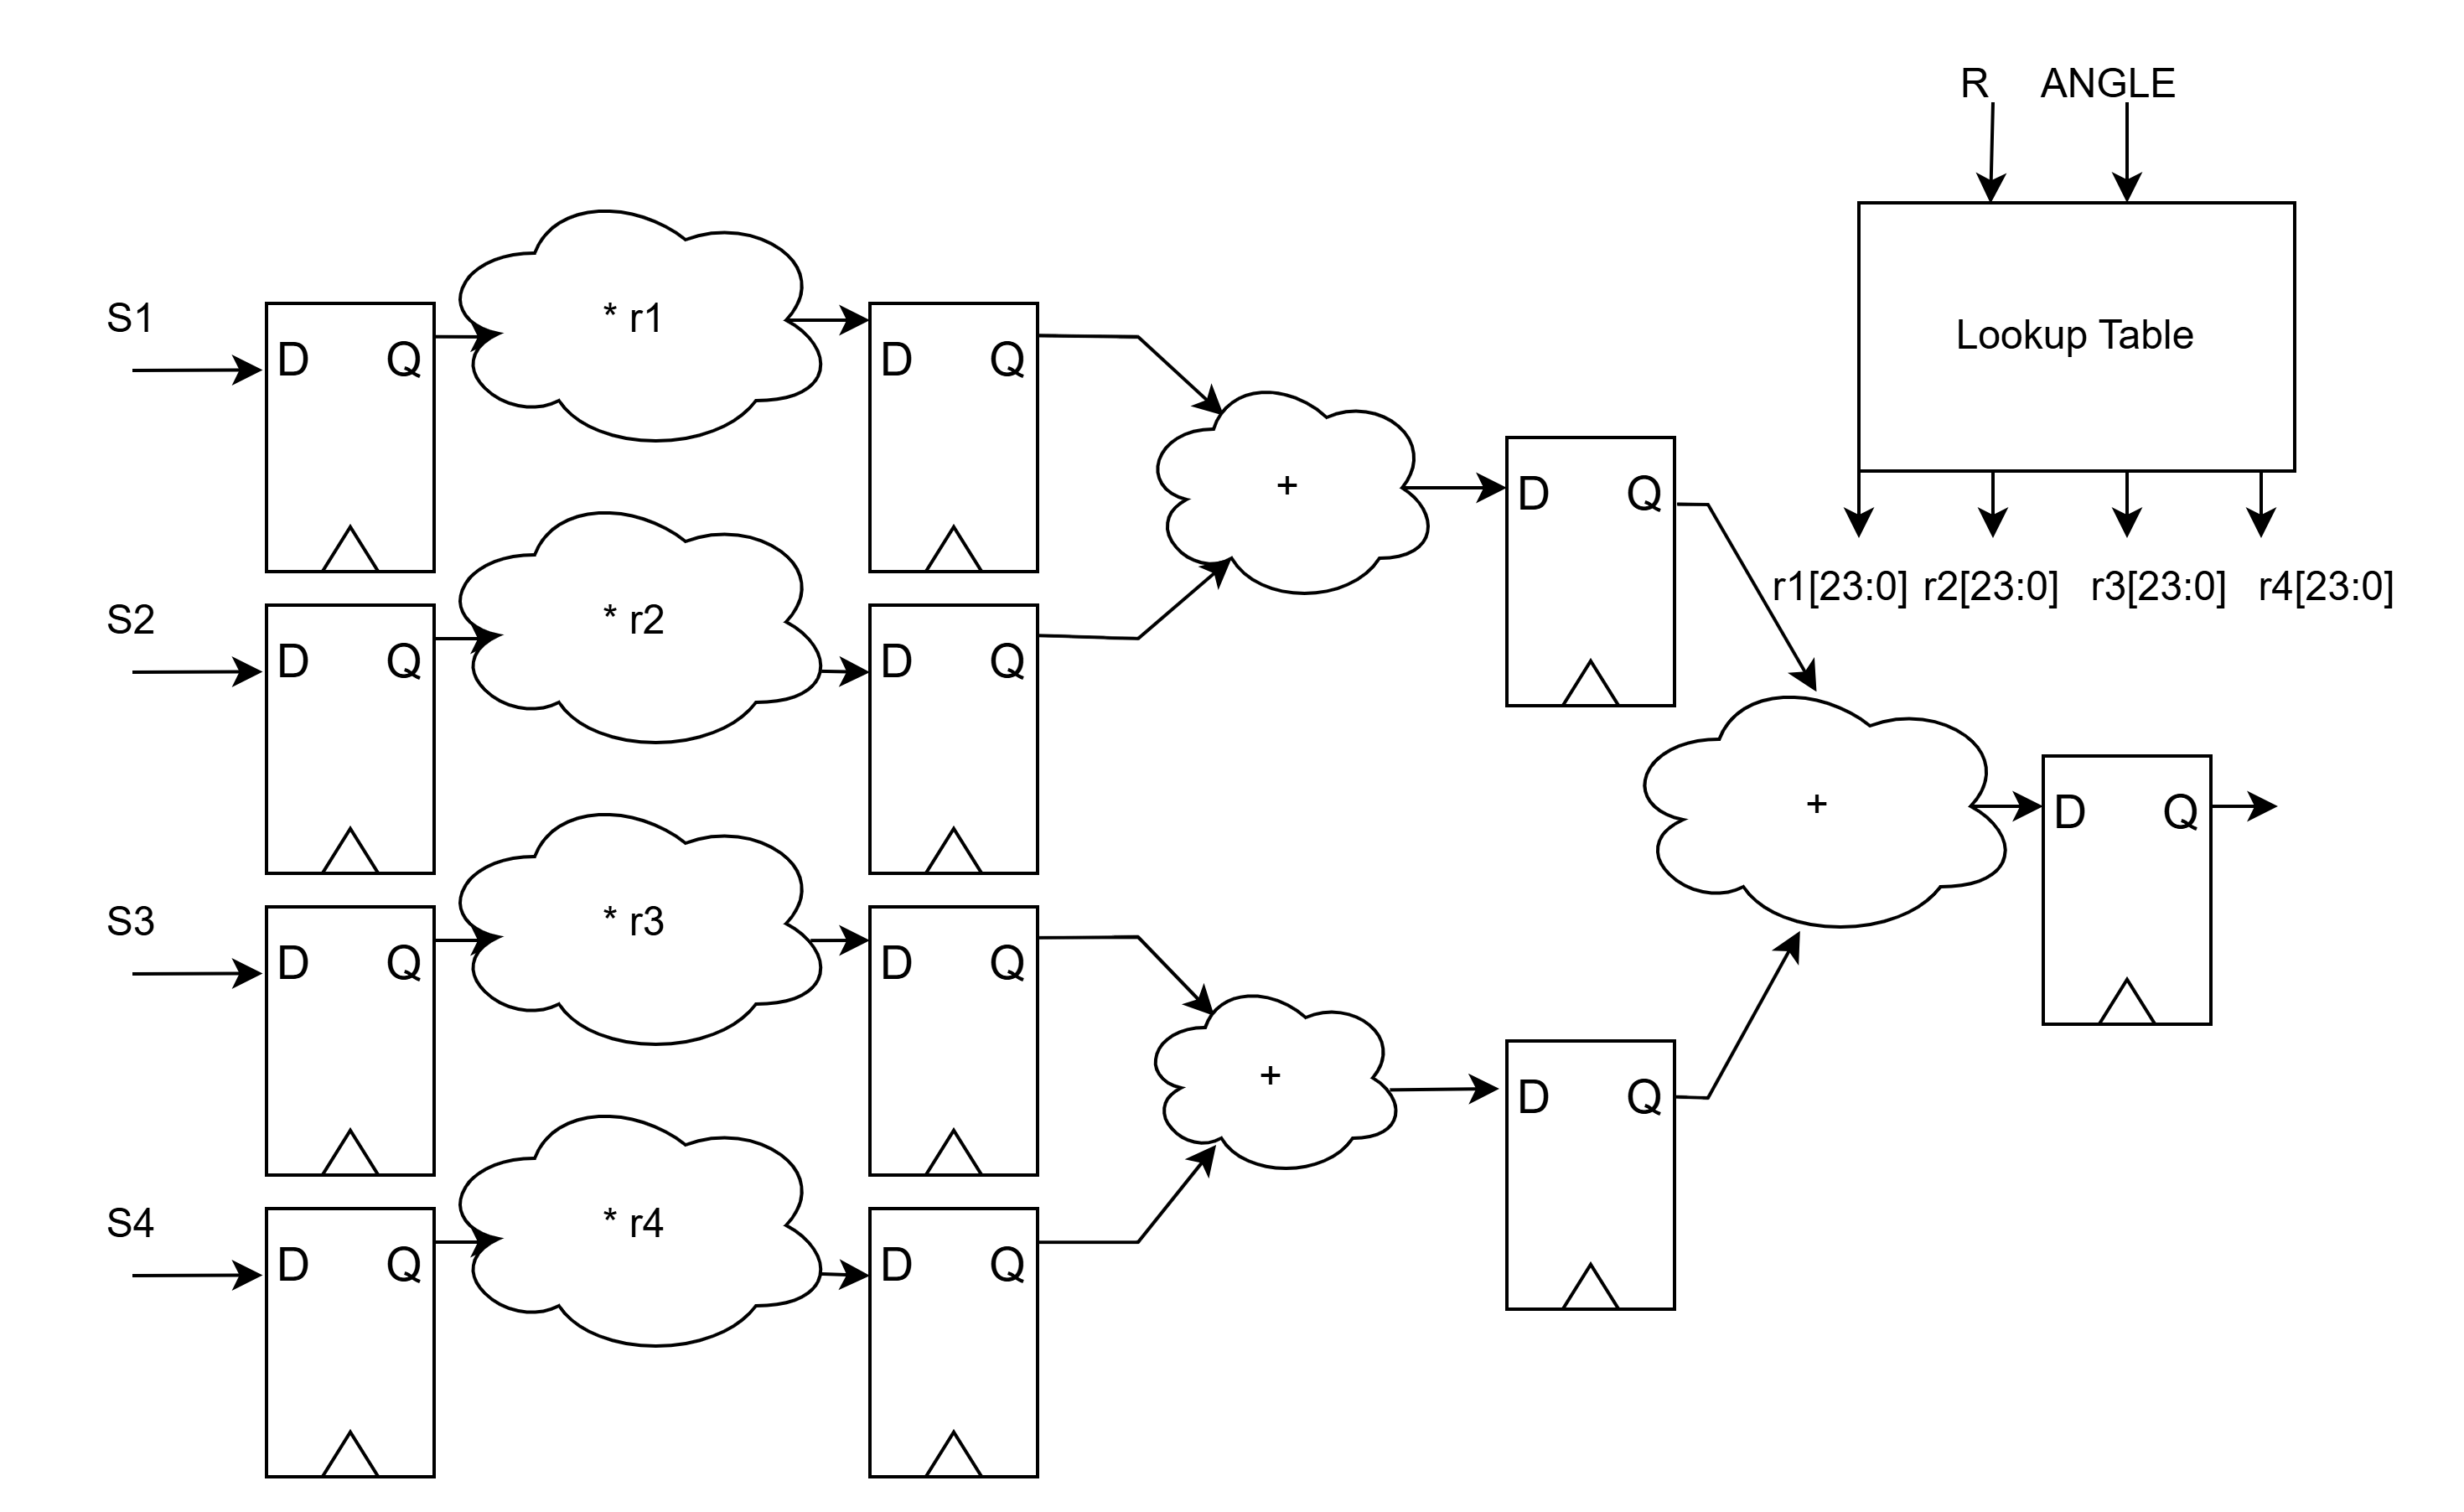
\includegraphics[width=1\linewidth]{figures/interpolationRTL.png}
	\caption{Kiến trúc RTL của mô-đun Interpolation}
	\label{fig:interpolationRTL}
\end{figure}
\subsection{mô-đun RIU2}
Mô tả với tên là RIU2 bao gồm 2 phần là RI và U2. RI là tìm giá trị nhỏ nhất khi xoay theo vòng tròn của dữ liệu trong khi đó U2 là ngưỡng của sự chuyển bit trong dữ liệu tối đa là 2. Tuy nhiên thì ta thực tế không cần quan tâm đến RI và giá trị lớn nhất hay nhỏ nhất cũng sẽ không ảnh hưởng tới số lượng chuyển bit trong dữ liệu, hay số lần chuyển bit trong dữ liệu là không đổi dù có thực hiện xoay vòng tròn. Do đó, mô-đun này sẽ tìm ra số lượng chuyển bit trong dữ liệu và quyết định đầu ra là gì. Ta biết, hai bit nếu khác nhau thì khi thực hiện phép \textbf{XOR}, giá trị đầu ra sẽ ra 1. Từ đó, ta sẽ xây dựng được kiến trúc mô tả trong hình \ref{fig:riu2RTL}.
\begin{figure}[!ht]
	\centering
	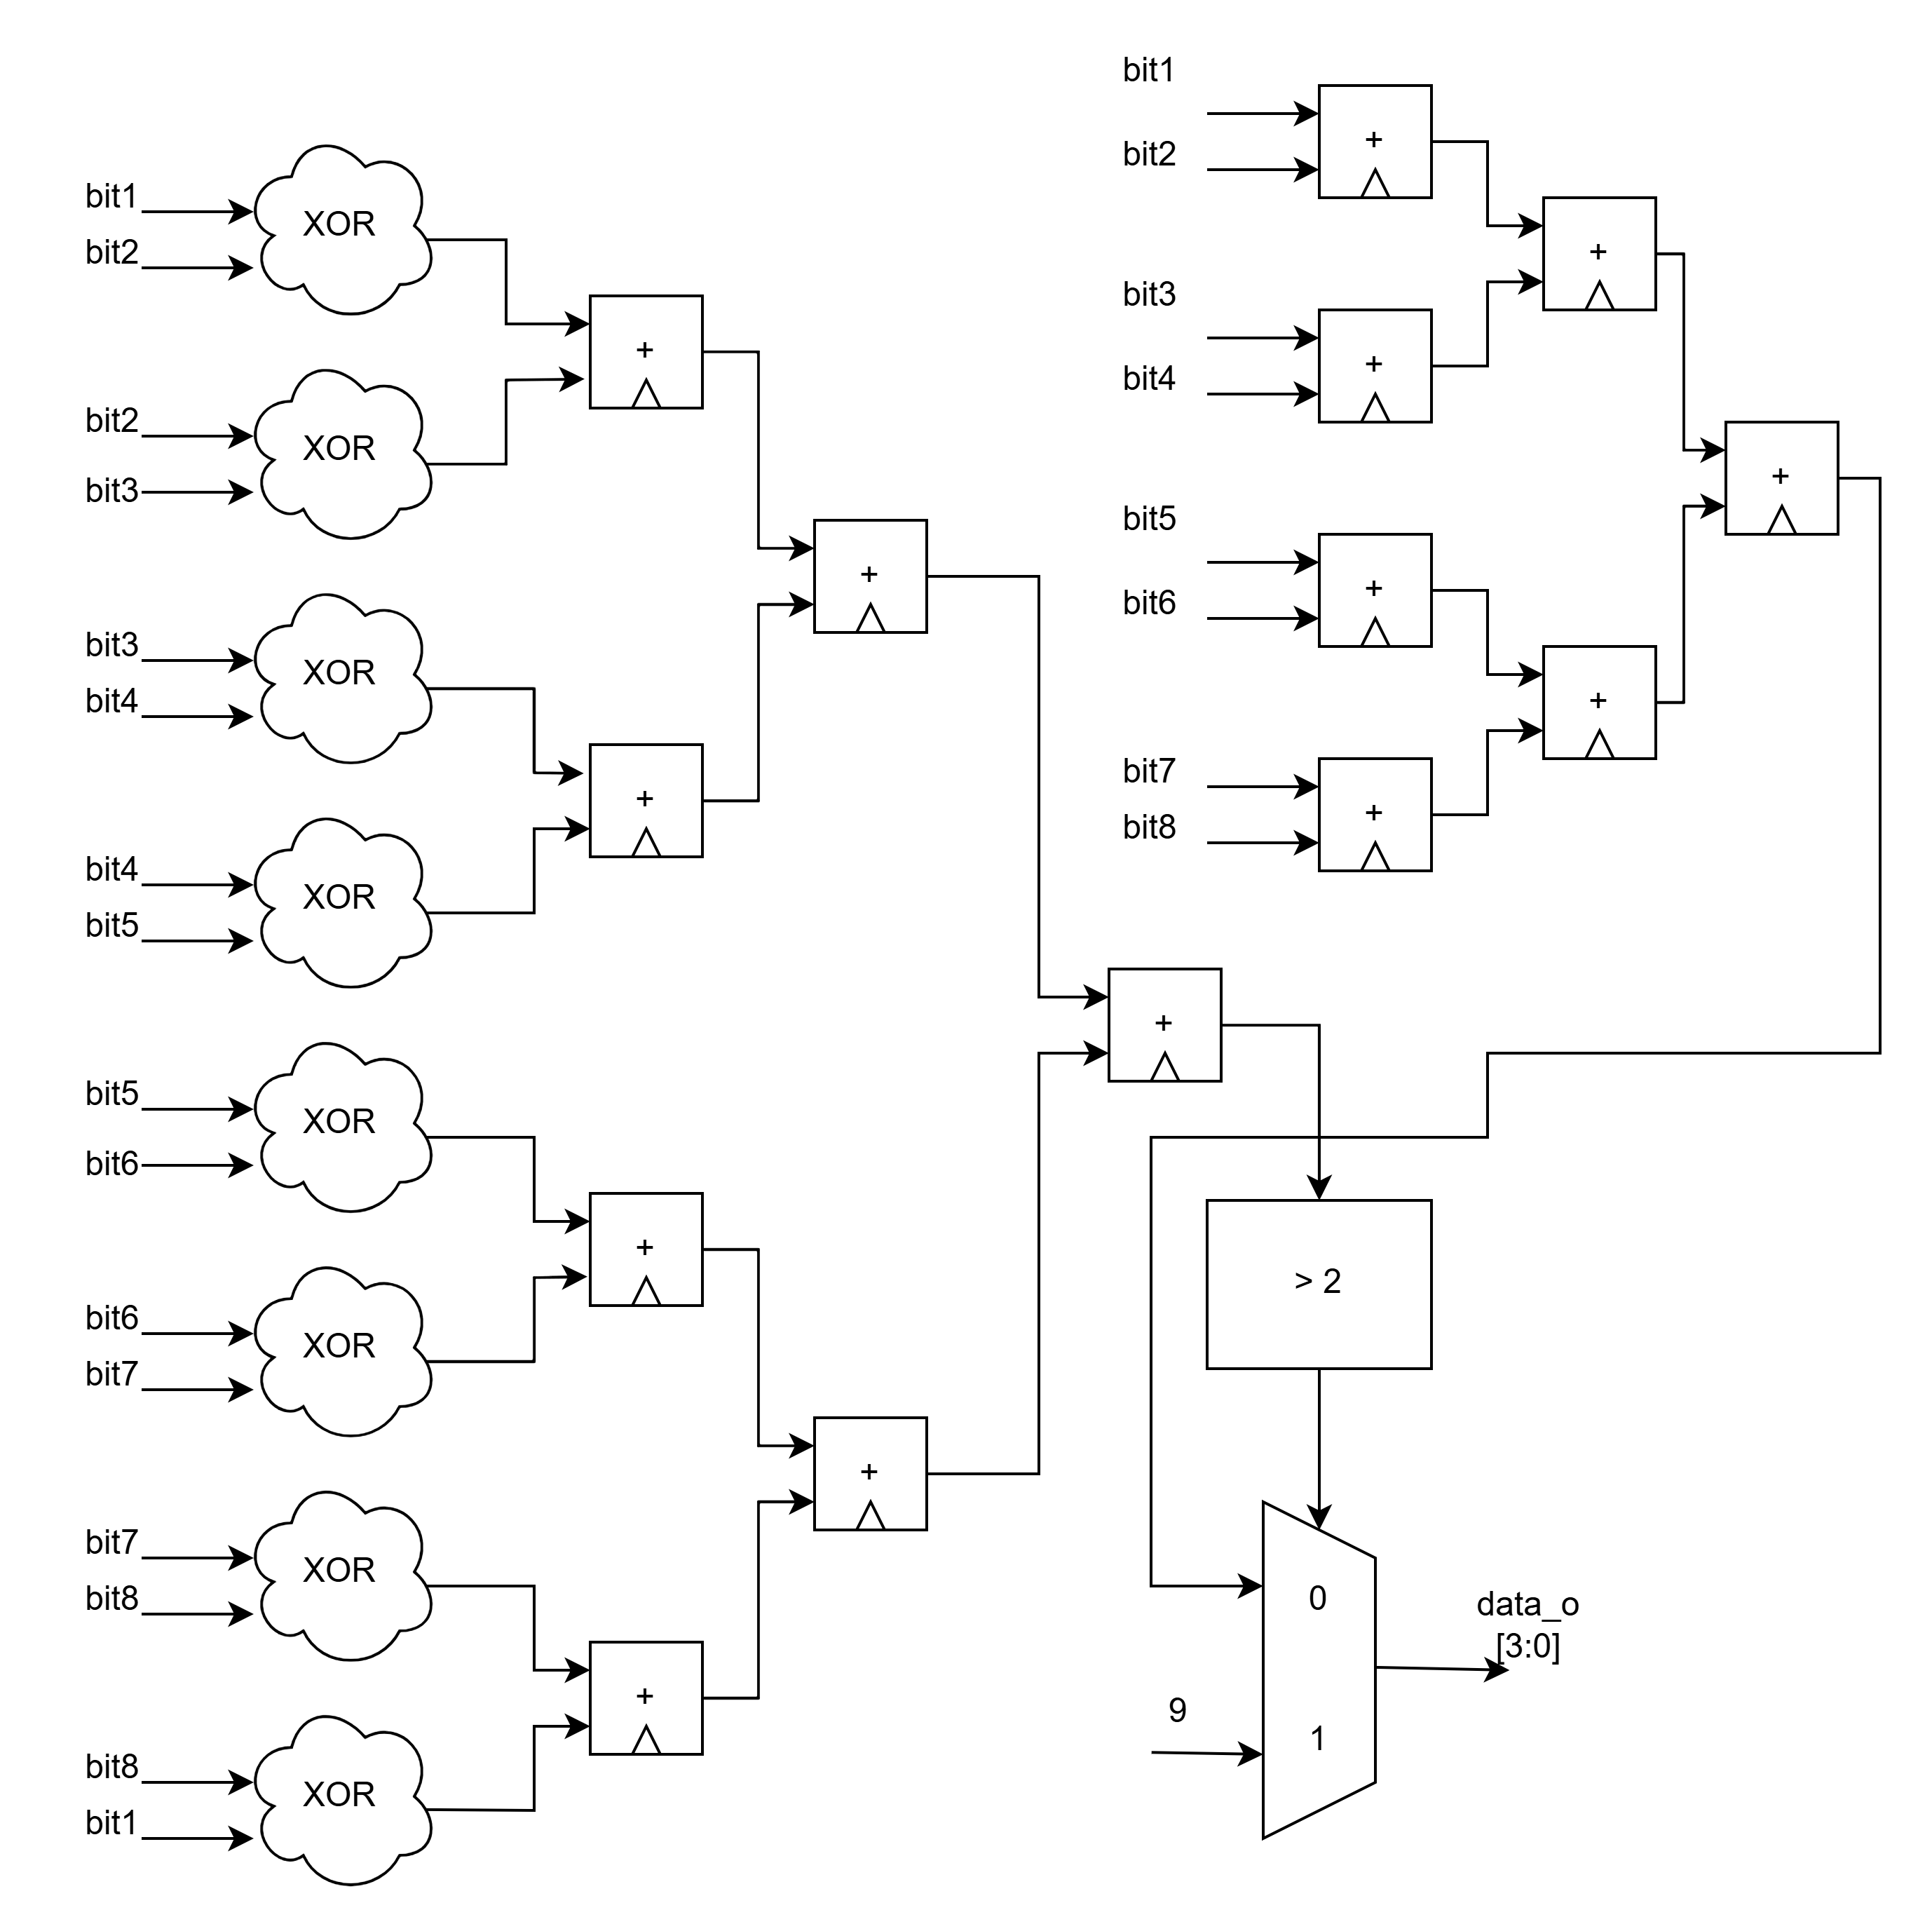
\includegraphics[width=1\linewidth]{figures/riu2RTL.png}
	\caption{Kiến trúc RTL của mô-đun RIU2}
	\label{fig:riu2RTL}
\end{figure}

\section{mô-đun JointHistogram}
mô-đun JointHistogram được triển khai theo kiến trúc và bộ điều khiển được mô tả lần lượt lại hình \ref{fig:jointHistogramRTL}, \ref{fig:jointHistogramTrans}.
\begin{figure}[!ht]
	\centering
	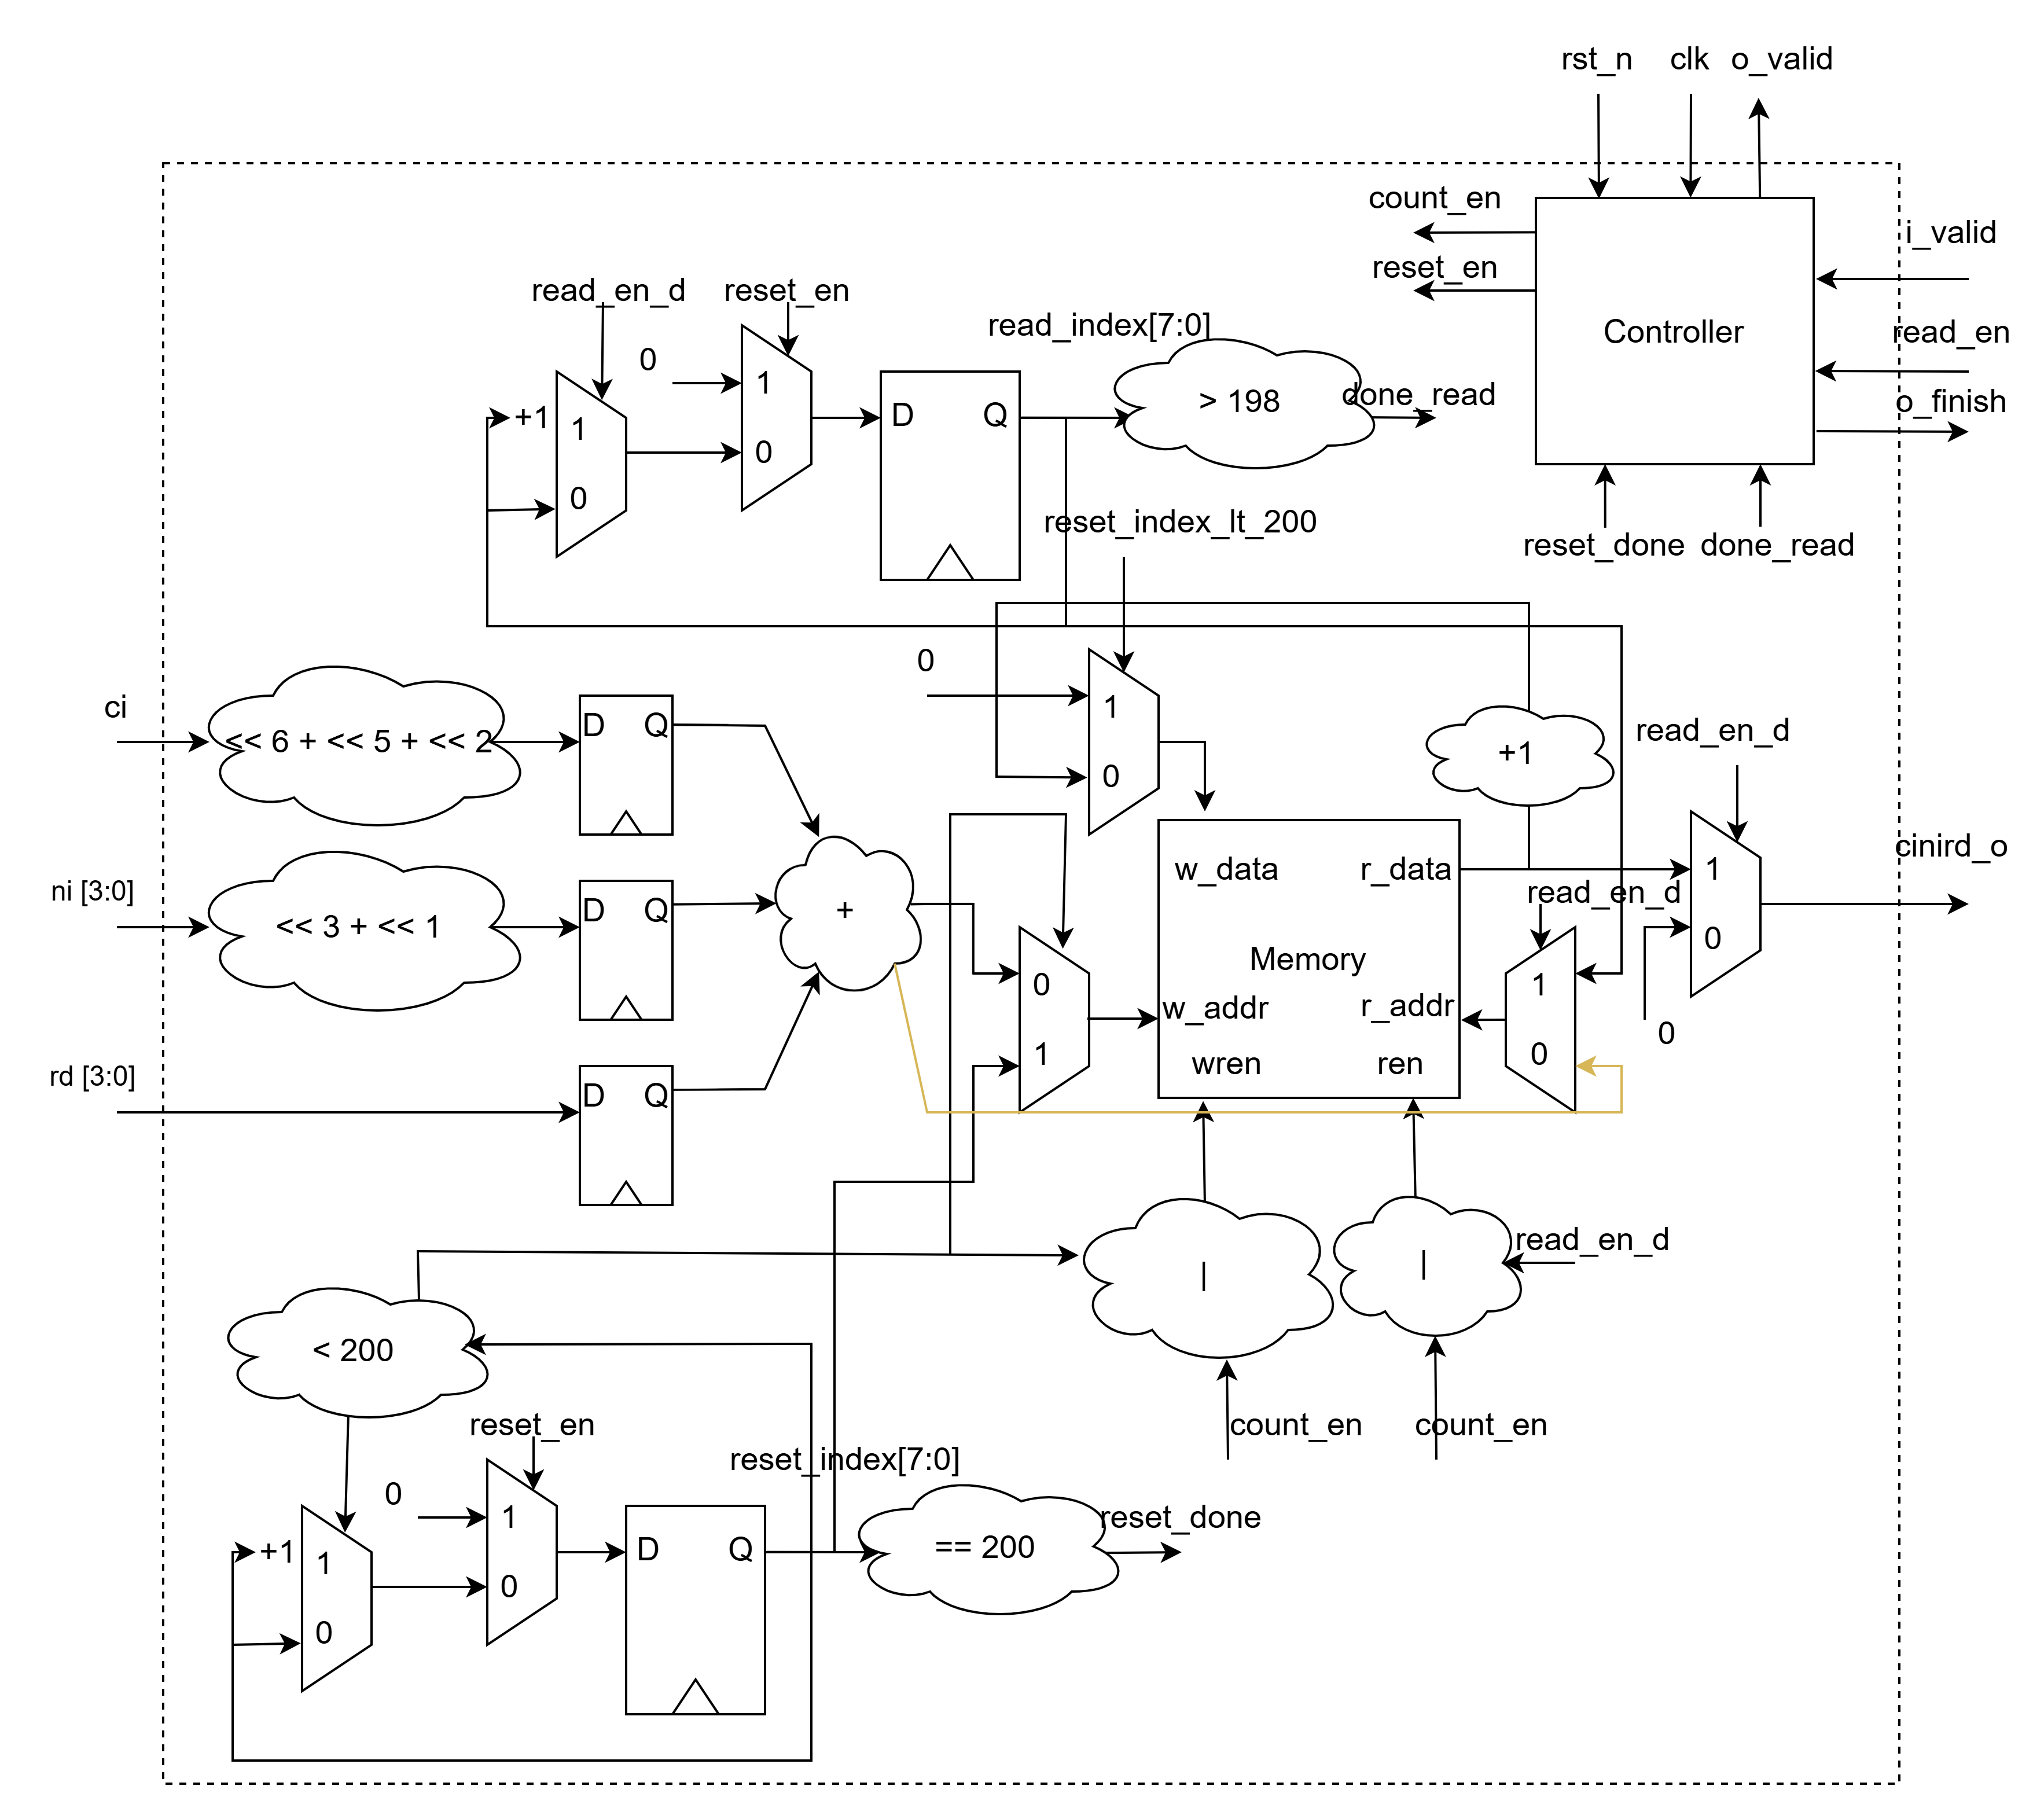
\includegraphics[width=1\linewidth]{figures/jointHistogramRTL.png}
	\caption{Kiến trúc RTL của mô-đun JointHistogram}
	\label{fig:jointHistogramRTL}
\end{figure}
\begin{figure}[!ht]
	\centering
	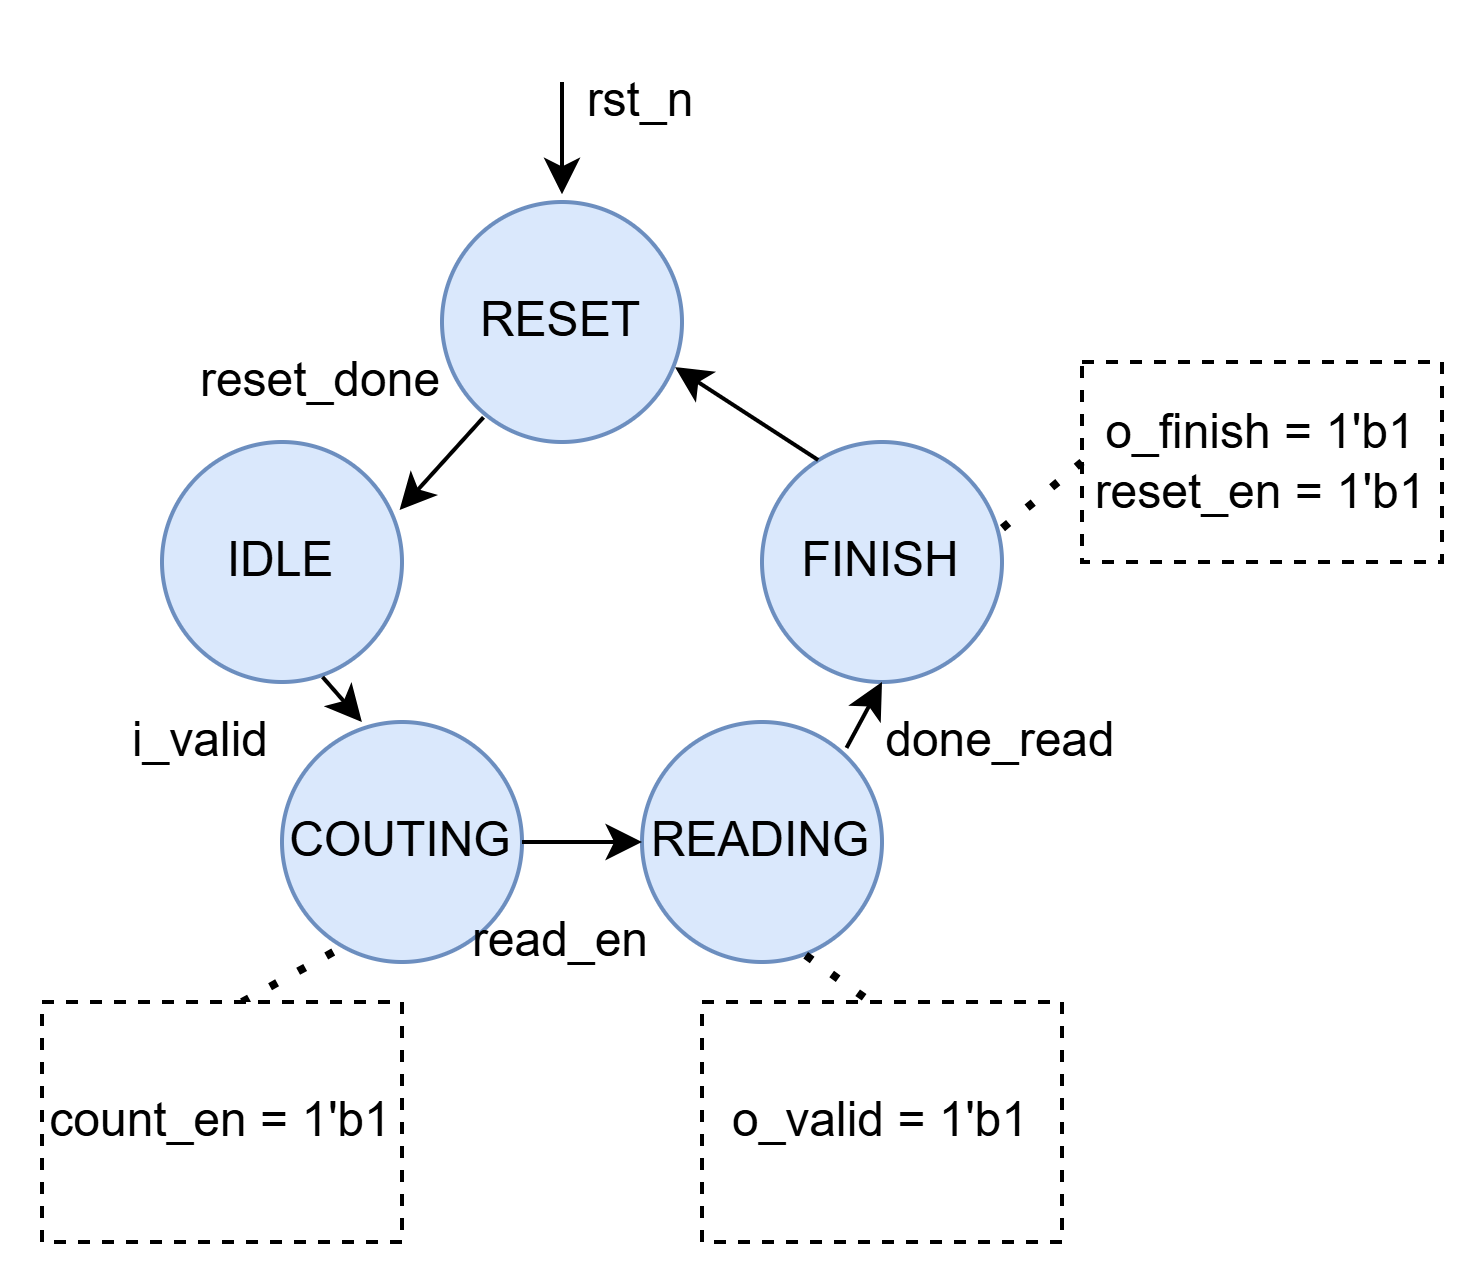
\includegraphics[width=0.5\linewidth]{figures/jointHistogramTrans.png}
	\caption{Sơ đồ chuyển trạng thái của mô-đun JointHistogram}
	\label{fig:jointHistogramTrans}
\end{figure}
\section{mô-đun MRELBP}
mô-đun MRELBP hay còn gọi là top mô-đun, là mô-đun chứa các thành phần đã nêu ở các phần trên, đồng thời còn có thêm các tín hiệu điều khiển quá trình đọc ghi. Vì mô-đun JointHistogram sẽ lưu giá trị đầu ra trong một bộ nhớ, và sẽ được đọc ra theo một yêu cầu nhất định, vì vậy, mô-đun MRELBP ngoài là một lớp chứa các thành phần trên ra còn có thêm các tín hiệu điều khiển cho mô-đun JointHistogram đọc các giá trị từ trong bộ nhớ của nó ra ngoài. Nguyên nhân là vì thực tế chỉ có 1 đầu ra mà sẽ có 3 đặc trưng ứng với 3 bán kính khác nhau, nên cần có một bộ điều phối đầu ra của cả 3 sao cho chúng là tuần tự. 

\begin{figure}[!ht]
	\centering
	\begin{minipage}[t]{0.48\linewidth}
		\centering
		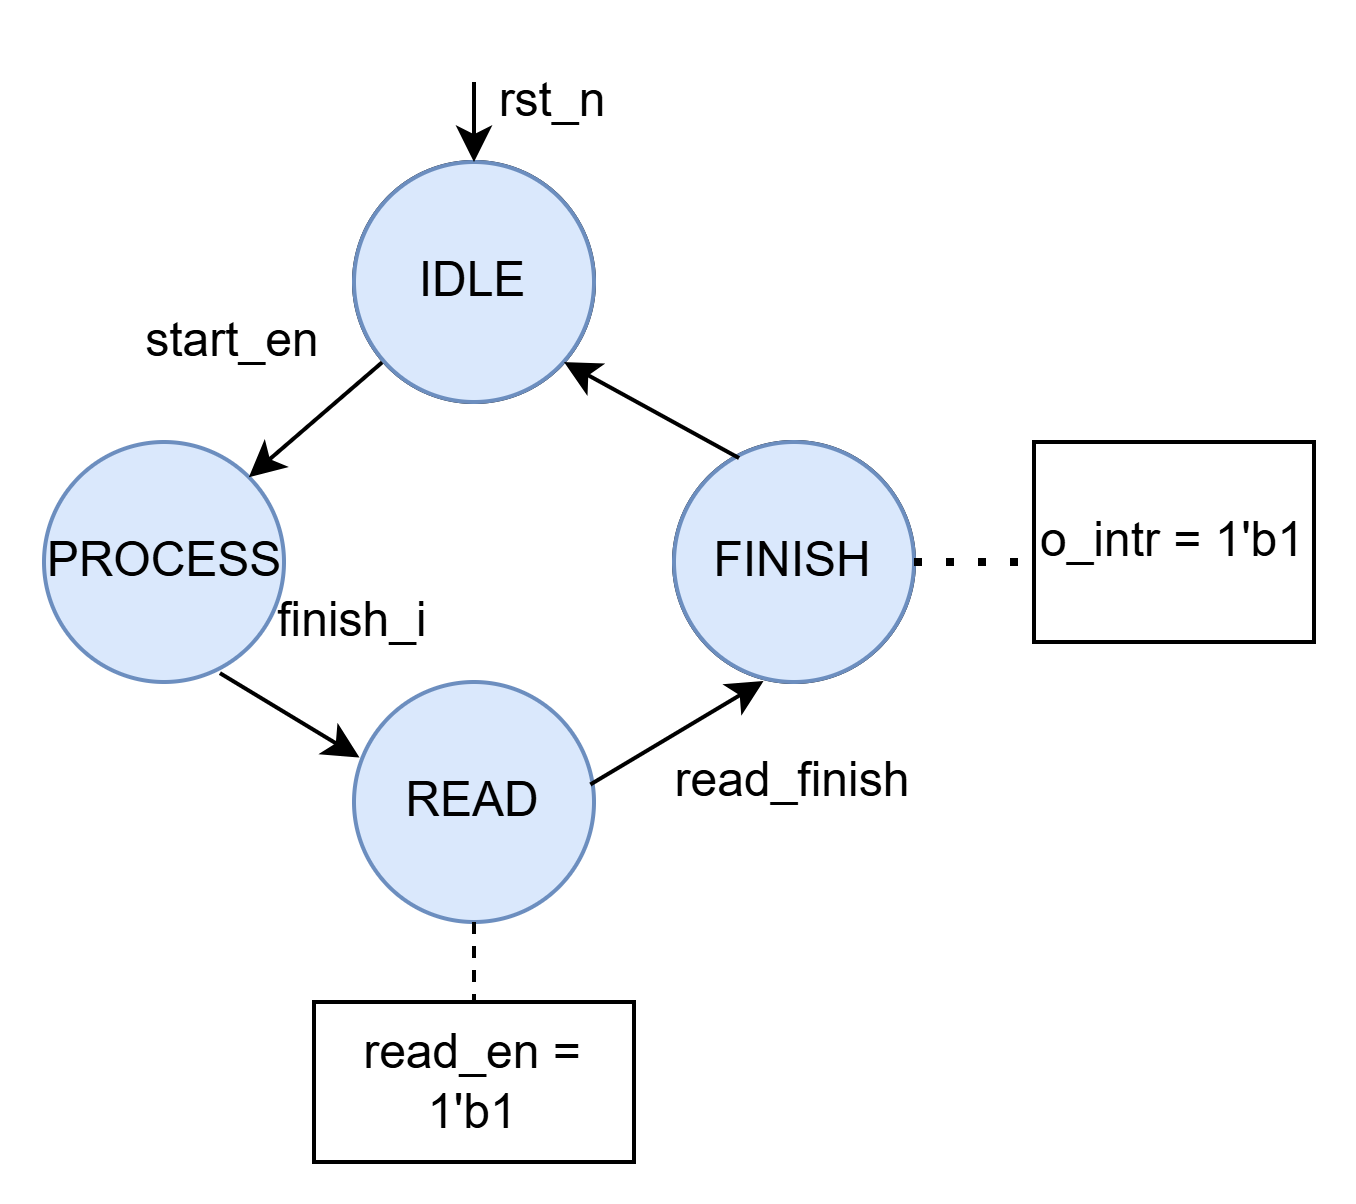
\includegraphics[width=\linewidth]{figures/topTrans.png}
		\caption{Sơ đồ chuyển trạng thái của mô-đun MRELBP}
		\label{fig:topTrans}
	\end{minipage}
	\hfill
	\begin{minipage}[t]{0.48\linewidth}
		\centering
		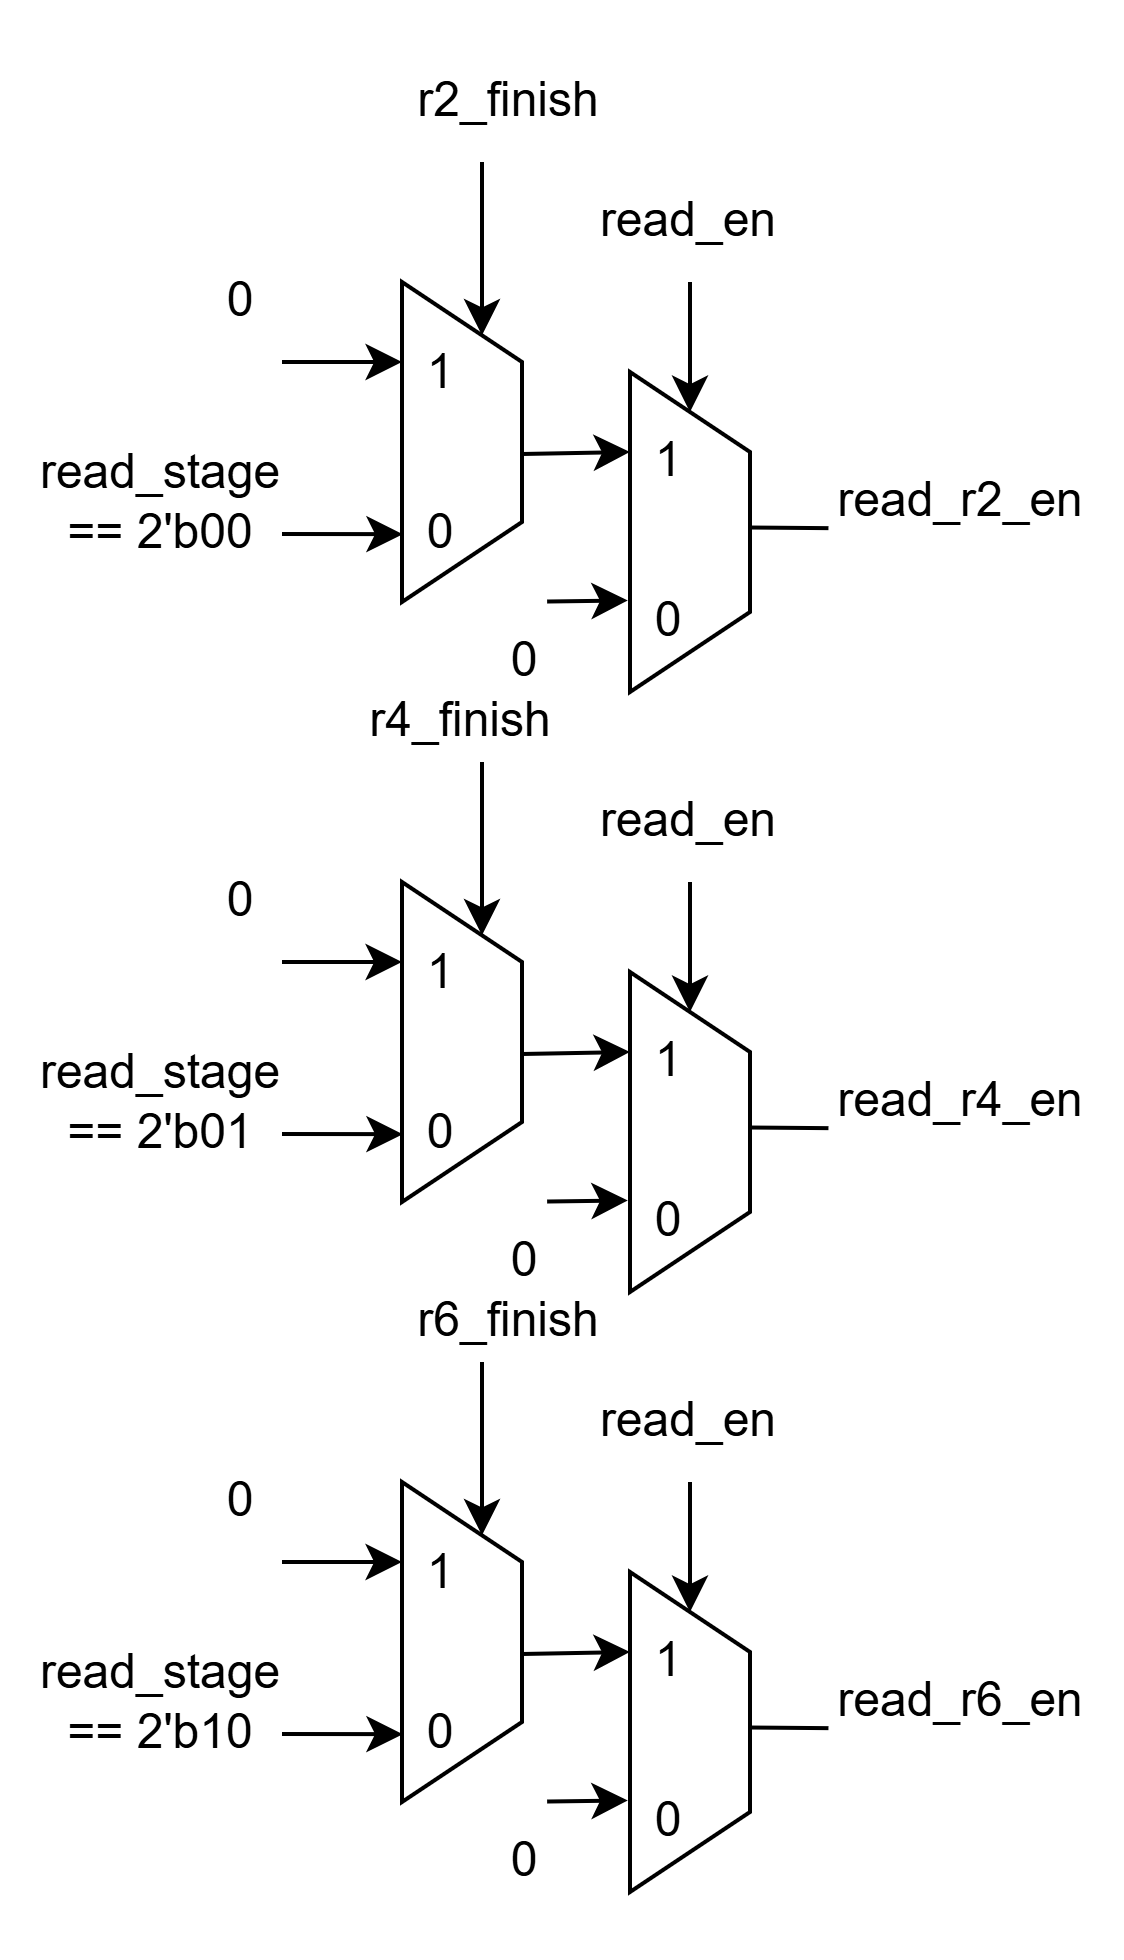
\includegraphics[width=0.8\linewidth]{figures/topRTL2.png} % Thay bằng tên hình ảnh của bạn
		\caption{Mô tả các tín hiệu yêu cầu đọc dữ liệu (1) của mô-đun MRELBP} 
		\label{fig:topRTL2}
	\end{minipage}
\end{figure}
\begin{figure}[!ht]
	\centering
	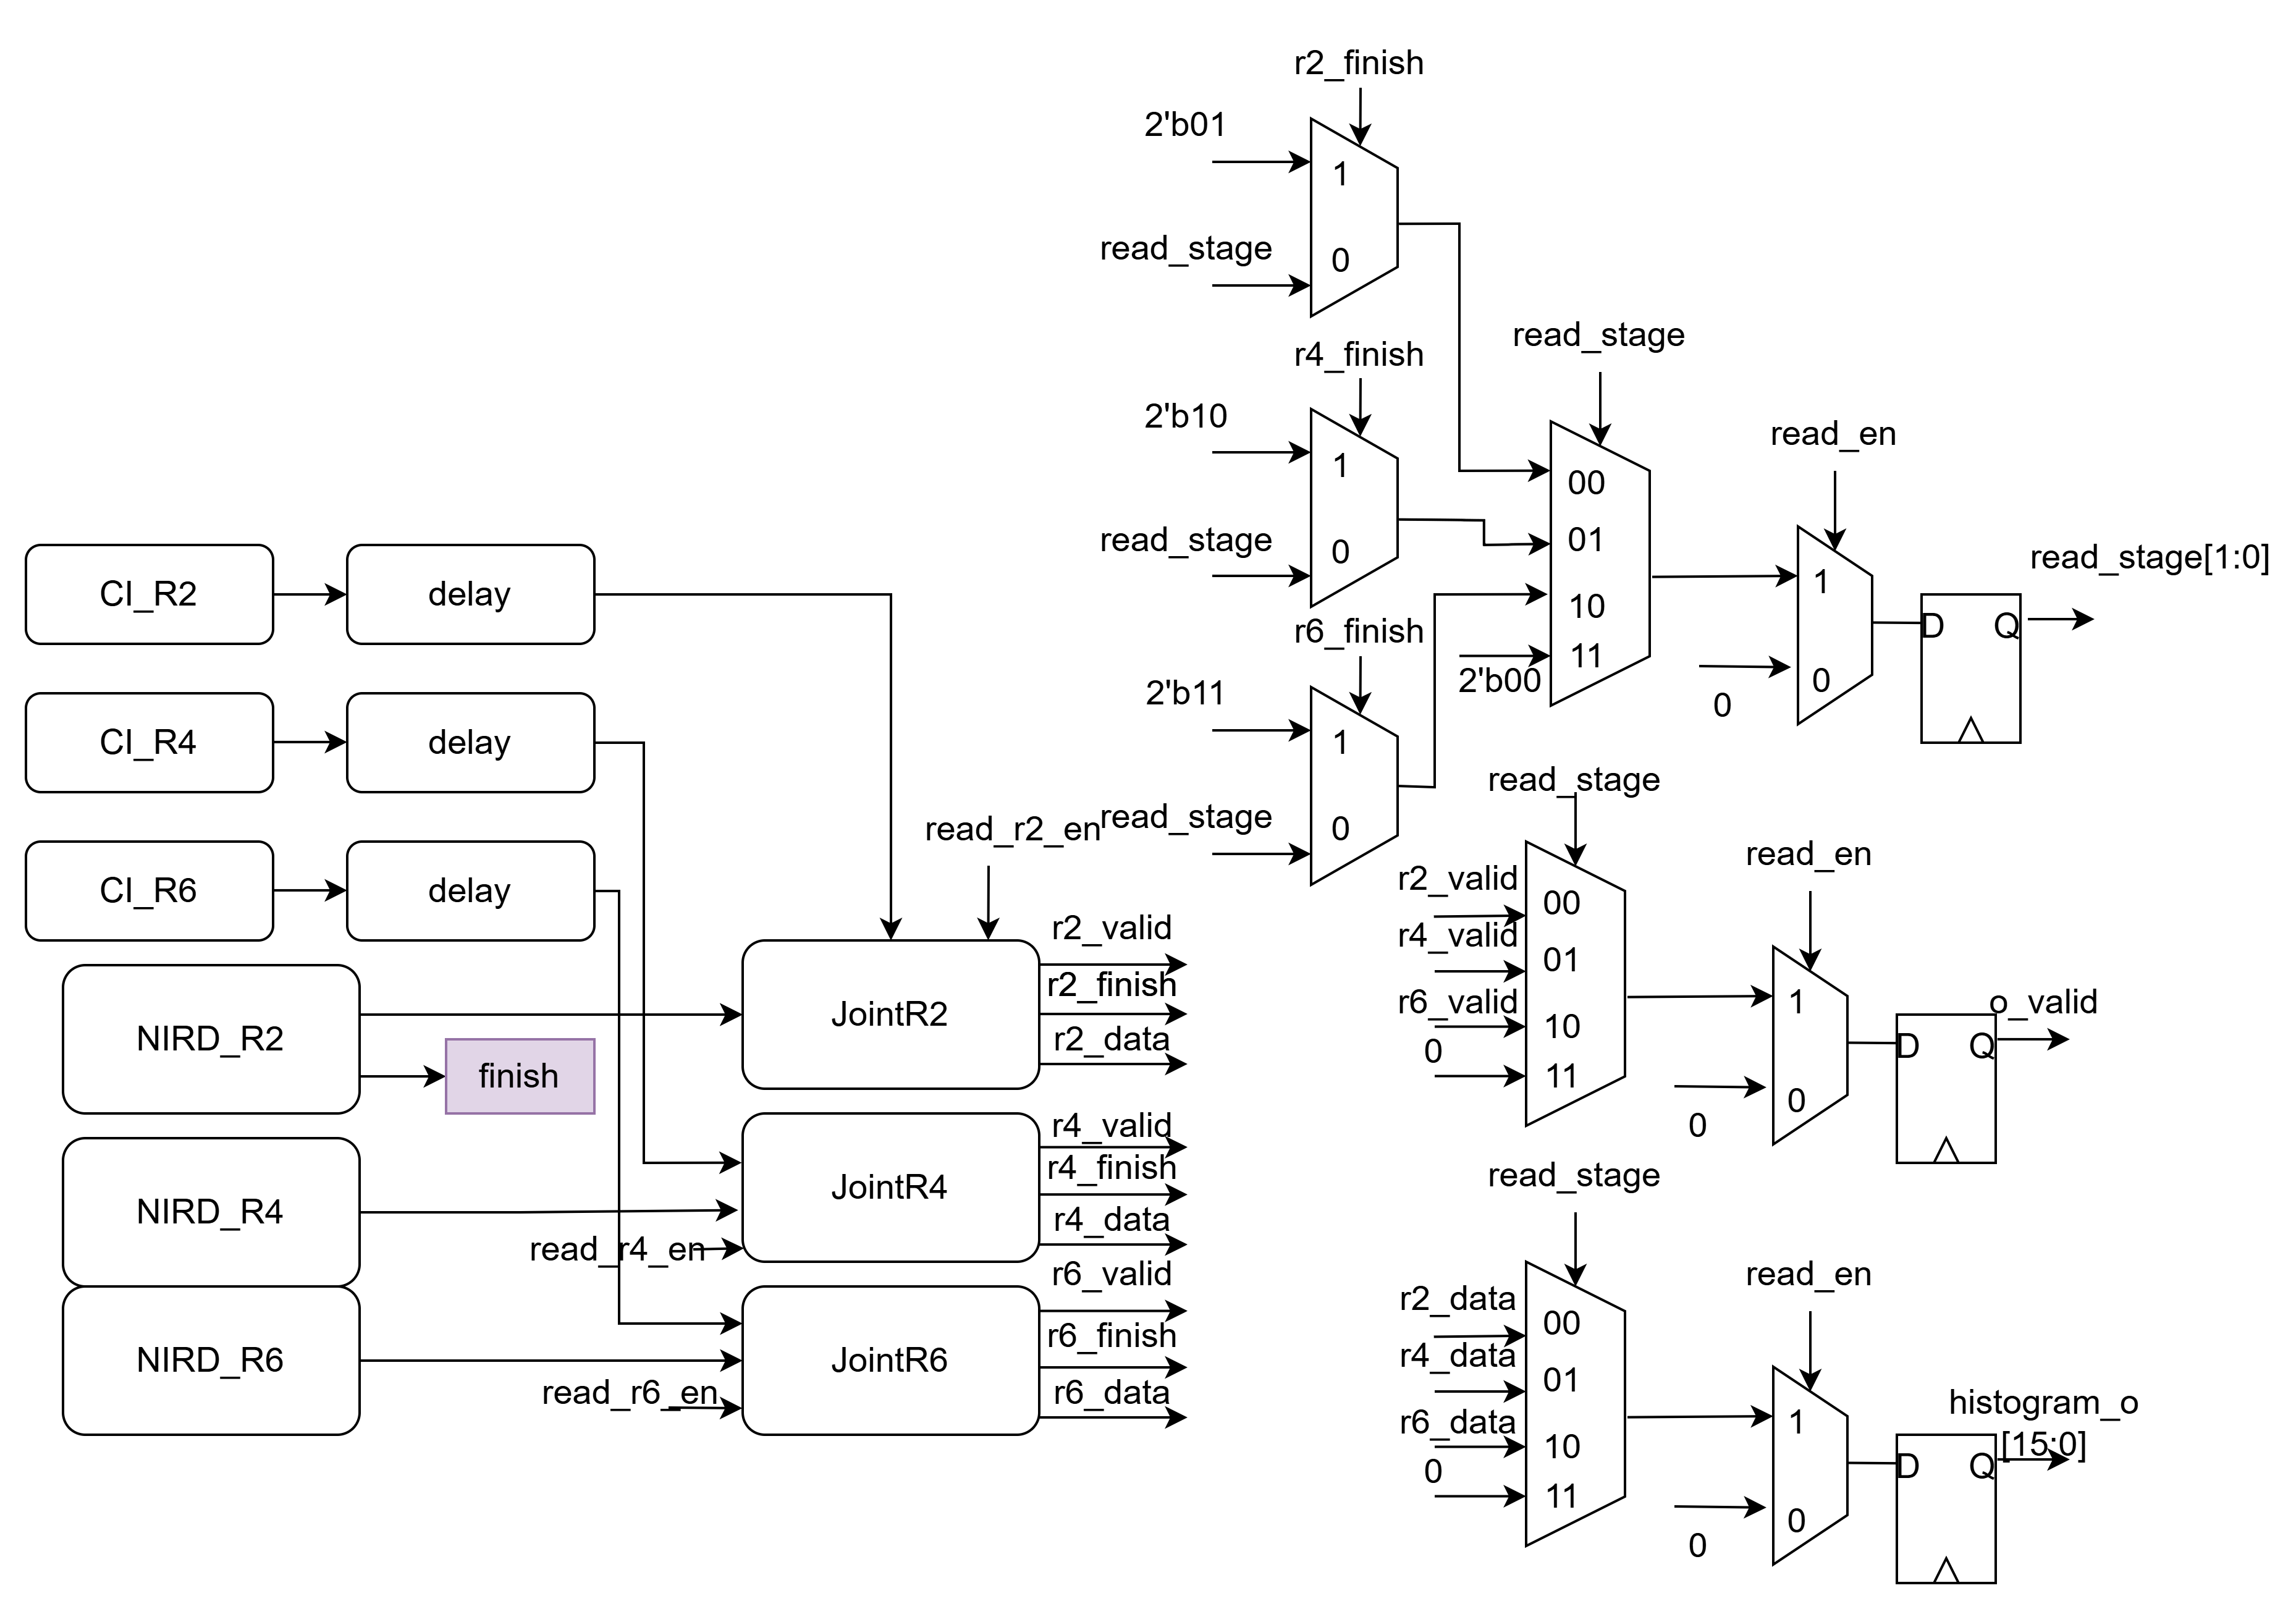
\includegraphics[width=0.9\linewidth]{figures/topRTL1.png}
	\caption{Mô tả các tín hiệu yêu cầu đọc dữ liệu (2) của mô-đun MRELBP}
	\label{fig:topRTL1}
\end{figure}
\section{Tính toán thời gian hoạt động của toàn bộ mô-đun}

\begin{table}[H]
	\centering
	\renewcommand{\arraystretch}{1.3}
		\caption{Số chu kỳ thực hiện của các mô-đun ZeroPadding}
	\begin{tabular}{|p{6cm} p{5cm} |}
		\hline
		\rowcolor{gray!30}
		\textbf{Tên mô-đun} & \textbf{Số chu kỳ thực hiện}  \\
		\hline
		Buffer6Rows  & 3 * COLS chu kỳ
		\\ \hline
		ZeroPadding3x3 & 3 chu kỳ
		\\ \hline
		ZeroPadding5x5 & 4 chu kỳ
		\\ \hline
		ZeroPadding7x7 & 5 chu kỳ
		\\ \hline
		MedianCalculation3x3 & 4 chu kỳ
		\\ \hline
		MedianCalculation5x5 & 14 chu kỳ
		\\ \hline
		MedianCalculation7x7 & 35 chu kỳ
		\\ \hline
		MedianProcessing & 3 * COLS + 40 chu kỳ

		\\ \hline
		\textbf{Tổng với kích thước ảnh H * W} & \textbf{(H + 3)* W + 635 chu kỳ}
		\\ \hline
	\end{tabular}

	\label{tab:numberOfCycleZeroPadding}
\end{table}
Minh chứng mô phỏng với các kích thước ảnh như sau:
\begin{itemize}
	\item Ảnh đầu vào kích thước 128 * 128: 17403 chu kỳ
	\item Ảnh đầu vào kích thước 256 * 256: 66939 chu kỳ
\end{itemize}

\begin{figure}[!ht]
	\centering
	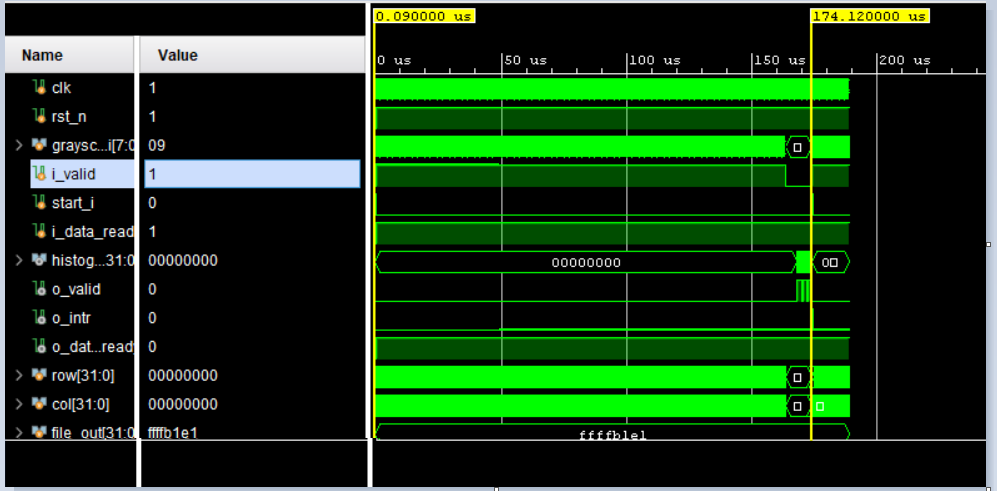
\includegraphics[width=1\linewidth]{figures/simu_time.png}
	\caption{Kết quả mô phỏng với kích thước ảnh 128x128}
	\label{fig:simu_time}
\end{figure}

